%\documentclass[10pt,a4paper]{article}
\documentclass[twoside,openright]{scrreprt}
\usepackage[utf8]{inputenc}
\usepackage{amsmath}
\usepackage{amsfonts}
\usepackage{amssymb}
\usepackage{mathtools}
\usepackage{graphicx}
\usepackage{svg}

\usepackage{stackrel}
\usepackage{caption}
\usepackage{subcaption}

\usepackage{longtable}
\usepackage{booktabs}
\usepackage{siunitx}
\usepackage{gensymb}
\usepackage{makecell}
\usepackage{bibentry}

\usepackage{layouts}
\usepackage{float}

\usepackage[msc]{tugrazthesis}


\sisetup{exponent-product=\cdot}
\sisetup{uncertainty-mode=separate}
\sisetup{range-phrase=\,--\,}
\DeclareSIUnit\od{\Delta{}mOD}
\DeclareSIUnit\radiance{\watt\per\square\meter}
\DeclareSIUnit\radExp{\joule\per\square\meter}
\sisetup{per-mode=fraction}

\begin{document}
\nobibliography*
%--- INFORMATION FOR TITLEPAGE -------------------------------------------------

% Your name including previous academic degrees (optional argument sets a different \author{}):
\thesisauthor[Firstname Lastname]{Firstname Lastname, BSc}

% Title of your thesis (optional argument sets a different \title{}):
\thesistitle[Short Thesis Title]{Title and\\Subtitle\\of the Thesis\\(up to 4 Lines)}

% Date of completion (optional argument sets a different \date{})
\thesisdate[ ]{Month Year}

% Supervisor headline (select male/female/plural version)
\supervisortitle{\germanenglish{Betreuerin/Betreuer}{Supervisor}}

% Supervisor info
\supervisor{%
  Markus Koch, academic degrees of supervisor\\
  up to 2 lines

  Institute of Experimental Physics\\
  up to 2 lines

  %optional extra information (second advisor, name of faculty, etc.)\\
  %up to 2 lines
}

% Academic degree achieved with this thesis, according to your curriculum (check curriculum and select male/female version):
\academicdegree{Diplom-Ingenieur}

\chapter{Prerequisites}

\section{Transient pump probe spectroscopy}
Using two short laser pulses a sample's response to excitation is measured. The excited states have, depending on the process of their relaxation, time scales of femtoseconds to nanoseconds. To be able to observe charge transfer between molecules and other fast relaxation pathways femtosecond time resolution pulses are needed. The response to excitation is observed as a change in optical density. Time resolution of this transient process comes from shifting the point in time where one of the pulses passes the sample relative to the other, which is usually done by a simple path length change of one of the pulses.\newline
First a probe pulse of photon flux within a wavelength range passes through the sample and the remaining intensity is detected as $\mathrm{I_{probe}(\lambda_{probe})}$. \\
Secondly, after a period of time to allow the sample to relax back to its initial state, a pump pulse $\mathrm{I_{pump}(\lambda_{pump})}$ excites a volume of the sample. This leads to a direct change of the optical density of the excited sample volume, which alters the transmission of the probe photons $\mathrm{I_{pump-probe}(\lambda_{probe}, \lambda_{pump}, \Delta t)}$ depending on the time delay $\Delta t$ between the pulses passing the sample volume and the pump and probe wavelengths $\lambda_{pump}/\lambda_{probe}$ respectively. \\
The change in absorptive properties of the sample depending on the pump pulse is characterised in the transient absorbance $\mathrm{\Delta A}$, which often is given in orders of magnitude of the optical density. It is defined as seen in eq. \ref{eq:TA}.
\begin{equation}\label{eq:TA}
\begin{split}
\Delta A(\lambda_{\mathrm{pump}}, \lambda_{\mathrm{probe}}, \Delta t)&=-\log _{10}\left(\frac{I_{\mathrm{pump}-\mathrm{probe}}\left(\lambda_{\mathrm{pump}}, \lambda_{\mathrm{probe}}, \Delta t\right)}{I_{\mathrm{probe}}\left(\lambda_{\mathrm{probe}}\right)}\right)\\
&=-\log _{10}\left(1+\frac{\Delta I_{\mathrm{probe}}\left(\lambda_{\mathrm{pump}}, \lambda_{\mathrm{probe}}, \Delta t\right)}{I_{\mathrm{probe}}\left(\lambda_{\mathrm{probe}}\right)}\right)
\end{split}
\end{equation}

\section{Transient effects in pump probe spectroscopy}
There are several types of contrast within pump probe spectroscopy. Processes like two-photon-fluorescence, second or third harmonic generation (and SRS?) are too high power for our samples and would lead to immediate deactivation. They are thus not going to be addressed further with respect to the sample transient processes. The most relevant ones for this experimental setup are:\cite{10.1063/1.5129123}
\begin{itemize}
\item Stimulated Emission (SE): Possible in cases where a state below or at the  excited level has a transition to a lower state corresponding to the other photon wavelength used. This could be either pump or probe exciting and then the other leading to stimulated emission. However as the change in the probe is measured only contrast for pump excitation with probe stimulated emission is possible. The emitted photons are of identical energy to the probe pulse and thus an increase in transmission is observed.
\item Ground State Depletion (GSD): By moving part of the ground state population to different energy levels the probe pulse sees a smaller absorption cross-section. This is seen as a positive change in transmission. The signal returns by an exponential, sometimes multi-exponential when multiple states are excited, decay to the starting transmission value as the molecules relax back to the ground state.
\item Excited State Absorption (ESA): Similar to GSD a population transfer from the ground state happens, however with this population transfer now a state previously not accessible with the probe pulse becomes accessible, thus leading to an increase in absorption and a reduction of transmission.
\item Photothermal Effect: Due to heating from strong absorption of the pump beam a change in the refractive index changes the propagation path of the probe beam. It can be avoided by having a larger numerical aperture in the rear focusing element, the condensor, than for the front focusing element and changing modulation frequency.
\item Cross Phase Modulation (XPM): Through the optical Kerr effect the refractive index changes when both pump and probe beam are temporally overlapped within the sample. This may be used to check the instrumental response of the transient absorption microscope. It can be avoided like the photothermal effect by a larger condensor numerical aperture.
\item Stimulated Raman Scattering: In case the energy difference between pump and probe corresponds to a raman active state a photon transfer from the higher energy beam to the lower energy beam may happen. For this there needs to be temporal overlap of the beams.
\end{itemize}

These processes may manifest at the same time, thus concealing other processes with the opposite influence on the transient opacity. This is not so much of concern for processes like XPM or stimulated raman scattering, because they require temporal overlap of pump and probe pulse and thus only influence a short range within the time delay based on the pulse lengths. ESA and GSD are measured within a regime linear to the pump irradiance of the sample, where the peak power of the pulse is not high enough for nonlinear optical processes. For this reason the temporal pulse shape is not so important for the classification of these measurements, other than time resolution. Thus it makes sense to write powers used here for pump and probe as dose per area per shot ($\mathrm{\frac{J}{m^2}}$), to also avoid confusing values due to different repetition rates of pump and probe pulses.\\

To record a GSD spectrum simply an excitation from GS has to be available for the probe beam spectrum. For ESA state energies probed are a combination of an excited state reachable by the pump and then the probe beam spectrum. The available photon wavelengths for pump and probe may be seen in tab. \ref{tab:NOPAs}. An important factor is that neither pump or probe are mono-energetic light and they will excite off center wavelengths.

\begin{figure}[hbtp]
\centering
\begin{subfigure}[t]{0.3\textwidth}
\centering
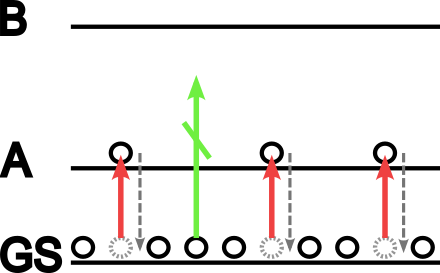
\includegraphics[width=\linewidth]{images/TA-explanationProbeOnly.png}
\caption{Probing of sample in groundstate at $t-t_{sample\, pump} < 0$ at two different photon energies.\label{fig:probeOnly}}
\end{subfigure}
\hfill
\begin{subfigure}[t]{0.3\textwidth}
\centering
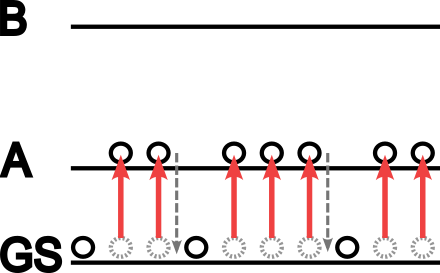
\includegraphics[width=\linewidth]{images/TA-explanationPumpOnly.png}
\caption{Pumping of sample in groundstate}
\end{subfigure}
\hfill
\begin{subfigure}[t]{0.3\textwidth}
\centering
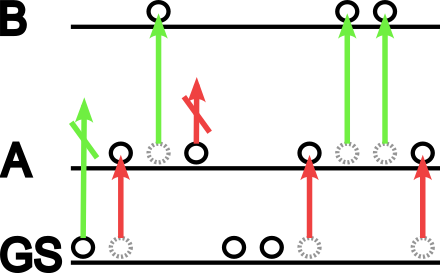
\includegraphics[width=\linewidth]{images/TA-explanation-probe-after-pump.png}
\caption{Probing of sample  after pump at $t-t_{sample\, pump} > 0$ at two different photon energies. Green experiences ESA and red experiences GSD.\label{fig:probeAfterPump}}
\end{subfigure}
\caption{Principle of pump probe spectroscopy with ESA and GSD. GS is the groundstate of the sample without excitation. A is a low energy state that may be excited from GS. B is a higher energy excited state that may be populated from both GS and A, however selection rules may apply. Fig. \ref{fig:probeOnly} shows the probe passing the sample at a time where no excitation has happened yet. This is the case both for the reference probe only measurement as well as for the pump-probe measurement ahead of temporal overlap.\label{fig:CompendiumTA}}
\end{figure}


\textbf{
Tell them about what happens if probe intensity is too high. -> self GSD of probe that leads to bad measurement values; maybe do in reliability}
\textbf{insert image from source}
\subsubsection{Delay scan in detail}
\textbf{show example of delay scan}
A single measurement point usually consists of multiple delay scans averaged together. The relative absorbance signal of a delay scan should consist of:
\begin{enumerate}
\item Background plateau, where the probe pulse passes the sample in time ahead of the pump pulse.
\item Rising signal edge, that may be positive or negative, depending on the instrument response time as well as the number of delay points measured.
\item Maximum signal response, where also transient processes that require temporal overlap happen.
\item Signal decay without temporal overlap of the pulses, where the sample changes from the at first excited state. This may include energy transfer processes to other molecules, if the sample and the environment are suitable.
\end{enumerate}
The background plateau is simply used to subtract any non probe signal detected, such as stray pump light. This also serves as an indicator of lateral pump movement with stage movement, which can be problematic depending on the geometry. If it is a slow change regarding delay setting it may be subtracted linearly.\\
Rising signal edge follows an error-function of the pump pulse, as femtosecond pulses usually have a Gaussian temporal shape which cumulatively excites the sample for the probe pulse to detect. This rise allows for an estimate of the temporal pulse length.

\begin{figure}[hbtp]
\centering
\begin{subfigure}[t]{\textwidth}
\centering
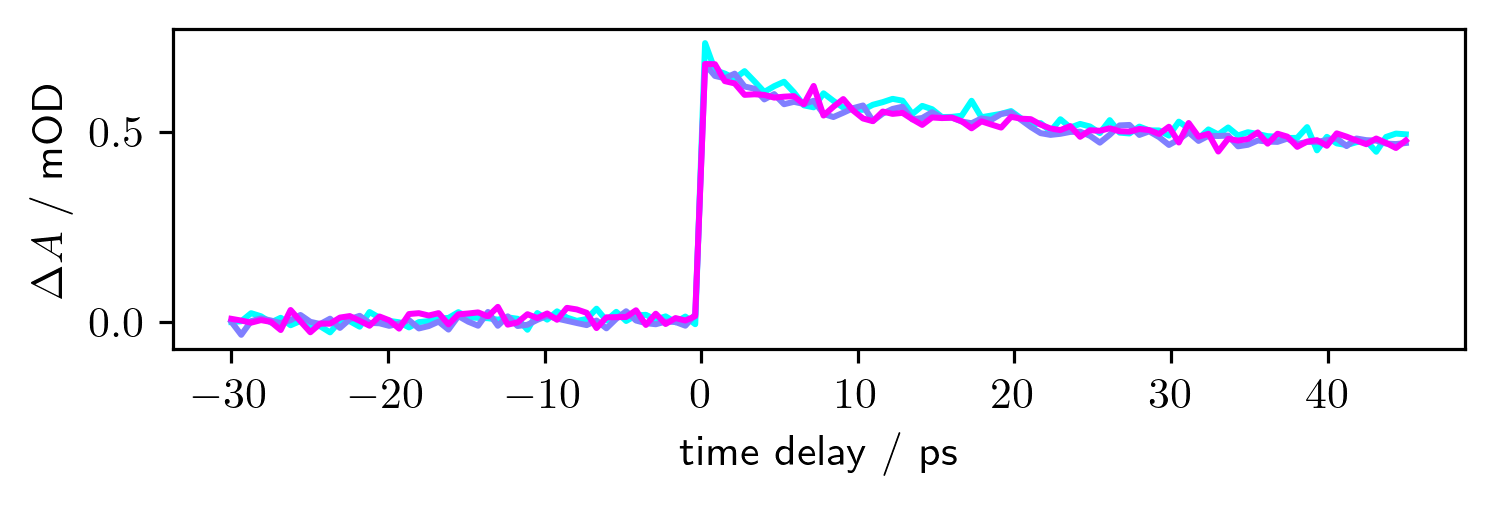
\includegraphics[scale=1]{images/TA_delayscan_493RAW.png}
\caption{Pump \SI{653}{\nano\meter} Probe \SI{493}{\nano\meter} ESA TA\_fourier 6767-6769}
\end{subfigure}
\begin{subfigure}[t]{\textwidth}
\centering
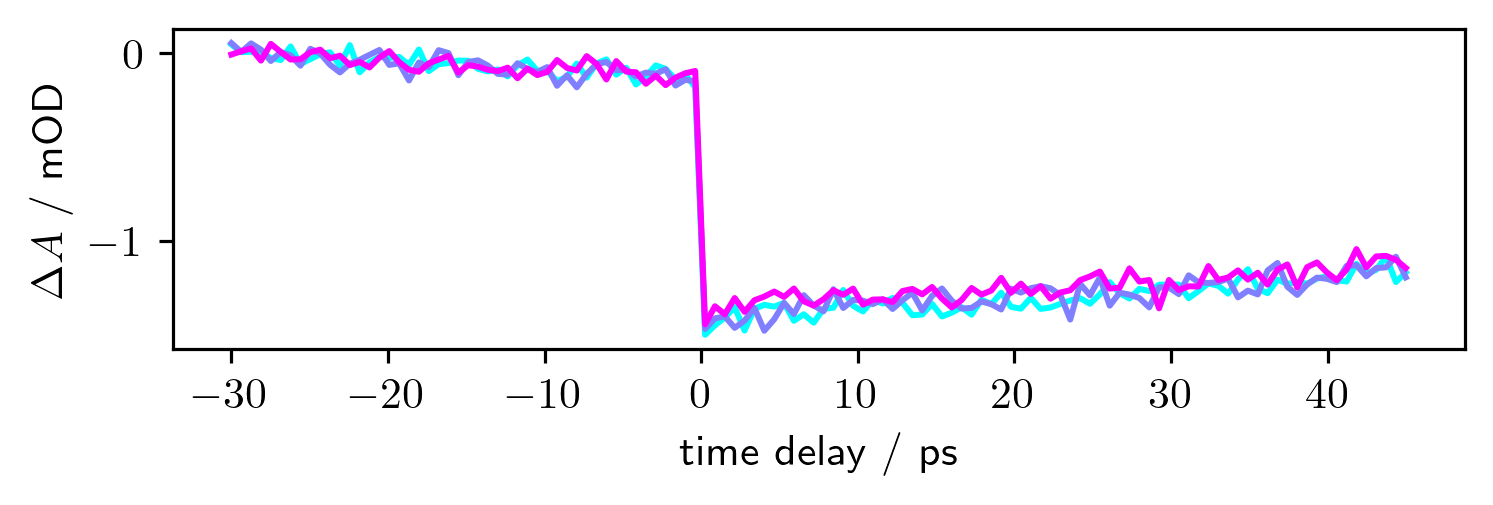
\includegraphics[scale=1]{images/TA_delayscan_680RAW.png}
\caption{Pump \SI{653}{\nano\meter} Probe \SI{680}{\nano\meter} GSD TA\_fourier 6677-6679}
\end{subfigure}
\caption{Examples of measurement series featuring ESA or GSD for 1wt\% SQIB in PMMA\\ Raw measurements without any correction are shown. Each curve is a single measurement belonging to the series plotted in the corresponding figure. Measurements are done in series, thus delay range is scanned for each of the scans.}
\end{figure}


\subsection{Polarization angles}
Pump probe measurements of same polarization obviously return the highest signal in any case. However when working with liquids or (solid) solutions like PMMA in this case the molecules, if relatively unperturbed by the environment, may rotate over time and thus change the direction of their transition dipole moments relative to where they would be in their zero time direction. This leads to a measurable signal change over time.\\
The rotation in the sample is given by the anisotropy at detection:\textbf{find better source}possibly from here\cite{Schalk2010}
\begin{equation*}
r = \frac{I_{\parallel}-I_{\perp}}{I_{\parallel}+2I_{\perp}}
\end{equation*}
where $\mathrm{I_\parallel}$ is the component, where pump and probe are parallel polarizations, and $\mathrm{I_\perp}$ is the component perpendicular to the pump polarization. The reason for the factor 2 in the enumerator is that the original polarization can rotate into two perpendicular directions, which are projected into a direction perpendicular to the pump polarization.???\\
By measuring at the so called "magic angle" of $\theta = 54.7 \degree$ the parallel and orthogonal polarization components are polarized and the measurement is made isotropic. This is based on the transmission of polarized light through a polarizer $I(\theta) = I_0 \mathrm{cos}^2(\theta)$.\\
Alternatively this isotropic output may also be achieved by measuring parallel and orthogonal polarisations and using an arithmetic correction. The total intensity is $I_T = I_x+I_y+I_z = 2\cdot I_\perp + I_\parallel$. To now correct for both rotation directions out of parallel plane the signal may be corrected to $I = \frac{I_\parallel + 2I_\perp}{3}$, which corresponds to the isotropic signal.\cite{Zheng2020}

\textbf{Attempting to plot polarization dependence of simulated molecules rotating, so far does not seem to work like it should}

%Depending on the rate at which the sample decays we should be able to ignore that?
%Our sample is isotropic, so that means we would see, if it was the case that transition dipole of the excited state for the probe was perpendicular to our pump polarization and we still probe parallel to pump, the signal would be rising and still be able to detect if there was a state at that point. Check maybe I have a perpendicular measurement where I can check the rise time, it was relatively quick I remember. Main problem with magic angle is loss of the transient absorption edge, which we like to compare to since we usually use very anisotropic samples.


\section{Squaraines}
Squaraines are investigated for multiple properties making them an interesting model system for organic solar cells. Processing for prototyping is very simple and may be done by spin-coating, such as the samples provided by Manuela Schiek. 

Different crystal structures may be achieved by changing the side-chains or the substrate onto which the crystals are grown. The molecule may be modelled by the semi-empirical essential state model using a simplified electronic representation of the molecule. A donor-acceptor-donor (DAD) structure qualitatively describes the absorption behaviour of unit cells with multiple molecules, which behave as J- or H- aggregates according to the usual Kasha theory depending on their orientation to each other.\cite{Hestand2015}

The stacking and geometry of the unit cell may be tuned by choosing side-chain molecules of appropriate bulkiness. A wide choice of alkyl chain lengths from butyl to octyl, isobutyl and similar molecules that do not directly influence the monomer spectrum are available. However if in crystal configuration through intermolecular charge transfer the absorption spectrum may be changed. \cite{Hestand2015, Brueck2014, Balzer2022}

Theoretical modelling may be done with the semi-empirical essential state model, simplifying the large molecules to a donor-acceptor-donor structure, where the central oxygen groups with high electron affinity act as the acceptors and the nitrogen in the periphery of the molecule as donor.\textbf{who do I quote best?\cite{Zhong2019}} Their crystal structure may be changed by exchanging the length of the sidechains influencing both charge transfer as well as absorption spectra due to shifting of central high electron affinity oxygen to the periphery nitrogen
\begin{figure}[hbtp]
\centering
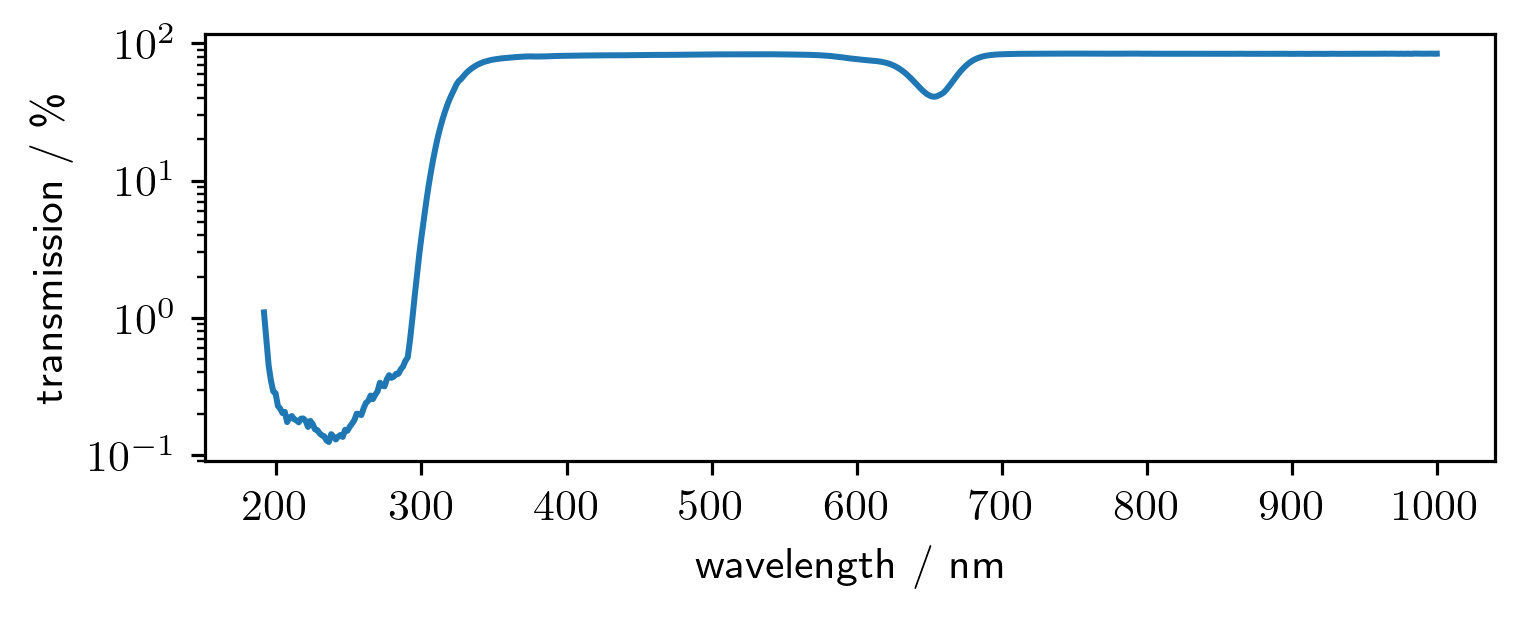
\includegraphics[width = \textwidth]{images/SQIB1percentInPMMA_transmission.png}
\caption{Continuous wave transmission spectrum of the 1wt\% SQIB in PMMA sample provided by Manuela Schiek \textbf{ASK HOW TO REFERENCE THIS}}
\end{figure}

\begin{figure}[hbtp]
\centering
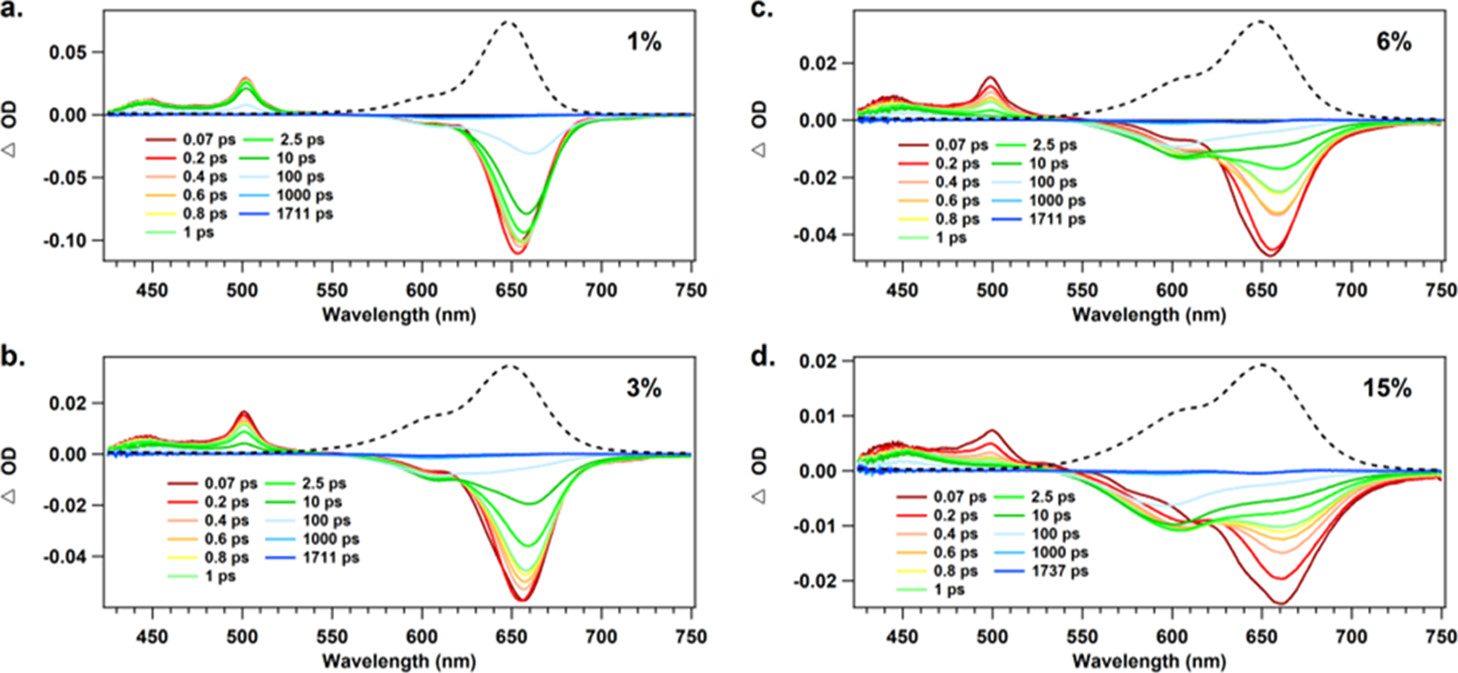
\includegraphics[scale=1]{images/Zheng2020SquaraineTAgraph.jpeg}
\caption{Transient absorption spectra of squaraine with n-butyl sidechains\\
Reprinted (adapted) with permission from \protect\bibentry{Zheng2020}. \\Copyright 2020 American Chemical Society}
\end{figure}


\chapter{Devices and Setup}

Part of the experimental objective was to extend the range of the transient absorption microscope (TAM) into the UV range via SHG of the probe NOPA output. With the extension a wavelength range of 250 nm to 940 nm, with a gap between 470 nm and 500 nm, is available for probing the sample.\newline
To achieve this range a few optics, most notably the achromatic objectives used to image the sample, had to be exchanged for optics non absorbing in the UV.
\section{Regular transient absorption microscope setup}\label{RegTAM}
A short description of the experimental setup for the Transient Absorption Microscope (TAM), as it was before attempting an extension to higher photon energies follows. For further details see previous work by Schwarzl et al.\cite{Schwarzl2022}\\
As a laser source a PHAROS femtosecond laser by Light Conversion is used with an output of 400 µJ at 20 kHz with a pulse length in the range of 270 fs. The output is evenly split between two Orpheus Non-Collinear Optical Parametric Amplifiers (NOPAs), where one is setup with second harmonic (2H) of the Yb-based pump laser (514 nm) for the pump pulses and the other is setup with third harmonic (3H) of Yb (342 nm) for the probe pulses. Some of the NOPA specifications are shown in tab. \ref{tab:NOPAs}. Long term output power stability is mainly important for the pump pulse, which is why the setup, including the compressor the PHAROS, is optimized for maximum stability of the 2H NOPA. Meanwhile having little shot to shot fluctuations is important in all cases. PHAROS is the most reliable part of the setup, with exception of the compression setting which may need adjusting every once upon a while.\\

The NOPAs settings have to be adjusted such that the centroid output, which is controlled via the internal Qmini spectrometer, is on the wavelength intended. The centroid is used as the maximum intensity wavelength may be on the edge of the pulse spectrum. Also note that as seen in fig. \ref{fig:spectrometerMalfunction} the spectrometer data may show periodic intensity variations, which are a device malfunction. Using the centroid avoids strong interference by this type of malfunction. Set wavelength may deviate from output wavelength. In case of low output power resetting motors multiple times may suffice.

\begin{table}
\caption{Specifications of NOPAs used together with the Light Conversion Pharos to pump and probe the sample. Temporal envelope values are from commissioning of the setup. Setup currently is tuned for 2H power stability, which is used to supply the pump pulse.\label{tab:NOPAs}}
\begin{tabular}{lccc}\toprule
Device configuration & wavelength range / nm & photon energy range / eV & temporal envelope / fs \\ \midrule
2H & \SIrange{650}{940}{} & \SIrange{1.32}{1.91}{} & $\leq$ 50 \\ 
2H-SHG & \SIrange{325}{470}{} & \SIrange{1.32}{1.91}{} & - \\\midrule
3H & \SIrange{495}{680}{} & \SIrange{1.82}{2.50}{} & $\leq$ 40 \\
& \SIrange{680}{900}{} & \SIrange{1.38}{1.82}{} & $\leq$ 90 \\
& \SIrange{900}{940}{} & \SIrange{1.32}{1.38}{} & $\leq$ 110 \\
3H-SHG& \SIrange{250}{470}{} & \SIrange{2.63}{4.96}{} & - \\
\end{tabular}
\end{table}

\begin{figure}[hbtp]
\begin{subfigure}[b]{\textwidth}
\centering
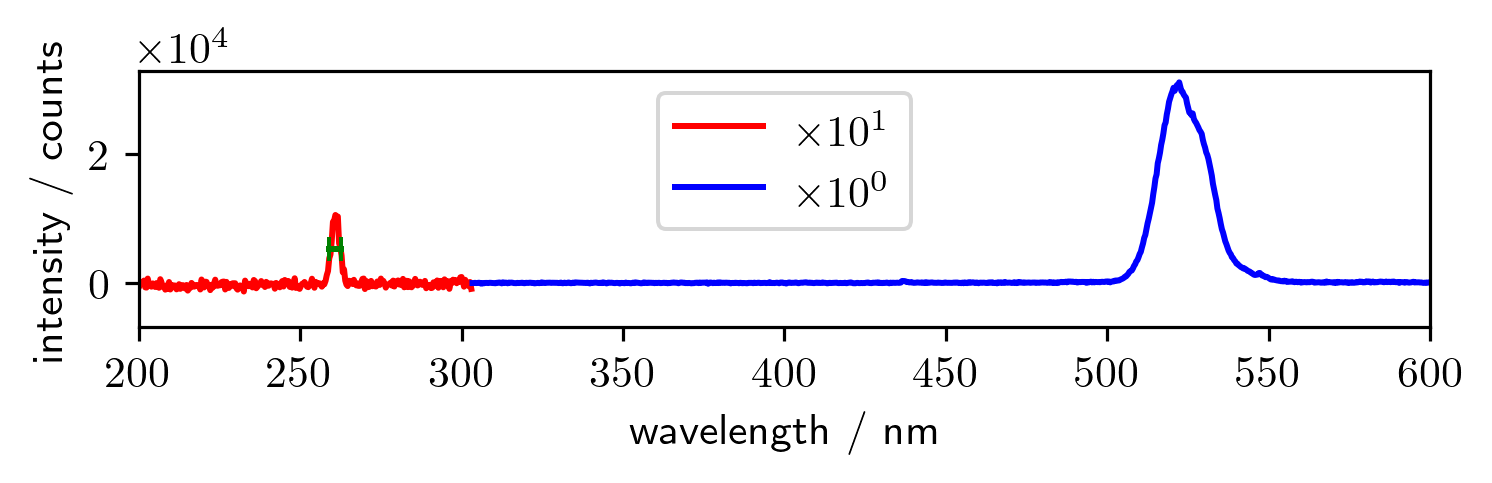
\includegraphics[scale=1]{images/spectra/SpectrumExampleNoFilter_260nm.png}
\caption{Probe FWHM$_{SHG}$ = \SI{3.9}{\nano\meter} Flame spectrometer}
\end{subfigure}
\begin{subfigure}[b]{\textwidth}
\centering
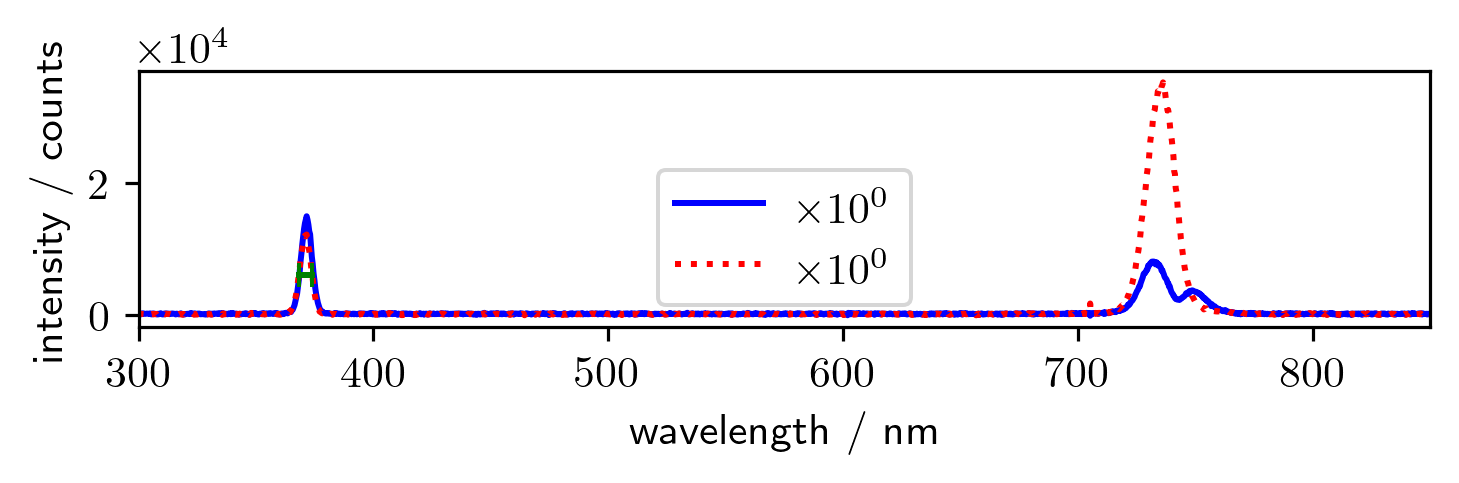
\includegraphics[scale=1]{images/spectra/SpectrumExampleNoFilter_371nm.png}
\caption{FWHM$_{\mathrm{SHG}}$ = \SI{5.6}{\nano\meter}, FWHM$_{\mathrm{fundamental}}$ = \SI{14}{\nano\meter}, Qmini internal spectrometer\label{fig:SHG_offCenterComp}}
\end{subfigure}
\begin{subfigure}[b]{\textwidth}
\centering
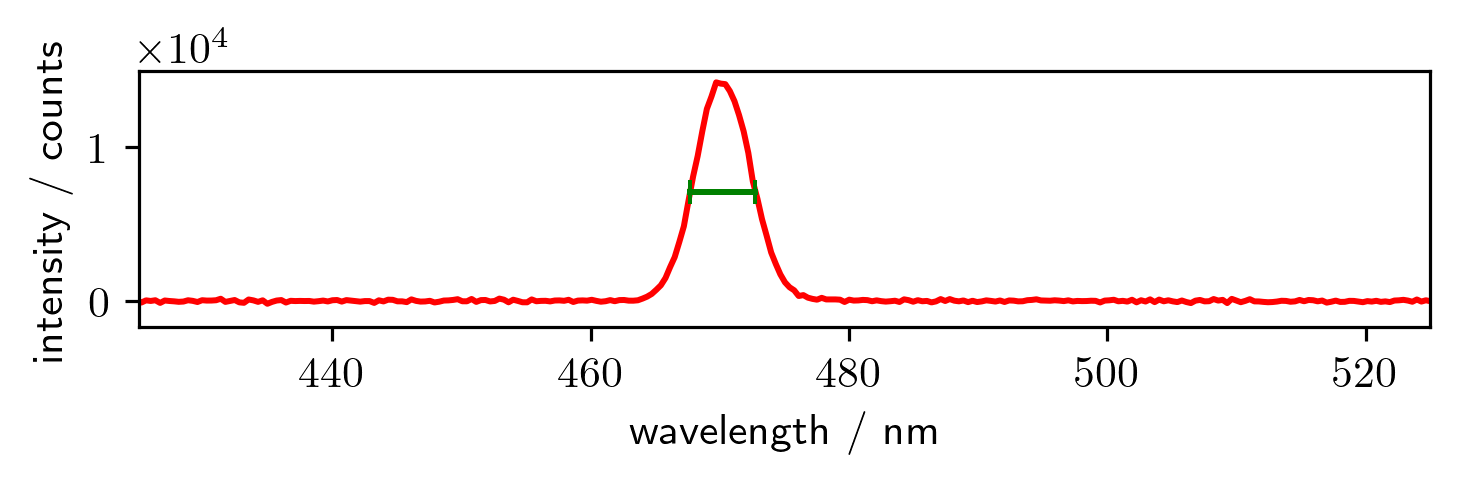
\includegraphics[scale=1]{images/spectra/SpectrumExampleNoFilter_470nm.png}
\caption{Qmini internal spectrometer, FWHM$_{\mathrm{SHG}}$ = \SI{5.1}{\nano\meter}, \textbf{probably discard this one}}
\end{subfigure}
\begin{subfigure}[b]{\textwidth}
\centering
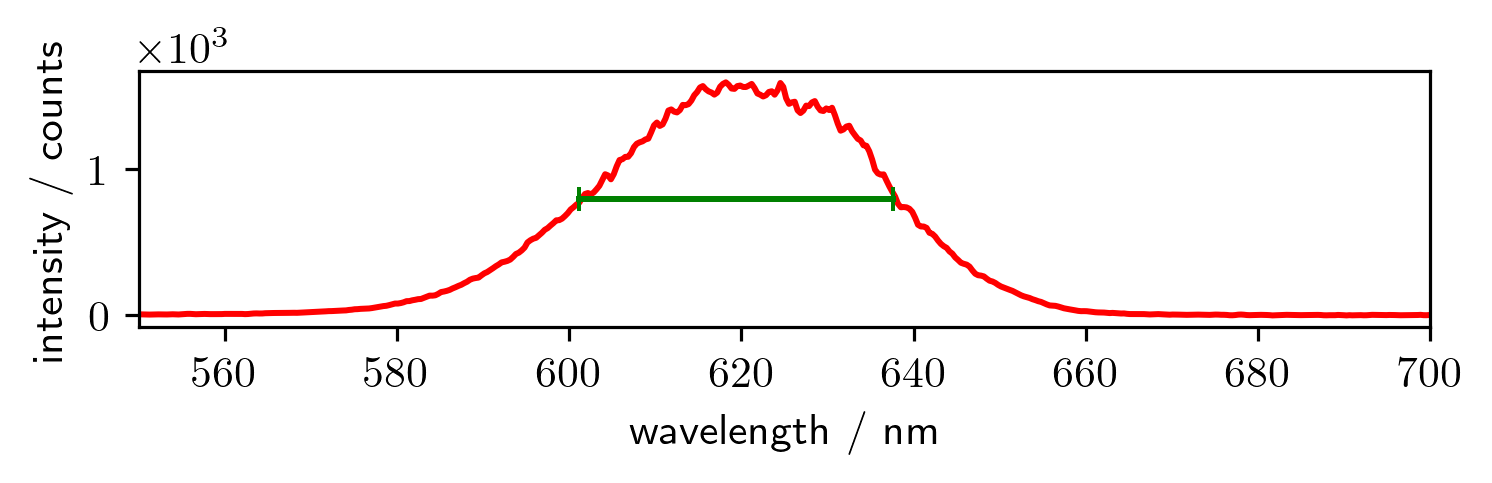
\includegraphics[scale=1]{images/spectra/ActonMonochromatorCharacterisation/620nmSpectrumProbe.png}
\caption{Qmini internal spectrometer, FWHM$_{\mathrm{NOPA}}$ = \SI{36.5}{\nano\meter}}
\end{subfigure}
\begin{subfigure}[b]{\textwidth}
\centering
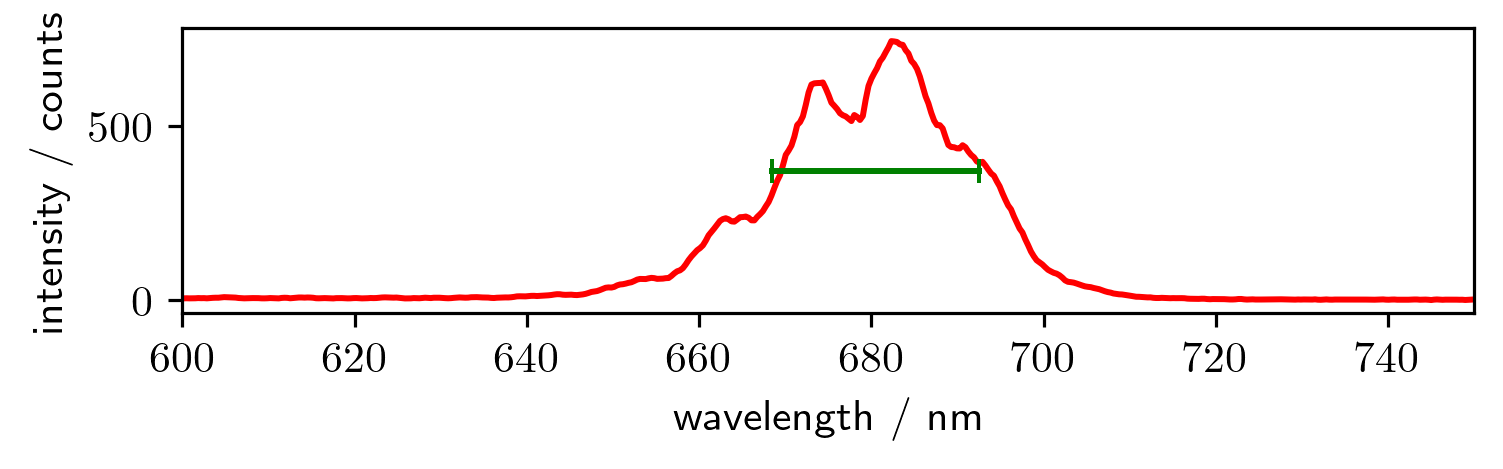
\includegraphics[scale=1]{images/spectra/2024-02-05/probe_3H_680nm.png}
\caption{Qmini internal spectrometer, Spectrometer started modulating intensity as shown periodically. Modulation is consistent. FWHM$_{\mathrm{NOPA}}$ = \SI{24.1}{\nano\meter}\label{fig:spectrometerMalfunction}}
\end{subfigure}
\caption{Examples for spectra used to probe the sample. FWHM is calculated with Waves.\label{fig:probeSpectra}}
\end{figure}

\begin{figure}[hbt]
\centering
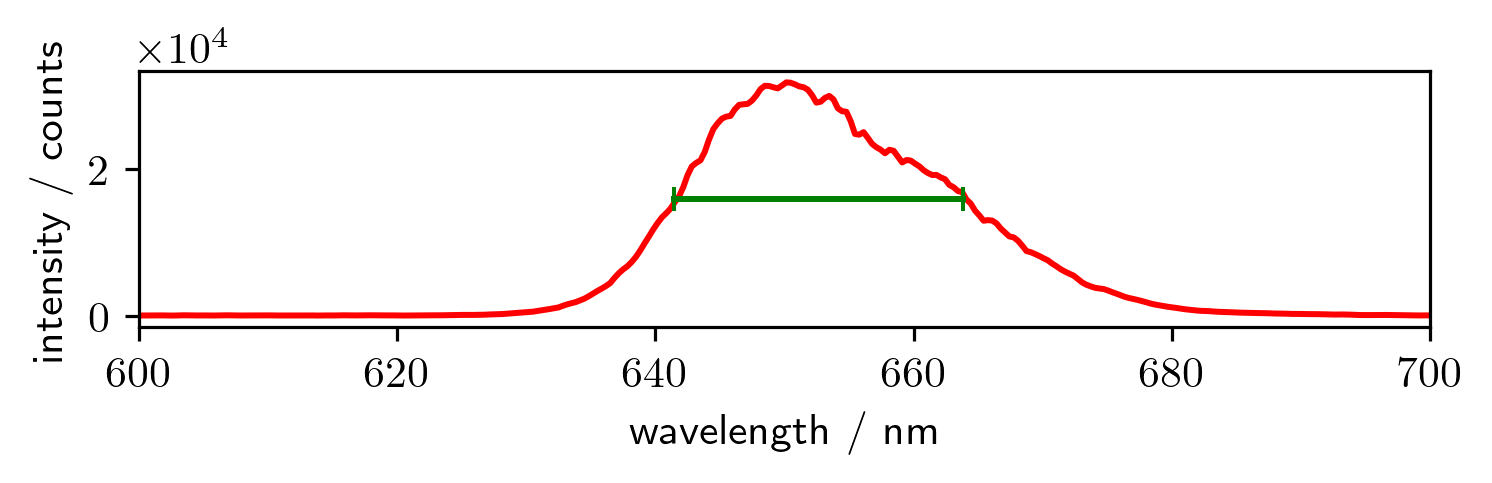
\includegraphics[scale=1]{images/spectra/2024-02-05/pump_2H_653nm.png}
\caption{653 nm pump as used for measurements, Qmini internal spectrometer, FWHM = \SI{22.4}{\nano\meter}}
\end{figure}

The light following the pump path goes through several apertures and ND filters, which may be absorptive glass filters or metal coated reflective filters which may also be gradient filters for linear adjustability, until the beam reaches the linear delay stage, which uses a Newport LTA-HS actuator. The beam path is then led through the chopper by the use of a roughly 1:1 telescope around it, which blocks every second pulse leaving a half frequency signal for the pump. The chopper is synchronised to a signal output of PHAROS, which allows for setting a delay such that there is just a binary on and off modulation of the pump, compared to a partial chopping of beams at full frequency. After passing through a lambda half wave plate the beam enters the common path in the cage with the sample.

The probe beam has the same treatment of apertures and ND filters, including a variable reflective one, and goes through a $\mathrm{\lambda/2}$ plate until it reaches the common path.


For detection of the transient signal a custom made detector based on Hamamatsu S1336-8BQ Si photodiode is used in combination with an analogue long pass amplification circuit stretching the signal such that it can be measured with a picoscope 5442D. For all measurements detector "A" was used. The diode is fit for measurements in the wavelength range of 190-1100 nm. The actual quantum efficiency change over the spectral range does not matter in detail, as the variation over the spectral range is slow and for the spectral range of a probe setting does not exceed 10\% change at any point.

\section{UV extended transient absorption microscope setup}
This section will address the issues addressed with the extended setup as well as attempted solutions and the final changes to make it work.

\begin{figure}[h]
\centering
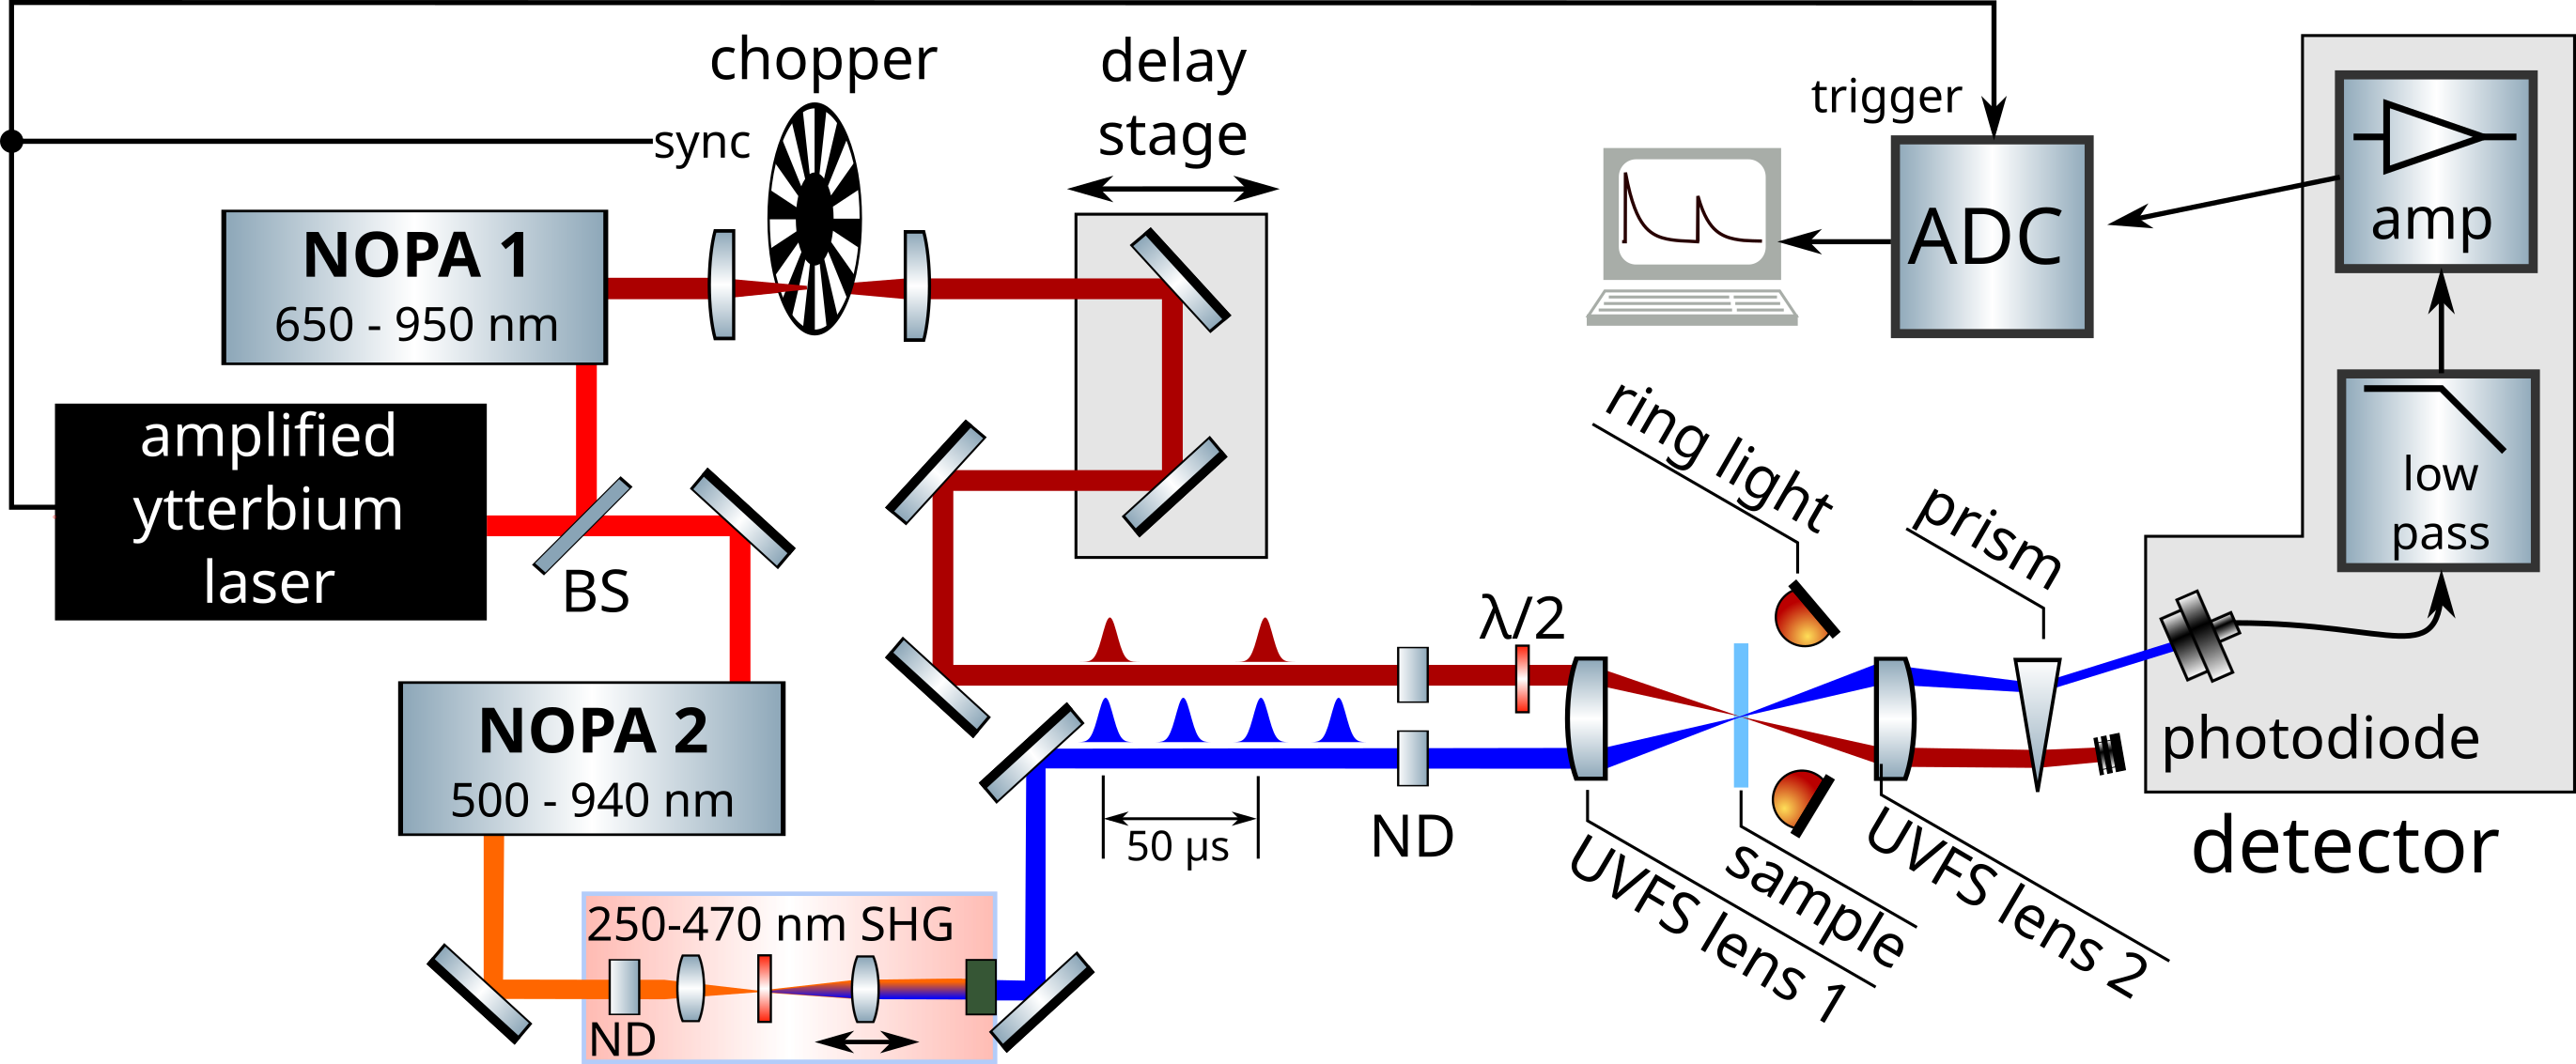
\includegraphics[width=0.9\linewidth]{images/ComponentLibrary_svg/experimental_tam_shg_swapped.png}
\caption{UV extended TAM\\Pump adjustable for 650 nm to 940 nm
\\Probe adjustable between 500 nm and 940 nm with the option of separate range of 250 nm and 470 nm via SHG crystal\\
SHG stage shown including optional filters to remove white light from NOPA (ahead of SHG crystal) and fundamental wavelength of SHG (after SHG crystal)\\ Cage setup in further detail in fig. \ref{Fig:CageSetup}}
\end{figure}

\begin{figure}[h]\label{Fig:CageSetup}
\centering
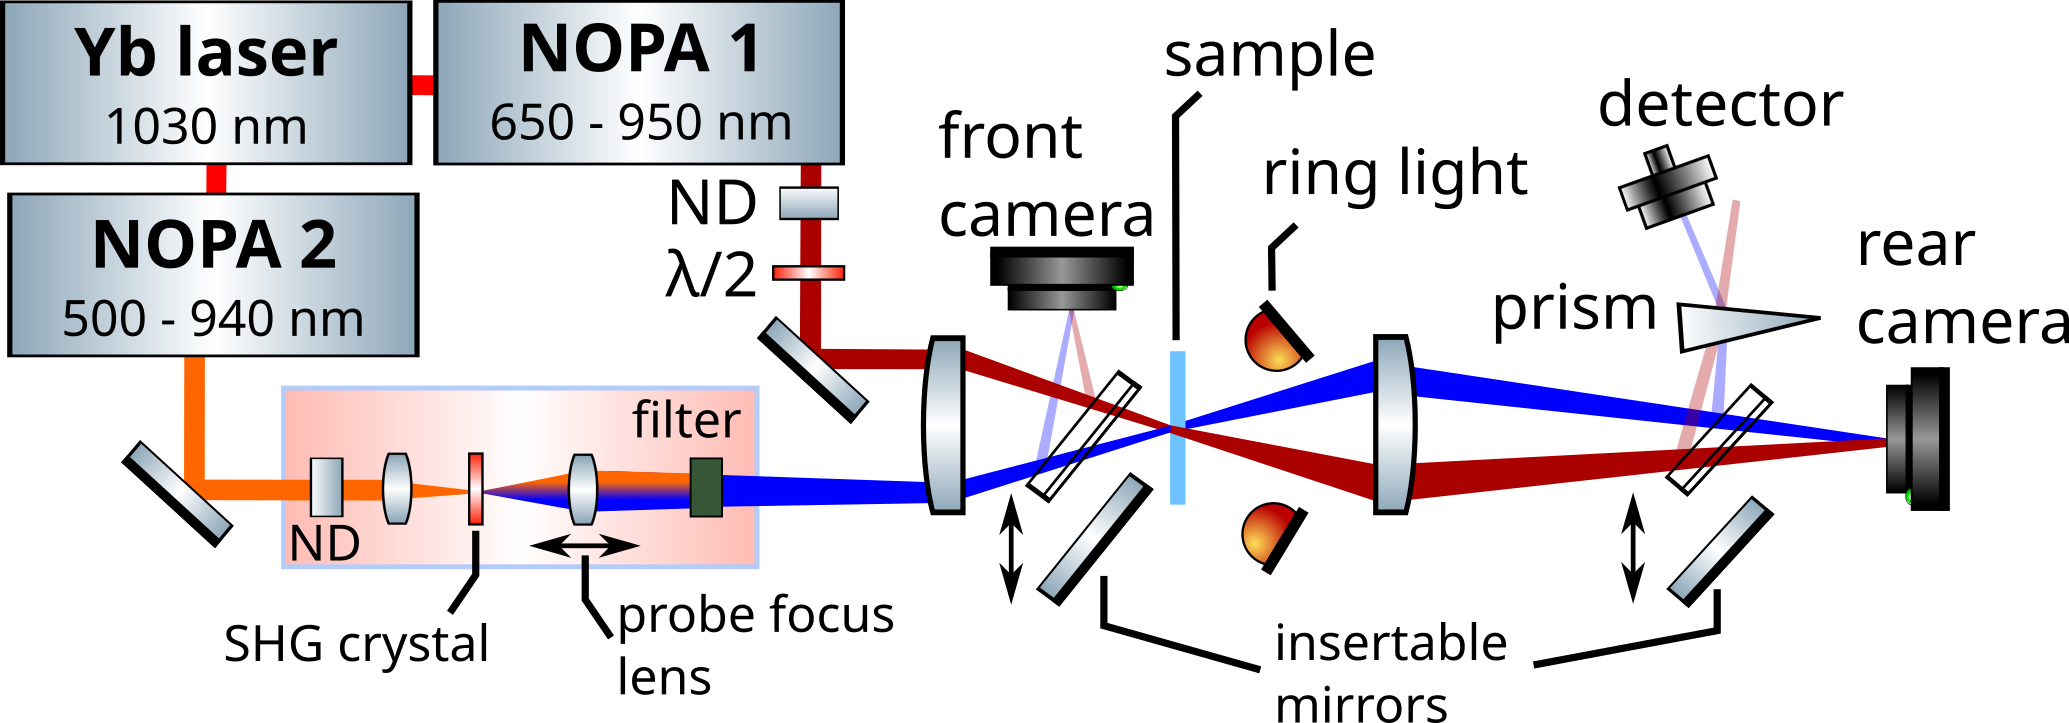
\includegraphics[width=0.9\linewidth]{images/ComponentLibrary_svg/SHG-focusing-large.png}
\caption{Detail view of new components in TAM\\ Ahead of first show probe lens white light remainder from NOPA may be filtered and after the second lens the fundamental may be filtered\\
Rear camera shown as coupled out of the standard path, however it is advised to instead have the rear camera in the standard detector path and only insert the mirror coupling into the mirror when doing measurements.}
\end{figure}

\subsection{Cage setup}
To accommodate the lower wavelengths the objectives have to be exchanged for wavelengths below 350 nm, where absorption reduces the transmission of the objective combination severely. Furthermore only one of the objectives is rated down to 350 nm raising the question of if their achromacity still is a viable assumption.\newline
The objectives are replaced with  uncoated 125 nm plano-convex UV fused silica (UVFS) lenses from EKSMA\footnote{?110-1216E?}, with the convex side placed such that the collimated beam enters or exits the convex side. This means that the planar sides of the lenses point towards the sample as can be seen in fig. \protect\ref{Fig:CageSetup}. This is done to reduce spherical aberration.
\newline
The plano-convex lenses are neither apochromatic nor achromatic and thus exhibit chromatic aberration, leading to an issue that will be addressed in sect. \ref{SHG-Stage-desc}. \newline

\subsection{Second harmonic generation stage}\label{SHG-Stage-desc}
The Second Harmonic Generation (SHG) stage addresses multiple issues. 
\begin{itemize}
\item The 3H NOPA used for the probe beam does not supply high enough power to allow for stable SHG over the entire output wavelength range of the NOPA without a focusing element increasing the power locally within the crystal. 
\item The chromatic aberration or focus shift within the cage system means that a degree of freedom on the focus of the probe needs to be included as to allow adjustments to the point spread function of the probe.
\end{itemize}


The solution to these issues is an adjustable telescope of biconvex lenses, of which the second lens has to be UV transmissive. To achieve a stable second harmonic generation (SHG) a telescope was built with two spherical lenses. The front lens is a 85 mm lens in a mount adjustable for horizontal and vertical displacement orthogonal to the beam path and the rear lens is a 75 mm UVFS lens on a linear stage, to provide a degree of freedom for the focus of the probe beam, which is necessary to account for the achromacity of the extended setup. The SHG crystal position and input fundamental power have to be adjusted by hand for every wavelength. An example for a SHG spectrum along with its fundamental is shown in fig. \ref{fig:specSHG300nm}. Note how the fundamental peak is missing intensity off center. The SHG wavelength is given by the phase-matching condition, thus there is some uncertainty in the SHG center wavelength if no spectrum is recorded, as usually done here. Due to SHG being a $\xi^{\left(2\right)}$ process it is quadratic in power regarding fundamental field strength limiting this center wavelength shift to the half value positions of the fundamental for this use case, as SHG intensities are kept only as high as needed. For the measurements presented in chapter \ref{chpt:results} the maximum shift likely is even more limited, as only the spectrum very close to the maximum intensity wavelength leads to good output intensity for relatively low powers. An off center SHG phasematching condition may be seen in fig. \ref{fig:SHG_offCenterComp}, where both graphs have the same wavelength SHG output, however the the fundamental wavelength of the red graph is shifted below double the SHG wavelength. \textbf{read up in labbook 01.09.2023}
\begin{figure}[hbtp]
\centering
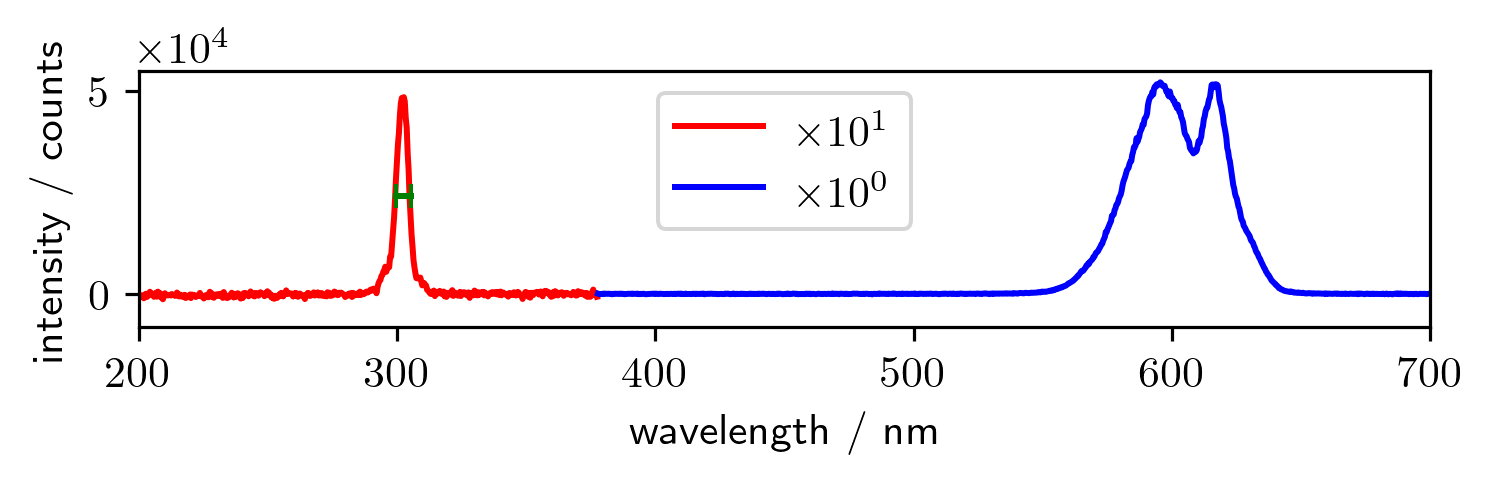
\includegraphics[scale=1]{images/spectra/SpectrumExampleNoFilter_300nm.png}
\caption{600 nm fundamental SHG\label{fig:specSHG300nm}\\ FWHM$_{SHG}$ = \SI{6}{\nano\meter}}
\end{figure}
\subsubsection{Operation}
\paragraph{Setting up}
The task of setting up the SHG stage is non trivial regarding proper alignment and linear stage positioning, such that the ~5 cm of movement are sufficient to adjust for the chromatic aberration within the targeted wavelength range for probe. This task often ends up being trial and error in correspondence to checking multiple wavelengths. The cage lenses have to be in their correct positions first.\newline
Irises etc are beneficial if there is a working setup.\newline
Use irises to shape the probe beam to an acceptable Gaussian shape while avoiding diffraction effects. Optimally the incoming beam is level with the table, since any inclination will introduce an \textbf{astigmatism?} depending on the rear lens position.\newline
Begin with the first lens in the path leaving enough space for the linear stage and the SHG crystal to the next static optic. Set lens centered regarding beam. Use the irises in front of the lens to adjust the reflection on the lens surface to return the exact incoming beampath.\newline
Place the rear stage lens and once again adjust for center position. One may again use the reflection and additionally the transmitted beam to tell if the stage is parallel to the beam path. The center of the beam should not move when translating the stage and the expansion of the beam diameter should be as symmetric as possible. Adjusting via the reflection is not such a clear indication of alignment here, as there are multiple convex surfaces in play at this point, leading to multiple focal beams, what may not be in full accordance with each other. For this usually it was chosen to get the highest intensity spot, which refers to the final glass/air surface of the second lens, in the incoming beam path. This spot is also focused, which makes adjustment easier.\newline
Finally one can adjust mirrors after the stage to get an image on the camera again, as even relatively minute changes in alignment will lead to some beam offset and change in direction. Translating the stage then will give an indication of how well the SHG stage is set up in regards to astigmatism which can be seen as non symmetric expansion of the beam. However beware that the mirror outcoupling in the cage also influences the way a change in focus is experienced, due to deviations from an orthogonal inclination angle to the sensor.




\paragraph{For measurements}
To find SHG intensity approach from the incoming beam direction and adjust SHG crystal until sufficient output power is achieved.\newline
Adjust the linear stage such that there is no lateral movement. The current stage slide is mounted in a way that can rotate a bit if force is applied at the corners. It may be necessary to do this and have the stage "snap back" to make sure it will not move during the measurement. This can be checked after the measurement by checking the overlap again.\\
Schott glass filters may be used to reduce the intensity of the fundamental wavelength. In some cases interferometric mirrors may be needed to remove background from the NOPA. The increased temporal pulse-length is acceptable due to the long lived nature of the excited states of the sample used. internal transmittance spectra of the filters used, which in some cases may be combined, are shown in fig. \ref{fig:SchottFilters}.

\begin{figure}[hbtp]
\centering
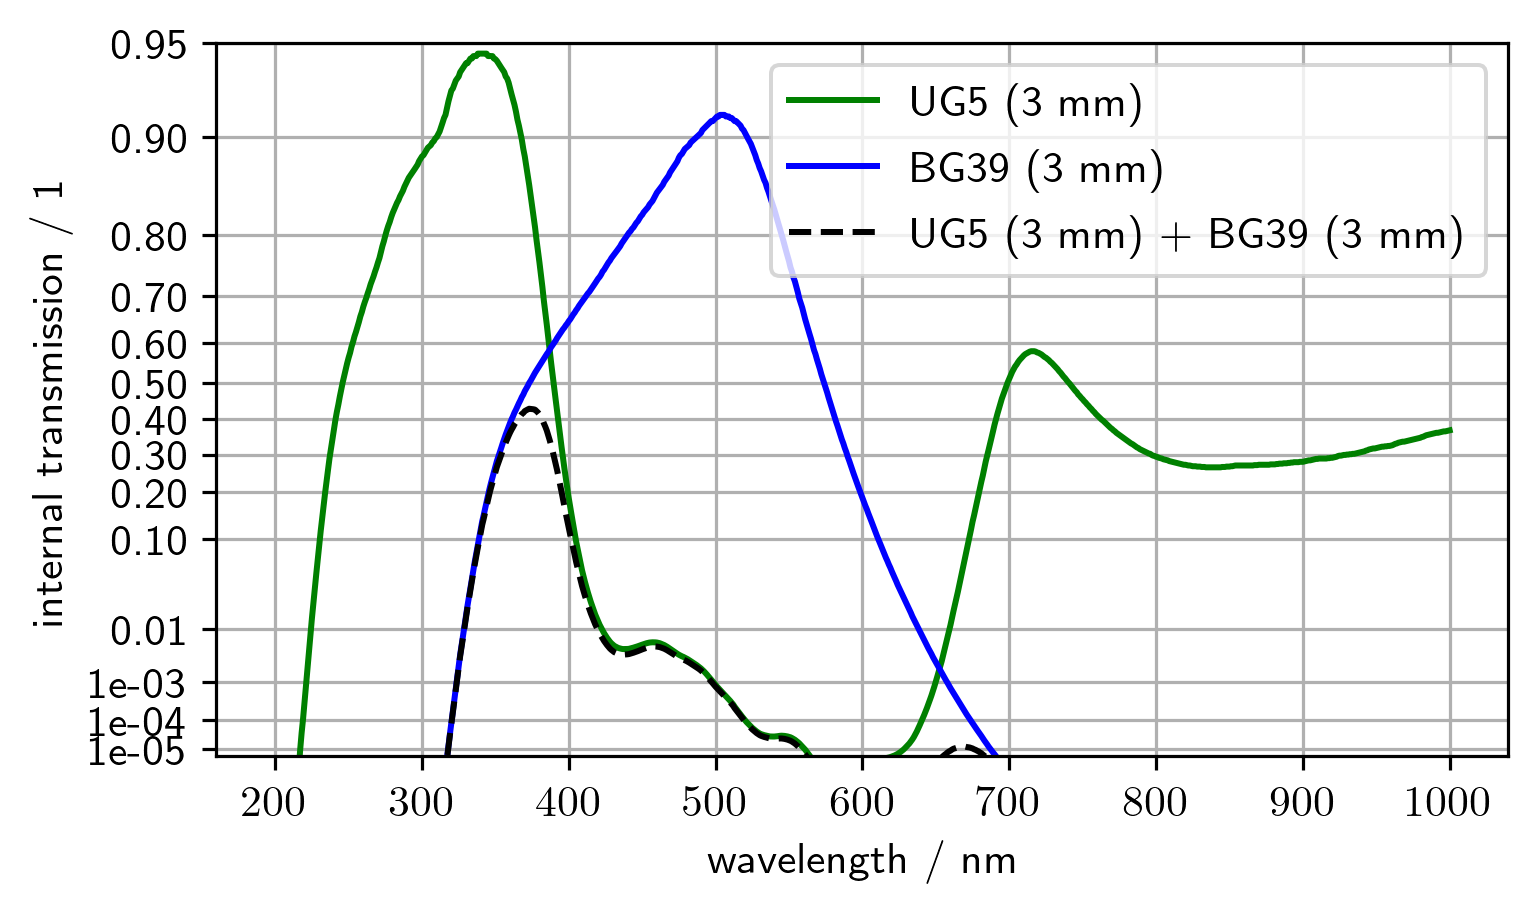
\includegraphics[scale = 1]{images/SchottFiltersFromTool.png}
\caption{Internal transmittance of Schott glass filters in 3 mm used for fundamental filtering.\label{fig:SchottFilters}}
\end{figure}

Alternatively to using glass filters a polarizer may also be used. Reasoning is that for the BBO only type 1 phasematching is possible with a singular fundamental polarized beam, where the fundamental polarization (ordinary polarization) is orthogonal to the SHG output (extraordinary polarization). Note however that the wire grid type polarizer has a falling external transmission and falling extinction ratio for low wavelengths in the UV. Thus mainly the fundamental intensity is modulated with rotation of the polarizer.

\subsection{Detector setup}
The detectors themselves are the same as described in Schwarzl et al.\cite{Schwarzl2022} Matlab software for the measurements was devised by Pascal Heim. For the measurements detector A was used at all times in combination with a picoscope 5442D. An isosceles, UV translucent, prism is inserted to remove any remainders of the fundamental probe wavelength at the detector. To improve this separation an extra iris may be used immediately in front of the detector.\\
The prism should be placed such that the angle between pump and probe is further increased, as this can help reach full pump rejection without any other filters or beamblocks involved. For each change of the probe the mirror coupling into the prism should be adjusted for maximum intensity of the probe on the detector, which can be monitored using the fourierDetector() matlab program.\\
The detector has a maximum peak to peak voltage (Vpp) of approximately 3 V, which means that the Vpp should be kept below this value to avoid response problems and thus systematic errors in the measurement.
\subsection{Adjusting overlap without achromatic optics}

\subsubsection{General overlap adjustment}
Overlap adjustments are done using a camera onto which the sample plane is imaged. This is combined with a fitting program, which fits a Gaussian point spread function to the beam image. From this a center position as well as the FWHM of the point spread function can be determined and used to move the point spread functions on top of each other. The detailed software explanations and their use is explained in chapter \ref{chp:Software}.\\

\paragraph{The problem of achromatic optics}
One of the main issues that had to be addressed was the change from achromatic objectives to uncoated plano-convex lenses within the cage.\newline
This is emphasized especially by plotting the wavelength dependence of the focal length, see fig. \ref{fig:ChromFocalShift} , as defined by the lensmaker equation for the lenses used:
\begin{equation}
\frac{1}{f} = (n-1) \left[\frac{1}{R_1} - \frac{1}{R_2} + \frac{(n-1)d}{n R_1 R_2}\right]
\end{equation}
\begin{figure}[h]
\centering
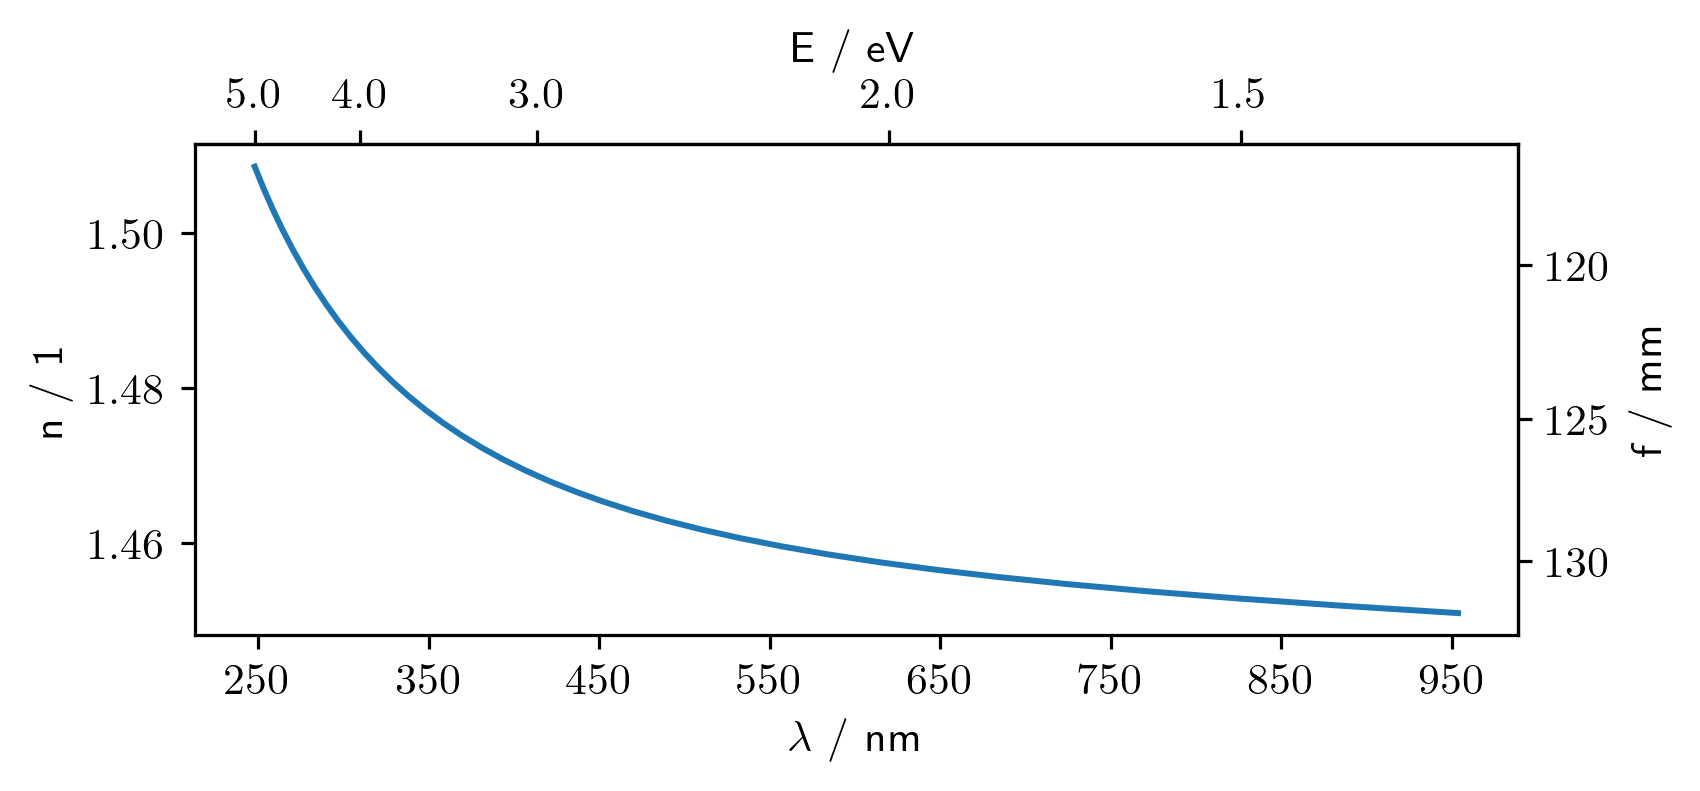
\includegraphics[scale = 0.5]{images/ChromaticFocalShiftandDispersionUVFS.png} 
\caption{Refractive index change and focal shift for UV fused silica plano-convex lenses used in cage setup\cite{Malitson:65}\label{fig:ChromFocalShift}}
\end{figure}

Furthermore the depth of focus may be visualized by plotting the beam waist diameter over distance from the focal point for several relevant focal lengths in fig. \ref{fig:beamWaistCompendium}. The change of the depth of focus (DOF) and thus the change in beam waist diameter for a specific distance from the focal point of the corresponding wavelength decreases for higher photon energies.

\begin{figure}[h]
\centering
\begin{subfigure}[t]{0.49\textwidth}
\centering
\includegraphics[scale=1]{images/BeamWaist_Wavs_2.5mm.png} 
\subcaption{Beam waist for wavelengths at \mbox{2.5 mm} input beam diameter}
\end{subfigure}
\hfill
\begin{subfigure}[t]{0.49\textwidth}
\centering
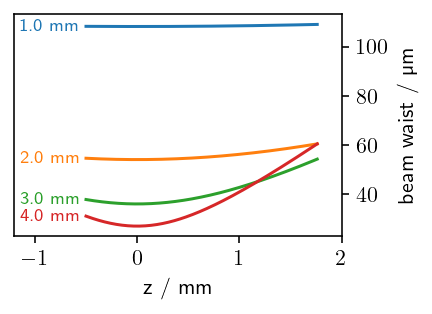
\includegraphics[scale=1]{images/BeamWaist_inputWidth_653nm.png} 
\subcaption{Beam waist for several input beams diameters at 653 nm}
\end{subfigure}
\hfill
\\
\centering
\begin{subfigure}[t]{\textwidth}
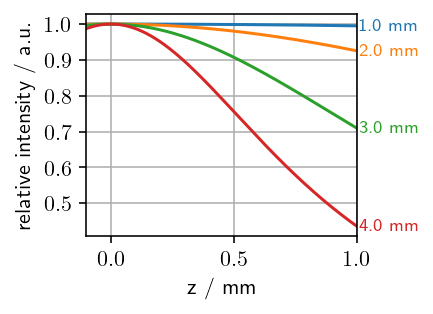
\includegraphics[scale=1]{images/DOFintensity_inputWidth_653nm.png} 
\subcaption{Maximum radiance intensity relative to maximum intensity in focus depending on input beam width at 653 nm \textbf{[check if this assumption is correct]}}
\end{subfigure}
\caption{Changes of simulated Gaussian beam profile width and intensity for lenses used in the cage system, EKSMA 110-1216ET with 125 mm focal length at 355 nm, over distance z from focus. Assuming perfect Gaussian input beam. \label{fig:beamWaistCompendium}}
\end{figure}

This issue is of fundamental nature and a few attempts were made until the following solution was found:

\subsubsection{Sample mirror path}\label{SampleMirrorCamera}
The option that finally won out is decoupling the beams after the frontal cage lens and imaging onto a camera that is in the mirror plane of the sample surface. This method requires a process for consistent placement of the mirror within the cage and a way to move the camera into the mirror plane of the sample.\\


\paragraph{Calibration method}
The rear lens is set to image the sample plane onto the camera as described in \ref{regRearFocus} with a pump adjacent wavelength used to illuminate the sample from the detector side, which amounts to back illumination for the rear camera. This is done to be able to use the pump beam as a reference for the cage system, as the front focus for the sample and the rear focus for the rear camera are both calibrated using a wavelength with very little chromatic focal shift from it.\\
A two step process is then used to get the position of the front camera, in the mirrored sample path, correct:
\begin{enumerate}
\item It may seem like a good idea to just minimize the beam waist of the imaged pump beam. However due to effects of the inversion on fitting this does not work strictly. \textcolor{red}{Adjust the frontal camera distance so, that the pump beam profile is right before inversion, due to passing through the focal point. Inversion being the outer features of the beam profile passing through the center. The intensity still rises a tiny bit beyond that point.} Attention has to be paid to not go into inversion, which is hard to tell by eye. After a first good calibration this could be done by comparing the fitted intensity value/FWHM of the beam profile, as long as the pump beam path did not change. Placement of OD filter in front of camera or in front of cage does matter, swapping the position changes the beam profile. This is due to a change in optical path length due to the different refractive index of the OD filter.
\item Set the probe to the same or an adjacent wavelength to the pump and setup overlap using the rear camera. Due to beampaths and thus spherical aberration this may be a tedious process and not completely accurate. Check the overlap on the frontal camera by moving the camera back and forth and observing if the beams cross through their centers. If that is the case the pump probe overlap should be given optimally and the frontal camera can be set to the optimum position of this overlap. Take reference TA measurements if possible to check if there is an improvement from the purely rear camera based position.
\end{enumerate}

\textbf{Why is the resulting um/px not identical to the 5.6 $\mu$ pixel size? Can I use this to further estimate errors?}
\paragraph{Setup}
Former is solved by a 45 degree mirror insert for the cage, which was designed to rest on top of the cage system rails. This drop in mirror mount was 3d printed for adjustability and has proven to be consistent enough to allow for this method to work. \\
An advantage of PLA as opposed to aluminium with the negative of the rails cut into it is that its mechanical compliance allows proper sliding into place, whereas aluminium "gripped" onto the rails making it hard to get consistent placement. This may be improved by cutting the rail negative in aluminium even slightly larger. However this still presents one with the problem of how to mount the mirror to the mount. Super glueing  the mirror to a aluminium mount was attempted for a quick trial, but this proved to not be a long lived connection.\\
\begin{figure}[hbtp]
\centering
\begin{subfigure}[t]{0.66\textwidth}
\begin{subfigure}[t]{0.45\columnwidth}
\centering
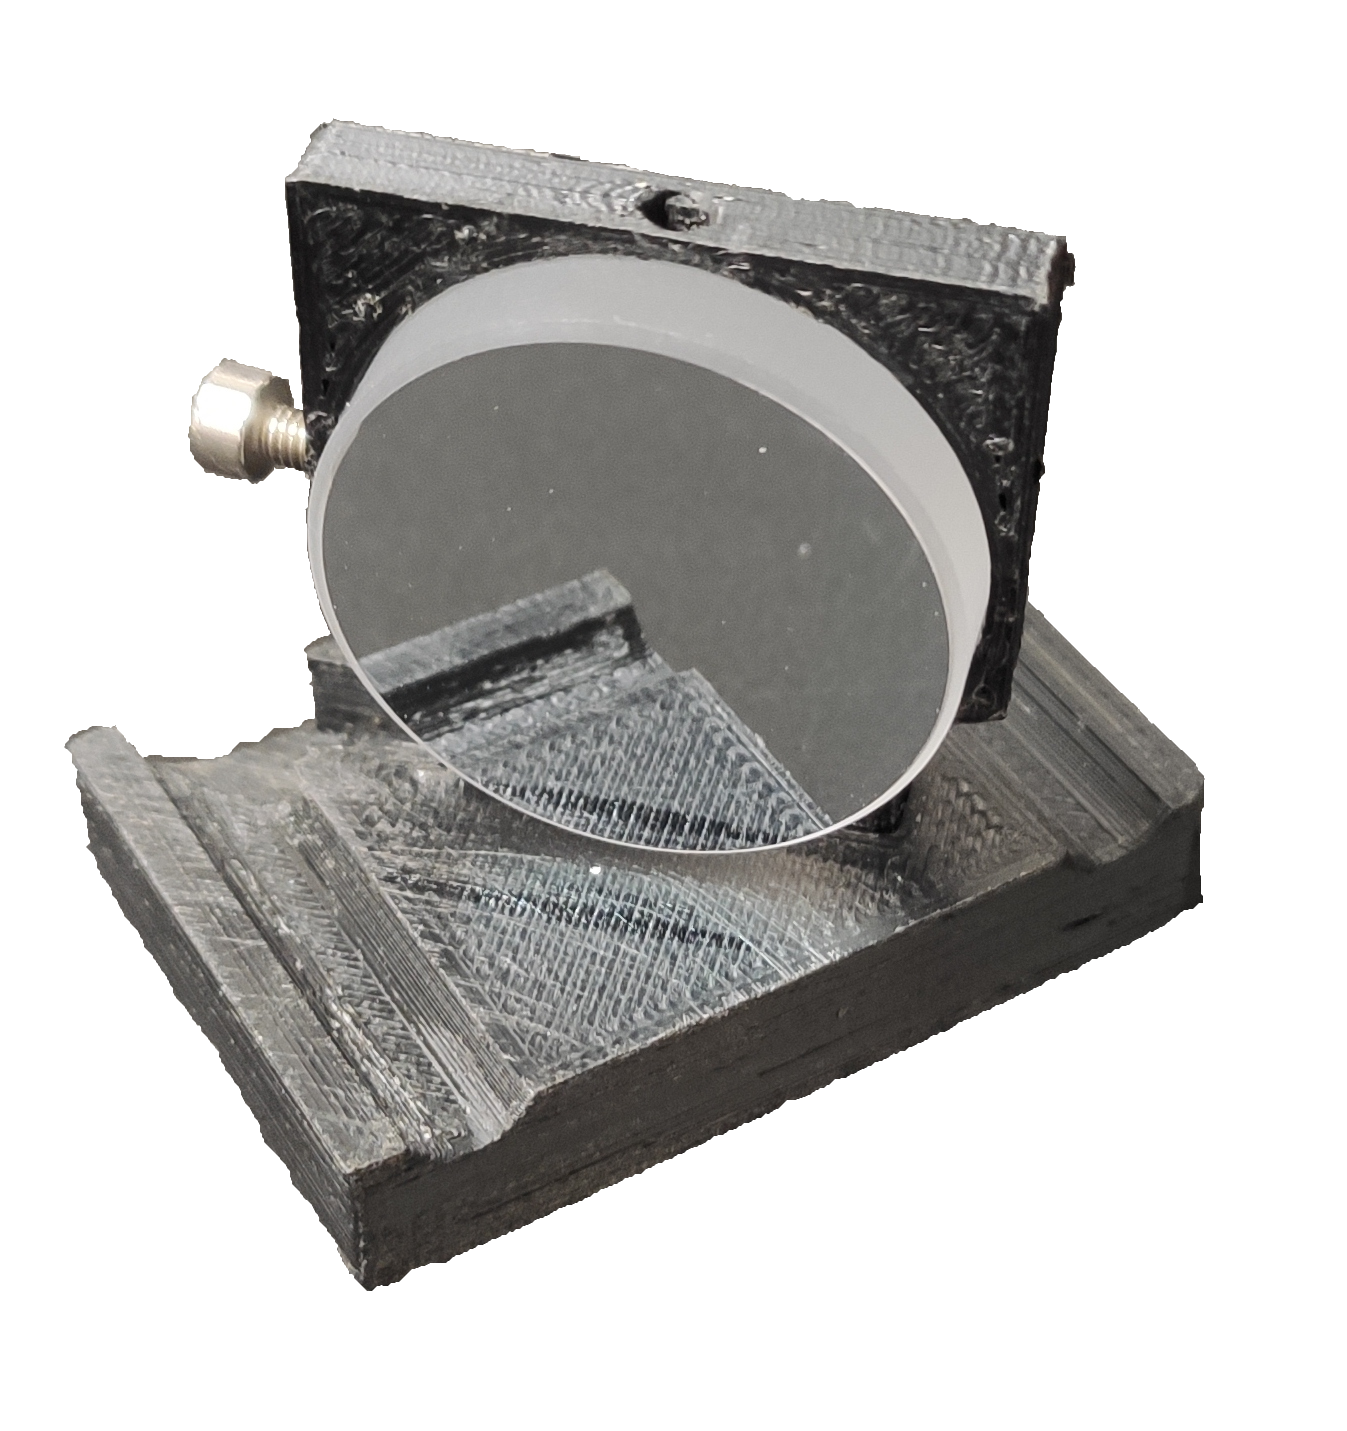
\includegraphics[width=\columnwidth]{images/TAM/MirrorDropInFrontFree.png}
\end{subfigure}
\hfill
\centering
\begin{subfigure}[t]{0.45\columnwidth}
\centering
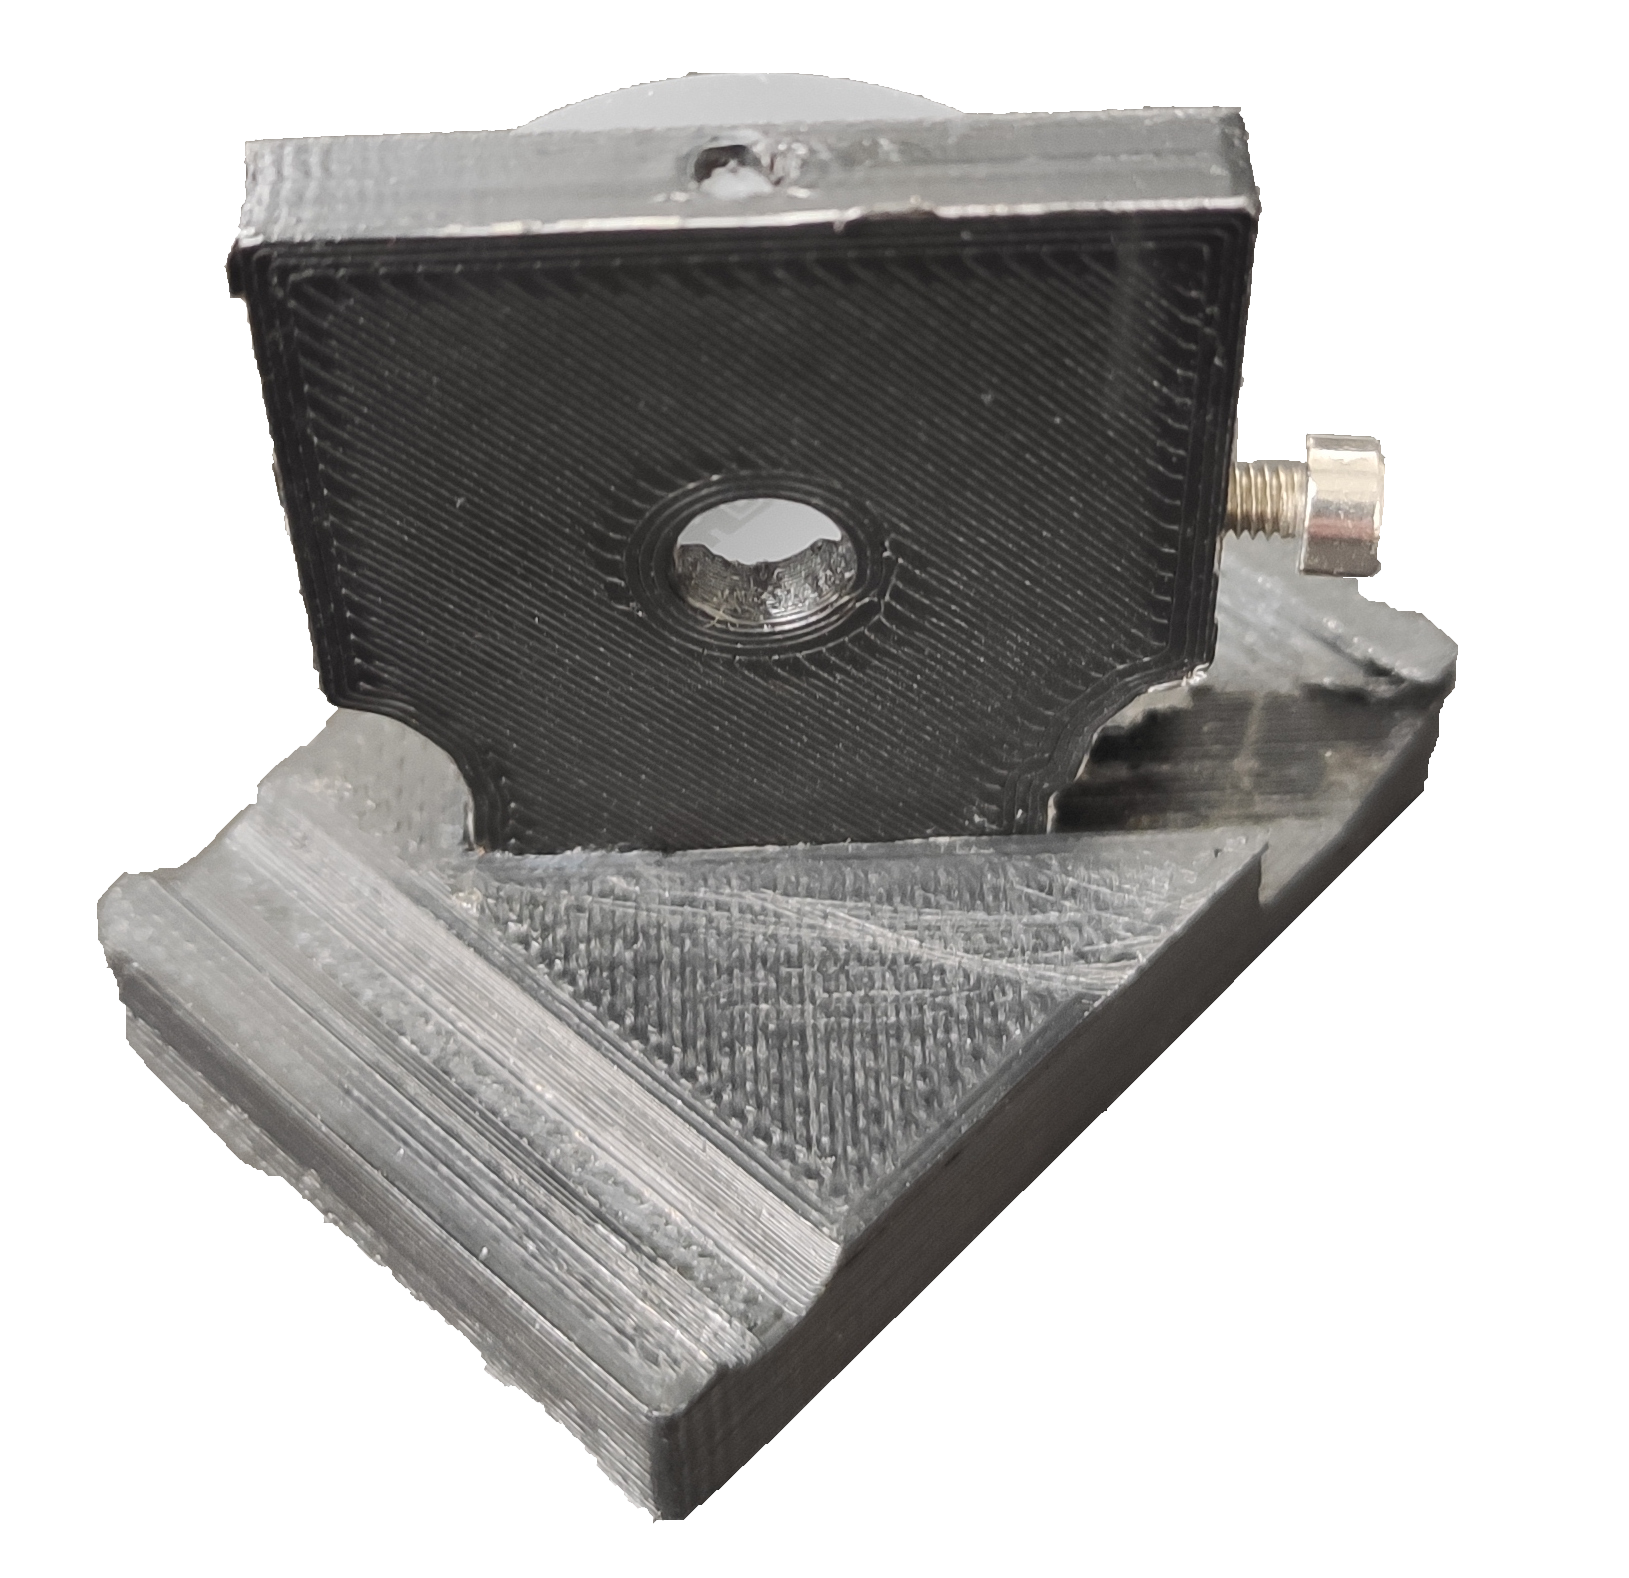
\includegraphics[width=\columnwidth]{images/TAM/MirrorDropInBackFree.png}
\end{subfigure}
\caption{3d printed drop-in mount with mirror\\
The mount is designed for use with 30 mm cage systems like the Thorlabs system and may be parametrically adjusted.
It is printed in two parts, which use joinery to interlink and are fixed together with super-glue to avoid movement.
The mirror may be attached via a friction fit and a flat screw.\label{fig:drop-in-Mirror-mount}}
\end{subfigure}
\hfill
\centering
\begin{subfigure}[t]{0.3\textwidth}
\centering
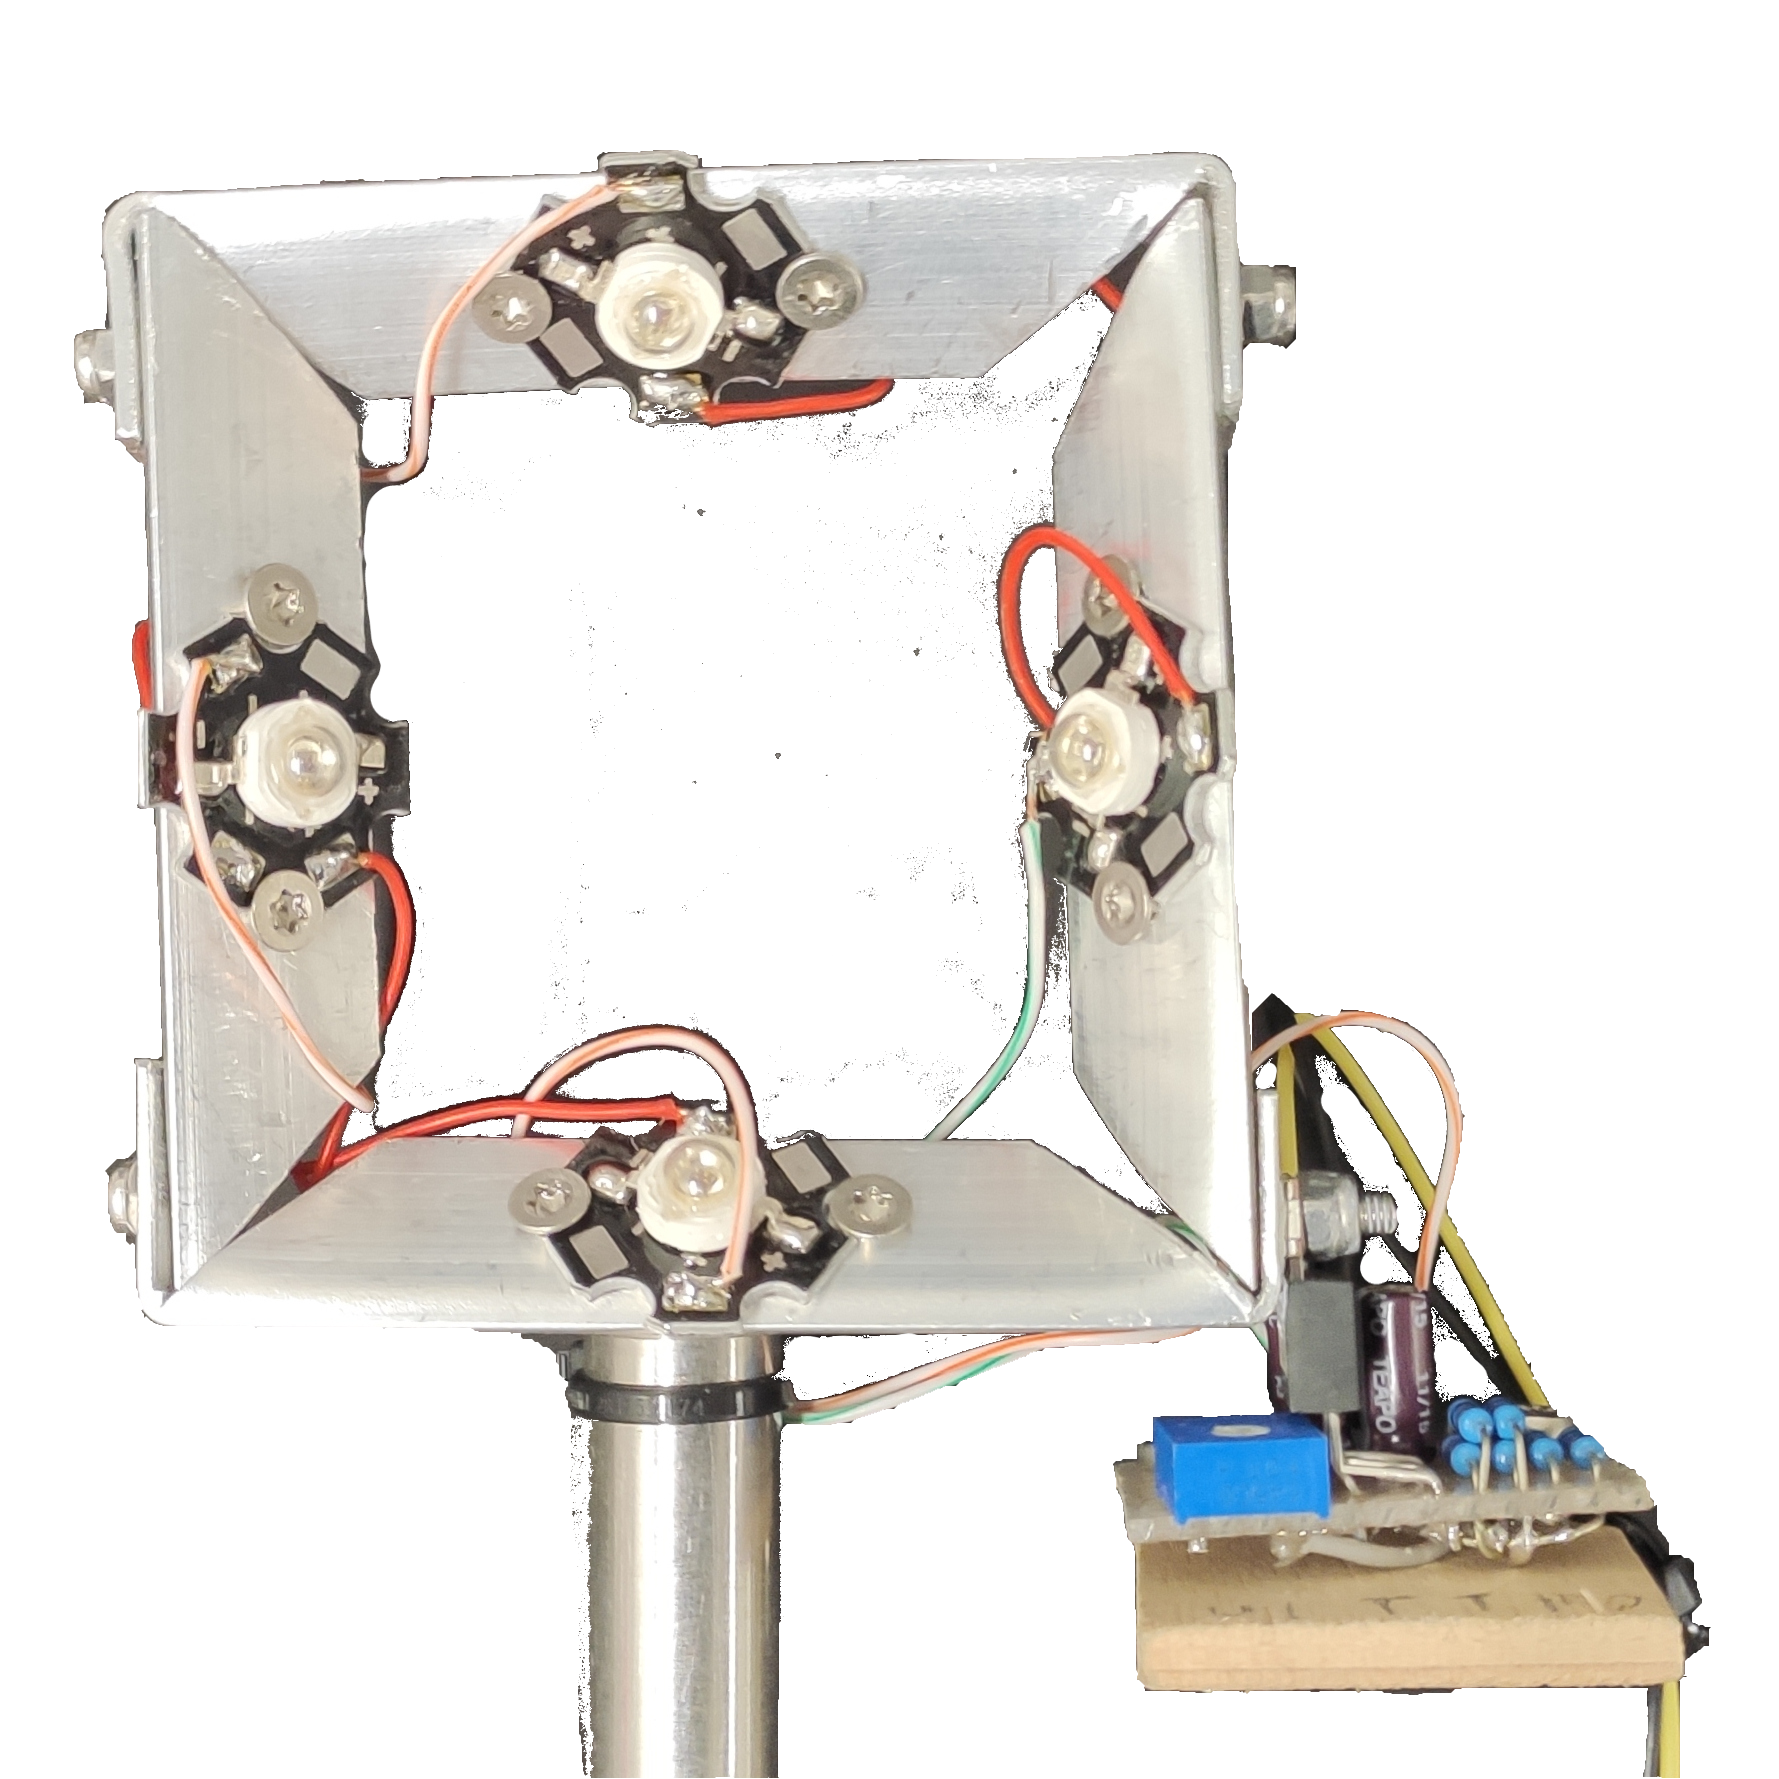
\includegraphics[width=\columnwidth]{images/TAM/RingLightFrontFree.png}
\caption{Ring light with red LEDs adjacent to pump wavelength}
\end{subfigure}
\caption{Auxilary tools for alignment, focusing and use of SHG extension setup.}
\end{figure}


The 3d printed mount can be seen in fig. \ref{fig:drop-in-Mirror-mount}.
Considerations regarding use of rubber bands or 3d printed fittings were made, however it turns out just by moving the mirror drop-in mount against a solid surface, such as one of the cage plates holding the rails, is sufficiently reproducible for the sensor resolution of the camera used. Some care should be taken to adjust the tilt angle along the cage axis, however the influence of that should be minimal considering both pump and probe are always calibrated at the same mirror setting. Additionally the beam waist diameter should not change by a noticeable amount considering the theoretical variation seen in fig. \ref{fig:beamWaistCompendium}.\\

The lighting for imaging the rear sample onto the camera via the rear lens is done using a ring light with 4 LEDs, which have a spectral intensity distribution close to the intended pump beam. The spectrum can be seen in fig. \textbf{Should I put the spectrum in addendum?}.\\
It has proven beneficial to illuminate so that a only scattered light is detected, as this \textbf{should} improve contrast. Thus the LED ring is placed behind the sample, on the side of the rear camera. As this means reduced total intensity any light not scattered by the sample or reflected from nearby surfaces needs to be blocked. For this carton is placed around the rear cage rails, blocking any light reflected from the sample mount from reaching the camera.
%The LEDs are mounted onto a square aluminium frame and are angled towards the sample to illuminate it evenly. To properly setup the focus light that not passing through the lens has to be minimized or contrast will be lost. To focus properly a small scratch is introduced to the edge of the sample, which allows better contrast for focusing as well and allows to focus closer to the center to the layer than to the top or bottom of the layer. (eh questionable, think better)

\paragraph{Use}
During use care has to be taken that there is no clipping at the drop in mirror, as this would obviously ruin the beamshape. As mentioned before if there is an OD filter directly in front of the camera for one beam fitting, there should be an OD filter there as well for the other beam, as this may cause a change in the observed beam shape.\\
For high energy SHG light absorptive OD filters have far stronger absorption than for their calibrated range, thus they may need to be swapped for a lower value. With this effect also an "amplification" of observed fundamental light from the SHG stage is introduced, which is further increased by the CMOS sensor having less quantum efficiency at these wavelengths. Thus it is important to check if the fundamental wavelength has a strong influence on the observed point spread function.\\
This can be done by introducing more glass filters, in case their absorption of the fundamental is lacking for the wavelength. The glass filters may be removed afterwards if the detector is using the prism setup, which removes the fundamental wavelength from the measurement.\\
Another option to check is to remove the fundamental filter completely and check the position of the fundamental focus spot in relation to the SHG focus spot, which will be different due to chromatic focal shift.

\subsubsection{Regular Focusing after Cage}\label{regRearFocus}
This is the option used for the regular TAM setup as described in section \ref{RegTAM}. The last mirror in front of the detector is simply removed to reveal a camera behind it. The rear cage objective is focused onto this camera using white light from an LED torch or similar lightsources in transmission. Afterwards the front objective is moved such that a satisfactory point spread function of the beam is seen from the camera sensor.\\ 
This is sufficient as the achromatic objectives allow a very similar focus for all wavelengths between 400 nm and 940 nm. The rear objective simply projects the point spread function of the beams in the plane of the sample to which it was focused to, while moving the front objective adjusts the part of the focusing beam cone, and thus the size of the slice of the beam, which interacts with the sample. This is working for both pump and probe.\\
Since the focal length of the lenses varies wildly in the UV this is not an option for the UV extension.
\subsubsection{Conversion screen for overlap adjustment}
An idea, later on abandoned for impracticality, was to use a "dummy" sample acting as a screen to then be imaged onto the camera in the rear using the lens. This method has several requirements:
\begin{itemize}
\item The screen needs to allow for diffuse imaging of the sample without disturbing the beamshape too much.
\item Any UV or near UV light needs to be converted to the visible region, where the focal length difference becomes negligible.
\end{itemize}

The requirement for diffuse imaging is simple. Any collimation or focusing action of the beam needs to be lost to actually image the sample plane, where the "dummy" is placed at. The requirement is less stringent for wavelengths close to a chosen wavelength to which the setup would be calibrated to, as the lenses would image the beam fine for that wavelength.\\

For the issue of UV conversion a few attempts with different dyes and paper were made, which showed varying success as to their luminescence.\\
Generally paper combined with orange gel marker (Stabilo No. 70/40) seemed to work best for conversion of UV to visible light.
Paper soaked with wax to increase transmittance and smooth out scattering alone did not work particularly well for conversion, unless combined with a text marker. Marker has to be applied ahead of the wax and on the other side of the paper, from where the wax will be applied. \textbf{(I am considering just throwing this all out, though having an off hand comment shouldn't be too bad) }

Using a microscope slide with gelled, specifically at room temperature evaporated, Stabilo marker (No. 70/40) turned out to have decent conversion efficiency, but lacks any diffusivity.  This could work, based on adjusting the cage setup to the pump wavelength, so it is correctly imaged. However at that time the rear focus was still set with white light instead of 653 nm pump adjacent light, which would not have allowed for this method. This also leads to problems as soon as the probe light has long enough wavelengths to simply transmit through the glass slide. It would need to be filtered and one would have to rely on conversion of those wavelengths via the marker to produce sensible output, which is a big gamble. An attempt at texturing the slide surface was not made, due to unavailability of suitable processing methods (I think I tried scratching etc, got to check notes). Another unanswered question is the emission spectrum of the marker gel. (lab notes  starting in june)\\

Another idea was to use thin film of coloured PMMA on top of a glass slide or simply a thin PMMA sheet. Fluorescence of an orange PMMA was shown, however not better than the marker. On top of that it proved insoluble in acetone making coating impossible.\\

Surprisingly the frontal focus point found with this projection method coincides well with the finally used frontal focus point. The mounts used should be within 0.2 mm of the sample surface position. The projection screens may add some extra extra offset, especially the gel on glass one would need adjustment.
Overall the attempted projection screen method did not seem viable and thus was not pursued further. A main disadvantage, apart from problems with wavelength conversion, is that in the best case the scattering applies a strong averaging to the beam point spread function, which does not allow for detection of deviations of the beam shape from a Gaussian distribution. Unless a very consistent and fine diffuse projection screen with good conversion to a specific wavelength band close to the pump is found, it is considered infeasible.



\chapter{Correction and Compensation Factors}\label{chap:CorrandComp}
Within this chapter multiple compensation and correction factors are introduced methodically, whose implementation is examined in detail in chapter \textbf{....}
\section{Overlap Correction}
%taken from what before was a chapter and still exits, currently duplicate
An important aspect of transient absorption measurements with non-tophat beamshapes is compensation of weighting effect, due to the intensity distributions of pump and probe beams. To understand this consider the linear dependence of the sample response regarding the pump power density on the sample \textbf{reference the derivation}. Because of this an area within the probe beam on the outer edge of the pump distribution is going to see a lower response than an area which overlaps the peak power density of the pump beam. This means that parts of the probe point spread function have a different sample response. Also to be accounted for is that the power density of the probe also varies like a Gaussian, thus leading to another weighting of power densities that see a certain pump power density.
This can be visualised by looking at the product of two Gaussians and how it changes when their center points $\mu$ are shifted or their $\sigma$ is changed:\\ 
\textbf{reference the calculation in the back} \ref{deriv:RadianceResponse}

\begin{figure}[!hb]
\centering
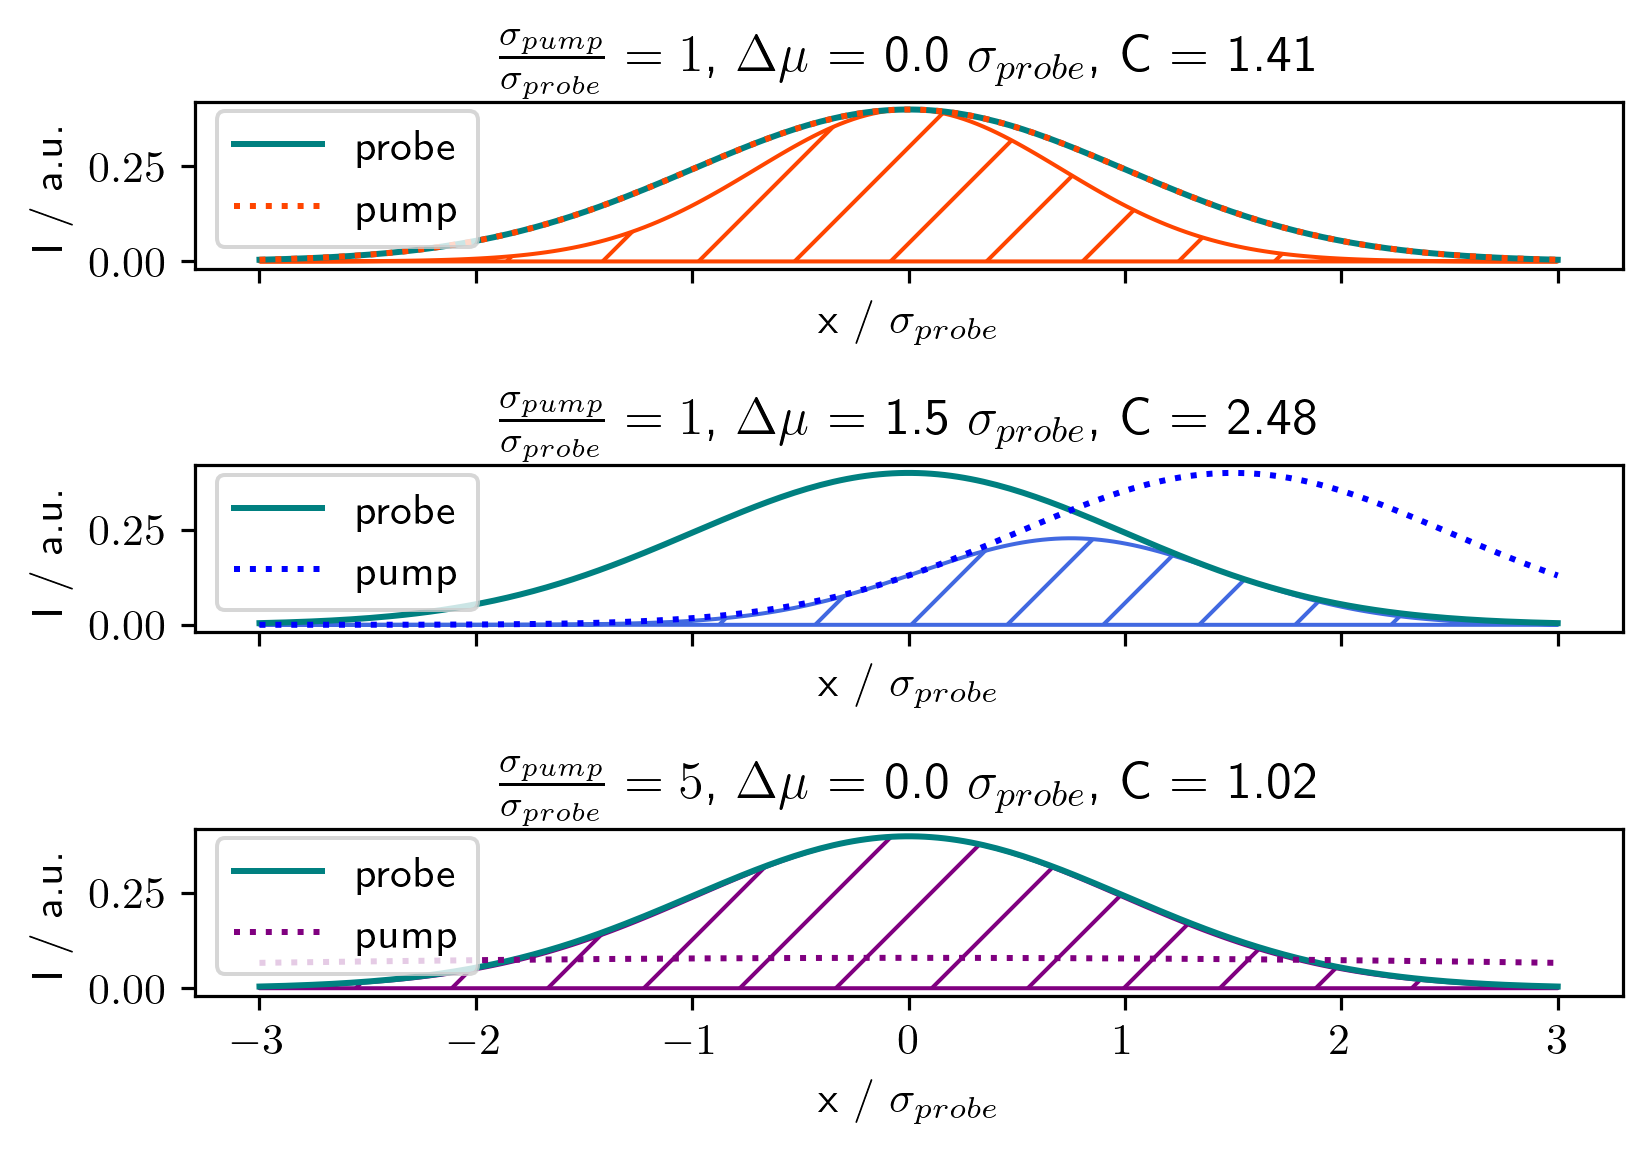
\includegraphics[scale=1]{images/OverlapVisualisationProbeSelection.png}
\caption{Selection of probe point spread function based on spatial pump-probe overlap. C is the correction factor calculated according to \textbf{insert reference when finished}. Hatched area shows the weighting of the probe happening due to linear pump power dependence of transient response.}
\end{figure}

\section{Degradation Compensation}
The samples used show a reduced response over increased exposure times to the pump and probe beams. A simple dose related model is used, where $A(t)$ is the response, $t$ is the total exposure time of the sample spot, $\tau_{1/e}$ is the degradation time constant where the response falls to 1/e and $P_{peak}$ is the maximum pump power density.
\begin{equation}
A(t) = A(t_0)\cdot e^{-\frac{(t-t_0)}{\tau_{1/e}}\cdot P_{peak}}
\end{equation}
A detailed look at data along with reasoning to why this model is used is shown in \ref{sec:degradation}.

\section{Sample variation correction}
Due to inhomogeneities of the sample the response varies over its area. This is attempted to correct for by first mapping the sample at a known GSD probe wavelength, here 680 nm were chosen, and then is measured in a grid-like manner. Related measurements are then multiplied with a relative factor, to normalise their response. This should be a valid approach for pump radiances below threshold for  non-linear processes.

\section{Background subtraction}
All measurements carry a constant background offsetting the measurement ahead of pump and probe temporal overlap, thus probe passing through the sample ahead of pump. This mainly is due to stray light of the pump beam reaching the sample. \textbf{are there other detector influences?} A correction is made by shifting the $\mathrm{\frac{I_{pump-probe}}{I_{probe\, only}}}$ in such a way, that it is 1 ahead of the temporal overlap point. \\
However sometimes a linear component, for example from minor pump movement due to imperfections of the stage along its travel, is observed. If the linear component is small enough it may similarly to a static offset be corrected by a linear fit of the ratio $\mathrm{\frac{I_{pump-probe}}{I_{probe\, only}}}$. Once the component is too large a measurement has to be considered faulty. Depending on how large the linear component is decay constants may not be viable, however the immediate response after temporal overlap may be considered correct after subtracting the linear component.\\

Theoretically the correct way of applying a background subtraction, under assumption that it indeed only is stray pump light, would be to only subtract the background from $\mathrm{I_{pump-probe}}$. This is not possible however, due to temporal variations in probe intensity, which do cancel for the ratio $\mathrm{\frac{I_{pump-probe}}{I_{probe\, only}}}$.



\chapter{Overlap Correction}\label{chp:OverlapCorrection}
%An important aspect of transient absorption measurements with non-tophat beamshapes is compensation of weighting effect, due to the intensity distributions of pump and probe beams. To understand this consider the linear dependence of the sample response regarding the pump power density on the sample \textbf{reference the derivation}. Because of this an area within the probe beam on the outer edge of the pump distribution is going to see a lower response than an area which overlaps the peak power density of the pump beam. This means that parts of the probe point spread function have a different sample response. Also to be accounted for in that the power density of the probe also varies like a Gaussian, thus leading to another weighting of power densities that see a certain pump power density.\\
%This can be visualised by looking at the product of two Gaussians and how it changes when their center points are shifted or their $\sigma$ is changed:\\ \textbf{do a plot}
\section{Overlap Compensation}
Opposed to the old setup, where the achromatic objectives guaranteed relatively consistent overlap of pump and probe, the UV setup has the need to correct the variation between the single measurements, since the diffraction of the dispersive elements in the probe path varies strongly in the UV range and any compensation via the telescope will be imperfect.\newline
Relevant for this are the beam size of the probe as well as the overlap of the pump and the probe beam in the sample. Variations in those parameters are induced by change of the beamshape due to SHG generation, imperfect alignment of the SHG telescope and correction of the chromatic aberration for different wavelength settings of the probe.\newline

\subsection{Beam Characterisation}
The python class ArtFit has some options to check for the validity of the data used. \textit{Data is saved in a raw format, however it is cut and thus an offset for the ROI has to be accounted for.} The beam shape is saved as a raw file corresponding to the ROI set in LiveFit. As the raw data is cut to the ROI an offset has to be accounted for, to remove the background covering the entire sensor correctly.

ArtFit may parse 3 different input types:
\begin{enumerate}
\item Quick plotting of raw data:\\
With a path to a raw data file and an optional bool value, which is used to tell the program to use the standard size of 1280x720 instead of a square pixel array size deduced from total number of entries. Plots the beam intensity profile without any processing.
\item Single beam profile with background subtraction: \\
Loads a JSON with a dictionary for background subtraction, the path for the beam profile to be loaded and a width for fitting.
\item Two beam profiles with background subtraction: \\
ROI offset has to be identical and is again defined by a JSON file with background location.
\end{enumerate}

To get meaningful data for correction of data the pump power has to be set using setPumpPower() and the scale can optionally be overwritten from the background file with setScale(). Fitting is done by calling plainFit(id), where id = 1 for probe (first filepath handed over) and id = 2 for pump (second filepath).

Some options to show the images as well as the fits are:
\begin{itemize}
\item plotComp()\\
Shows an intensity contour plot of both beams on top of each other. If only one beam file is loaded only one is shown. Also shows the fitted intensity slices on top of each other for both pixel array axis. Returns an overlap value corresponding to what is given by the liveFitting program described in section \ref{Sec:LiveFitting}.
\item plotGauss()\\
Plots the intensity profile of the beams, if both are given, separately with an overlayed contour plot of the fits, to allow to ascertain the validity of the fit. Needs to have already fitted data with plainFit() to show the Gaussian distribution. Fitted data may be printed to console by setting printData = True for the options. The intensity profile is shown by default without background subtraction and can be shown with subtracted background by handing over a boolean. The fits are always done with subtracted background, the profile just is not shown background subtracted by default.
\end{itemize}
\subsection{Correction Factor}\label{sec:CorrFactor}
The correction factor aims to equilibrate the transient absorbance of the given pump-probe overlap to one where the pump is constant in radiance over the entire probe area or in a physical description is infinitely larger than the probe beam. 
Thus for very high $\mathrm{\frac{\sigma_{Pump}}{\sigma_{Probe}} \rightarrow \infty}$ the correction factor tends to 1, which is the smallest value.\\
%The factor is calculated from the Gaussian intensity distributions as seen in eq. \ref{CorrFactorGaussians}, of which the derivation is shown in section \ref{GaussiansDerivation} or in Bromiley\cite{Bromiley2014}, which was used to check correctness. The enumerator is the integral over essentially the probe intensity with the constant factor of the maximum pump intensity 
The idea of the factor is a normalisation of the overlap of the beams to an ideal state. This ideal state corresponds to an equal pump intensity over the entire probe beam, that would allow the entire probe to experience the same change in absorption. Thus the correction factor C is chosen as the integral over the product of the ideal pump, an infinite plateau, with the Gaussian probe. The denominator on the other hand is the integral over actual product of the Gaussian fits of pump and probe beam.
\begin{equation}\label{eq:CorrFactorGaussians}
C = \dfrac{\int I_{pump}^*\cdot I_{probe}(x) \;dx}{\int I_{pump}(x)\cdot I_{probe}(x) \; dx} = \dfrac{c^*\cdot \int I_{probe} dx}{S_{12}} = \dfrac{c^*}{S_{12}}
\end{equation}
The ideal plateau pump is chosen to be the maximum of the actual pump normal distribution, to decouple correction factor from the pump width. \textbf{Rethink and justify the reasoning physically:  } The ideal constant pump power density is set to be the same as the maximum of the real beam. Reasoning for that is that some referencing to the power density of the real pump is needed, since otherwise the correction is no longer independent of the pump power. Since the actual intensities are not considered, but only the shape of the Gaussians the same intensity defining variable is used as for the actual Gaussian:
\begin{equation*}
I_{pump}^* = c^* = max(I_{pump}(x)) = \frac{1}{\sqrt{2\cdot\pi}\cdot\sigma_{pump}}
\end{equation*}

$\mathrm{S_{12}}$ is defined as can be seen in eq. \ref{eq:S12CorrectionFactor} and serves as the extra normalisation factor for rewriting the product of the two Gaussians into a single Gaussian. The derivation of the single Gaussian can be seen in \ref{GaussiansDerivation} and has been cross-checked with Bromiley.\cite{Bromiley2014}

\begin{equation}\label{eq:S12CorrectionFactor}
S_{12} = \dfrac{1}{\sqrt{2\pi\left(\sigma_1^2+\sigma_2^2\right)}}\cdot exp\left(-\dfrac{\left(\mu_1 - \mu_2\right)^2}{2\cdot \left(\sigma_1^2+\sigma_2^2\right)}\right)
\end{equation}

This leaves the full correction factor C to be:
\begin{equation}\label{eq:fullCorrectionFactor}
C = \sqrt{\frac{\sigma_1^2+\sigma_2^2}{\sigma_1^2}}\cdot exp \left(\frac{\left(\mu_1-\mu_2\right)^2}{2\cdot \left(\sigma_1^2+\sigma_2^2\right)}\right)
\end{equation}

A few illustrations of the behaviour of the correction factor are shown in fig.

Furthermore to have all relative $\mathrm{\Delta OD}$ values be directly comparable, the correction factor is divided by the peak radiance value.

\begin{table}[h]
\caption{Illustrative one dimensional correction values for fitted Gaussians}
\centering
\begin{tabular}{c|rrrrrr}\toprule
$\Delta \mu$ / $\sigma$                     & 0          & 0             & 0              & 0             & 1              & $2\cdot\sqrt{2 ln(2)}$ \\
$\dfrac{\sigma_{pump}}{\sigma_{probe}}$ / 1 & 1          & 3             & 2              & 1/2           & 1              & 1                      \\
Correction Factor                           & $\sqrt{2}$ & $\approx1.05$ & $\approx 1.12$ & $\approx 2.24$ & $\approx 1.82$ & $\approx 5.66$ \\ \bottomrule       
\end{tabular}
\end{table}


To ascertain how well this works a numeric variant of the correction factor is considered based on the same principle as eq. \ref{eq:CorrFactorGaussians}:
\begin{equation*}
C_{numeric} = \sum_{i=0}^{N_x}\sum_{k=0}^{N_y}\frac{\mathrm{max}\left(I_{pump}\right)\cdot I_{probe}(x_i,y_k)}{I_{pump}(x_i,y_k)\cdot I_{probe}(x_i,y_k)}
\end{equation*}
where $\mathrm{x_i/y_k}$ are discrete points, which may be associated with single pixels of the camera, of which there are $\mathrm{N_x}$ for $\mathrm{x_i}$ and $\mathrm{N_y}$ for $\mathrm{y_k}$. $\mathrm{max\left(I_{pump})\right)}$ once again is the maximum value of $\mathrm{I_{pump}}$ over all $\mathrm{x_i, y_k}$. For this definition $\mathrm{I_{pump}/I_{probe}}$ may be of arbitrary noisy form, which is what will be tested in the following.

Comparing the numeric approach with the analytic fitting approach is done by generating a hypothetical pump and probe Gaussian pair, for which the correction factors are calculated. The analytic value is generated directly from the generating parameters for the numeric discrete map. For $\mathrm{I_{pump} = const}$ the correction factor trivially goes to one as per definition. Since the discrete values strongly depend on the number of bins an approach is chosen, where a density of discrete points per $\mathrm{\sigma}$ of the generating Gaussian distribution is shown. To visualize this the correction factor of a "pump" and "probe" combination, where $\mathrm{\sigma}$ and $\mathrm{\mu}$ are identical for both distributions, is show over a number of bin sizes is shown in fig. \ref{fig:NumericalCorrectionSNR}. The bin size is chosen so that always a multiple of two discrete values per axis is binned together and the bins are kept square in size. The influence of a noise component, randomly distributed for a specific signal to noise ratio, is also shown.

\begin{figure}[h]
\centering
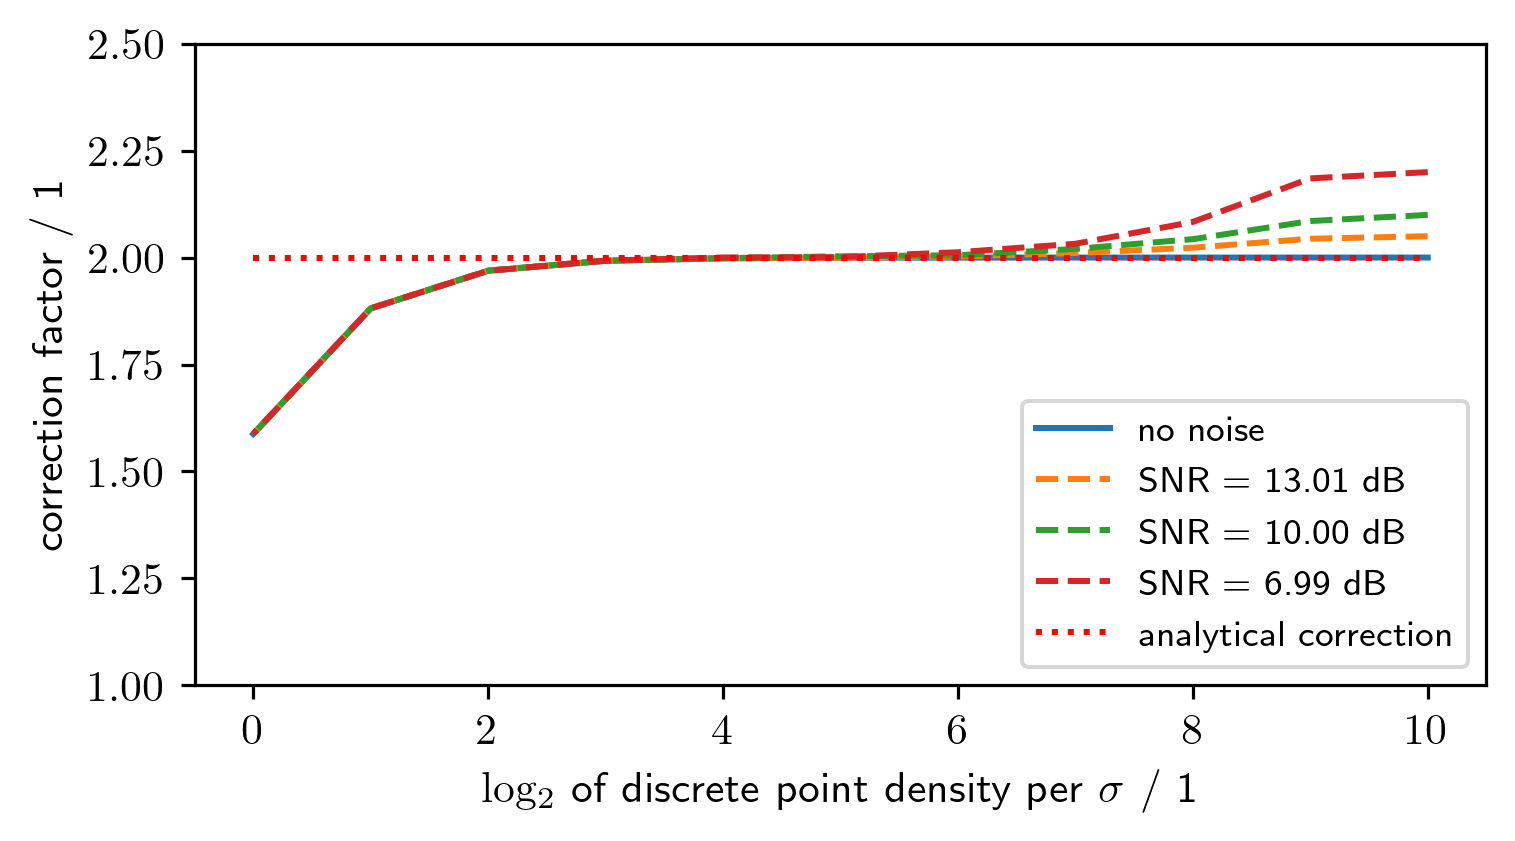
\includegraphics[scale = 1]{images/NumericalCorrectionSNR.png}
\caption{Comparison of numerical and analytic correction factors for radial-symmetric Gaussian distributions of identical parameters. \\$\frac{\sigma_{pump}}{\sigma_{probe}}=1$,$\Delta\mu = 0$\\For the case of the SNR graphs a random noise was added individually to both distributions.\label{fig:NumericalCorrectionSNR}}
\end{figure}

To check for possible effects regarding offsetting of the distributions from the pixel grid and breaking the symmetry from above the Gaussian distributions are now shifted by 1 $\mathrm{\sigma}$ in both x and y direction from each other in fig. \ref{fig:NumericalCorrectionShift}. Furthermore both distributions together are shifted by an offset from the pixel grid in x direction. Doing this incremental shift in both x and y direction only leads to a small change for large binning sizes. 

\begin{figure}[h]
\centering
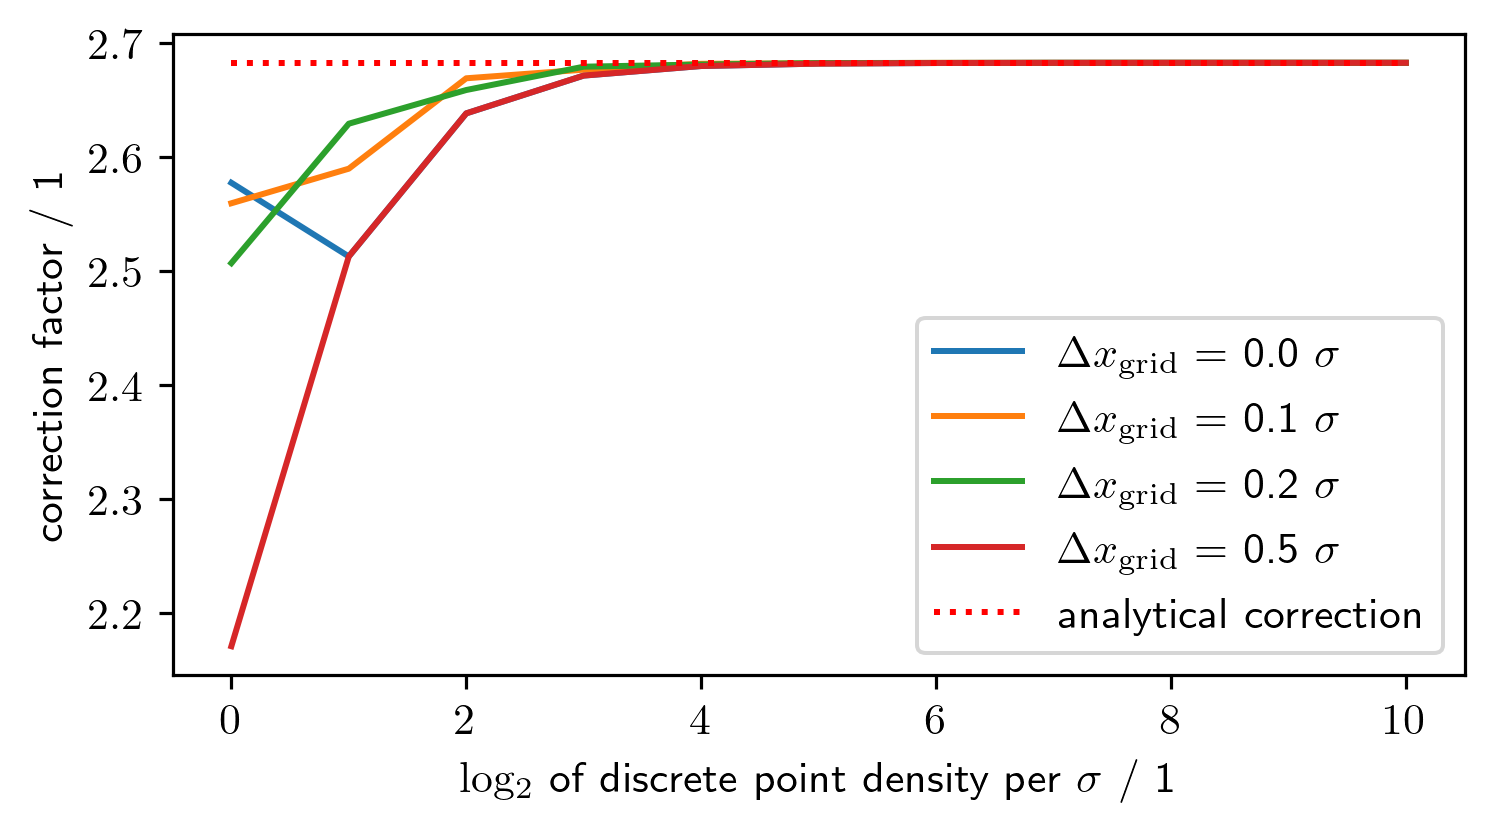
\includegraphics[width=0.9\linewidth]{images/NumericalCorrectionShiftedBeams.png}
\caption{Comparison of analytic  and numeric overlap correction factor with varying shift regarding simulated pixel lattice in x direction
\\$\frac{\sigma_{x-pump}}{\sigma_{x-probe}}=0.8;\frac{\sigma_{x-pump}}{\sigma_{x-probe}}=2.0;\Delta\mu = \sqrt{2}$\label{fig:NumericalCorrectionShift}}
\end{figure}
\textbf{NOTE SOMEWHERE: the actual size of the point spread function on the sensor is at about 2-4 points per sig -> not sensible without fitting}

\subsection{Artray-LiveFitting}\label{Sec:LiveFitting}
As the Artray $\mathrm{ARTCAM-092UV-WOM}$ could not be interfaced with matlab using the webcam library a C\# program was created based on the manufacturers example program.
Issues with our system are that for our specific camera or system setup a periodic variation of low intensity signal is reported by the C\# based program, while this periodic variation is missing in the official software. Attempts were made to troubleshoot this in correspondence with the manufacturer, who were very forthcoming in the matter, but it could not be solved so far. To overcome this problem a simple background subtraction has been devised as sufficient, as the variation seems to be constant over time. The background has been recorded with the lens cap on at an exposure of 15 ms, which was chosen after comparing the subtracted quality output of 0.3 ms, 15 ms and 100 ms. 
\newline
For all measurements included here version 1.2 was used. The  ALGLIB software package is used\footnote{ALGLIB for C\# 3.19.0 licensed as per GPL 3} for fitting a Gaussian to the beamshape. Scottplot 4\footnote{Copyright 2018 Scott Harden, MIT License} is used to display the fitted data.\\
\subsubsection{Fitting principle}
In version 1.2 the relevant fitting parameters are returned as a numeric overlap integral based on the Gaussian beamshapes. In this version it is still calculated numerically from the fits, however it can be rebased into an analytical form as per eq. \ref{eq:GaussianProduct} which describes the product of two Gaussians.
\begin{equation}
\mathrm{overlap} = \int \sqrt{f_1(x)*f_2(x)}dx =  \sqrt{\frac{2 \sigma_1^2\sigma_2^2}{\sigma_1^2+\sigma_2^2}}\cdot exp\left(-\frac{\left(\mu_1-\mu_2\right)^2}{4\cdot \left(\sigma_1^2 + \sigma_2^2\right)}\right)\label{eq:GaussianProdcut}
\end{equation}
This is calculated separately for both axis of the pixel array and then multiplied for a final value. 
This is not directly related to correction factor calculated within the python program to make everything comparable, but is more of a measure of how similar the beams are, which is why only the normal distributions are used without an intensity modifier, thus both beams are weighted identically. \\
This is reasonable as the best results for the correction factor are achieved when pump and probe beams are similar in size. This overlap integral returns a maximum value of 1 when the beams are identical and falls off quickly if the intensity maxima are shifted and slowly if the FWHM of the beams is different.\\
\subsubsection{Operation}
Before startup all needed DLL files need to be in the same folder as the executable.\footnote{alglib.net.dll, ArtCamSdk\_092UV\_WOM.dll, ScottPlot.dll, "ScottPlotWinForms.dll", Python.Runtime.dll,...} need to be in the same folder as the executable. Additionally .NET Framework 3.5 is required. Upon startup the program should automatically connect to the camera. \\
The main forms shown upon startup are the camera control form in fig. \ref{fig:ArtrayMain} and the fitting form in fig. \ref{fig:ArtrayFitting}.

\begin{figure}[hbtp]
\centering
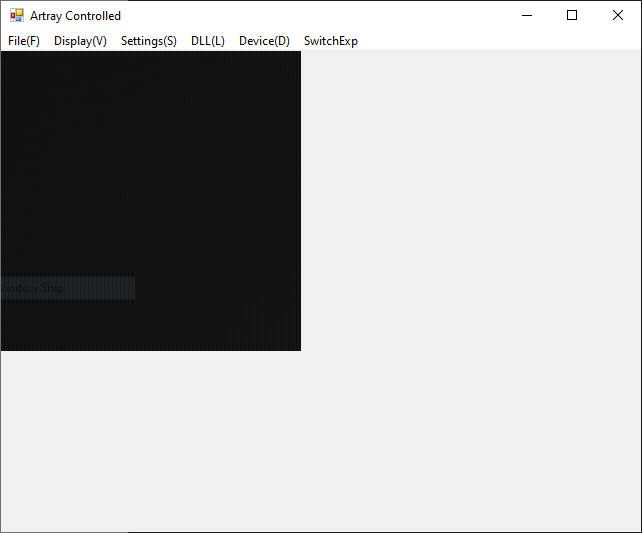
\includegraphics[width = 0.6\linewidth]{images/ArtrayExamplePics/ArtrayControlledMain.PNG}
\caption{Artray Controlled window\label{fig:ArtrayMain}}
\end{figure}

\begin{figure}[hbtp]
\centering
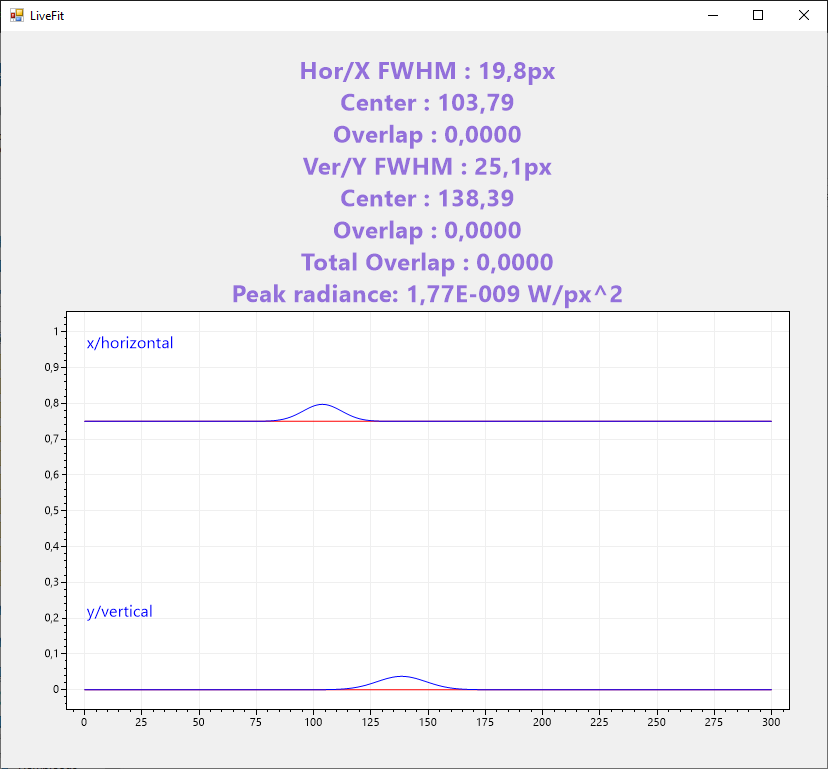
\includegraphics[width = 0.6\linewidth]{images/ArtrayExamplePics/FittingForm.PNG}
\caption{Fitting form artray\\Scottplot 4 is used to generate the output for this figure.\label{fig:ArtrayFitting}}
\end{figure}


To get an image there are several options in the "Display" drop down menu.
\begin{itemize}
\item Preview: starts a livestream within the "Artray Controlled" window.
\item Snapshot: takes an image and statically shows it. If possible a fit will be shown in the "LiveFit" window.
\item Callback: starts a livestream with periodic fitting. Preview should be preferred if no fitting is needed or possible for performance reasons.
\end{itemize}

To adjust the image parameters or camera settings use the "Settings" drop down menu.
\begin{itemize}
\item Camera settings: opens a menu to set the image format including size and ROI as well as Color format, which is to be set to "Color 48*bit" for reasons that are explained in raw data output. The effective ROI should be set to 300 pixels vertically and horizontally. The ROI should stay square and not rectangular, as there is a bug preventing correct data manipulation at this moment. An example of the settings can be seen in fig. 
\item Filter settings: include software settings for brightness, contrast, saturation etc. Influence of Bayer Mode on the monochromatic sensor is unknown, as it does not show an obvious difference in output. Keep the saturation at -255.
\item Analog settings: consist of gain and exposure. Also has the option to mirror image vertically and horizontally, which should not be done after calibration. There is no way of telling from raw output data at which setting a snapshot was taken.
\item Misc: is where custom settings for output parameters as well as exposure can be set. Assigning a "µm per px" value and adjusting the power correctly allows a readout directly corrected peak radiance and other fit parameters such as the FWHM.\\The three exposure values can be quickly jumped to from a drop down menu in the main window and are supposed to help streamline the measurement process. The menu can be seen in fig. \ref{LiveFitting:MiscMenu}.
\end{itemize}

\begin{figure}[hbtp]
\centering
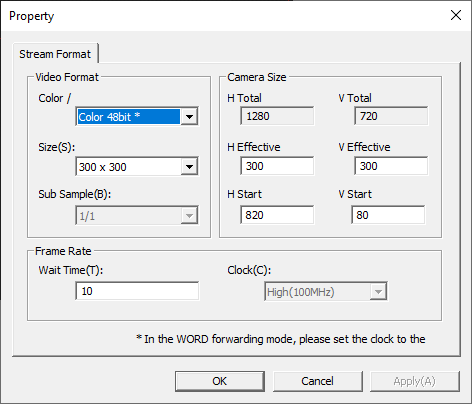
\includegraphics[width = 0.6\linewidth]{images/ArtrayExamplePics/StreamProperties.PNG}
\caption{Menu for camera settings given by Artray\\ Example settings to get good data output within a square ROI.}
\end{figure}

\begin{figure}[hbtp]
\centering
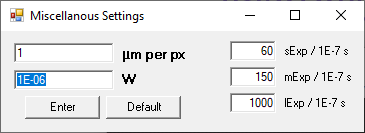
\includegraphics[scale=1]{images/ArtrayExamplePics/DefaultMiscSettings.PNG}
\caption{Miscellaneous menu for setting quick change exposure values and additional constants to correct fitting output.\\
Default value of µm per px means that the fitting form only shows the FWHM and related values in units of pixels.\\
The exposure values are in 0.1 µs steps, as this is what the camera allows. Only integer input is supported.\label{LiveFitting:MiscMenu}}
\end{figure}



As mentioned quick swap exposure settings can be set. They are accessed from the drop down menu "SwitchExp". Upon switching exposure a snapshot is taken, this interrupts all other image acquisition types, and a maximum pixel intensity is reported in a pop up window, to show if the dynamic range of the camera is being used well. If that is not the case the fitting window either turns blue if the exposure is too low (30\% of max) or turns red if it is too high (95\% of max). Setting exposure can in cases be slower than readout of the snapshot, thus reporting a value ahead of setting the new exposure value. If that is the case just set exposure again if one wishes to get the maximum pixel intensity value.\\

The file drop down consists of features for saving, opening and comparing data:
\begin{itemize}
\item Save: saves a raw txt file of the last captured image. In case of a livestream this is the last shown image. For snapshot it saves the currently shown snapshot.
\item End: Ends the program
\item Reference: sends a reference image, behaviour is like with save regarding livestreams, to the "LiveFit" window. There a fit of the reference is shown as a red graph, which when not set is flat.
\item Open: works like reference, however it opens the reference snapshot from a raw txt file of choice via file dialogue.
\item Background: sets a background to subtract from the images for live fitting. Setting background does not alter the behaviour of Save. Saved files are still plain raw unaltered data from the sensor. The background file location is automatically loaded when starting a session and is saved in the windows registry. under $\mathrm{"Computer \backslash HKEY\_CURRENT\_USER \backslash SOFTWARE \backslash LiveFit"}$as BACKGROUND\_FILE. The LiveFit subkey needs to be created manually, possible with regedit\textbf{AUTOMATE}, ahead of use. The BACKGROUND\_FILE subkey is automatically added or handled.
\end{itemize}


\chapter{SQIB in PMMA}\label{chpt:results}
In this chapter the main results, a wavelength scan of extended wavelengths, is presented and details of the sample is discussed. The motivation was to find excited states of higher energy than previously reported to use for modelling purposes. Other than an extension of the falloff of the ESA peaks and a qualitative reproduction of the results of Zheng\cite{Zheng2020} however no further peaks could be defined.

\section{1wt\% SQIB in PMMA matrix}
The sample is 1wt\% SQIB in a PMMA solid solution. The sample is not annealed and shows fluorescence if illuminated by white light, implying the influence of neighbouring molecules is not strong enough to quench the fluorescence at this concentration. \\

Opposed to liquid solutions like $\mathrm{CHCL_3}$ there is no quick solvent reorganisation for n-butyl terminated squaraine molecules within PMMA. It is assumed that the relatively fixed structure of the squaraine hinders structural rearrangement within the rigid PMMA matrix. With similar bulkiness of the isobutyl sidechains used here there also should be no fast solvent reorganisation. \cite{Zheng2020}

An average nearest neighbour distance for this concentration may be taken as \SI{2.36}{\nano\meter} according to Zheng et al. \cite{Zheng2020}, who based the calculation on poisson statistics\cite{Krider2003}. The actual spread of nearest neighbour distances is a large distribution. Thus there is an expectation of some quenching of effects such as fluorescence as well as decay times of excited states. However all effects are still observed due to the distribution of nearest neighbour distances as well as random rotation of nearest neighbours to each other, leading to inefficient charge transport or quenching.\cite{Zheng2020} \\
Collective effects like Davydov splitting, which are dependent on a relative orientation of transition dipole moments of subunits, are negligible for samples that are not annealed at this kind of concentration and are not observed.\\

\begin{figure}[!htp]
\centering
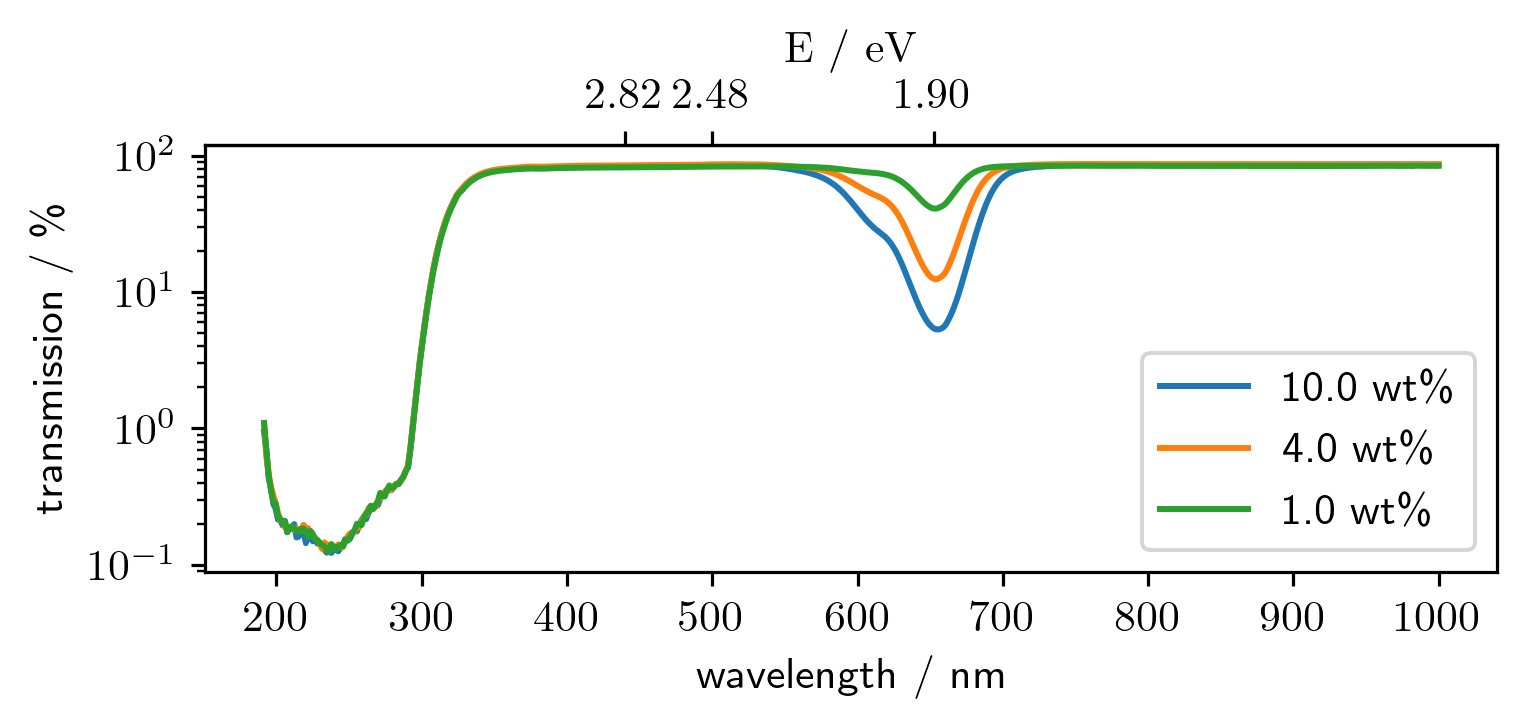
\includegraphics[scale = 1]{images/SQIB_VarPercentInPMMA_transmission.png}
\caption{Continuous wave transmission spectrum of the varying percentages of SQIB in PMMA samples provided by Manuela Schiek\label{fig:VarpercentCWspectrum} \textbf{ASK HOW TO REFERENCE THIS} Reference sample with PMMA has a film thickness of roughly \SI{650}{\nano\meter}}
\end{figure}

As shown in the spectrum in fig. \ref{fig:VarpercentCWspectrum} the main CW absorption feature of isolated SQIB itself is at 653 nm. Increasing the concentration and thus introducing collective effects a widening of the absorption feature towards 600 nm may be observed. Due to the absorption of glass and the PMMA matrix itself taking over at below 300 nm no measurements below 300 nm were made.\\

\section{Wavelength dependence of 1\% SQIB in PMMA}


Even though the sample is intended to be relatively homogeneous, there are variations in sample response over the area surveyed. For the wavelength scans shown in context of the SHG setup sample spots without strong variations in the vicinity were preferred, however this method has limited resolution and limited area due to being very time intensive. An attempt to linearly compensate the difference in response has been made for some measurements and will be explicitly stated when applied. \textbf{currently everywhere, should I show something without?} Since exposure of the single spots is rather short no discernible sample degradation is expected from these mapping operations. The map used for correction of the shown wavelength scans may be seen in fig. \ref{fig:TA_image_sample}. Pump power before and after measurement are identical, however probe power varied over time.\\
Also applied is the overlap correction factor with a fitting width using a 3 px average centered on a peak fit. Degradation compensation is applied as described in sec. \ref{sec:degradation} using the same $\tau_{1/e} = \SI{14100}{\second}$ compensated for the peak pump power used in the measurement.
Measurements are done in parallel pump and probe polarization.

\begin{figure}[hbt]
\centering
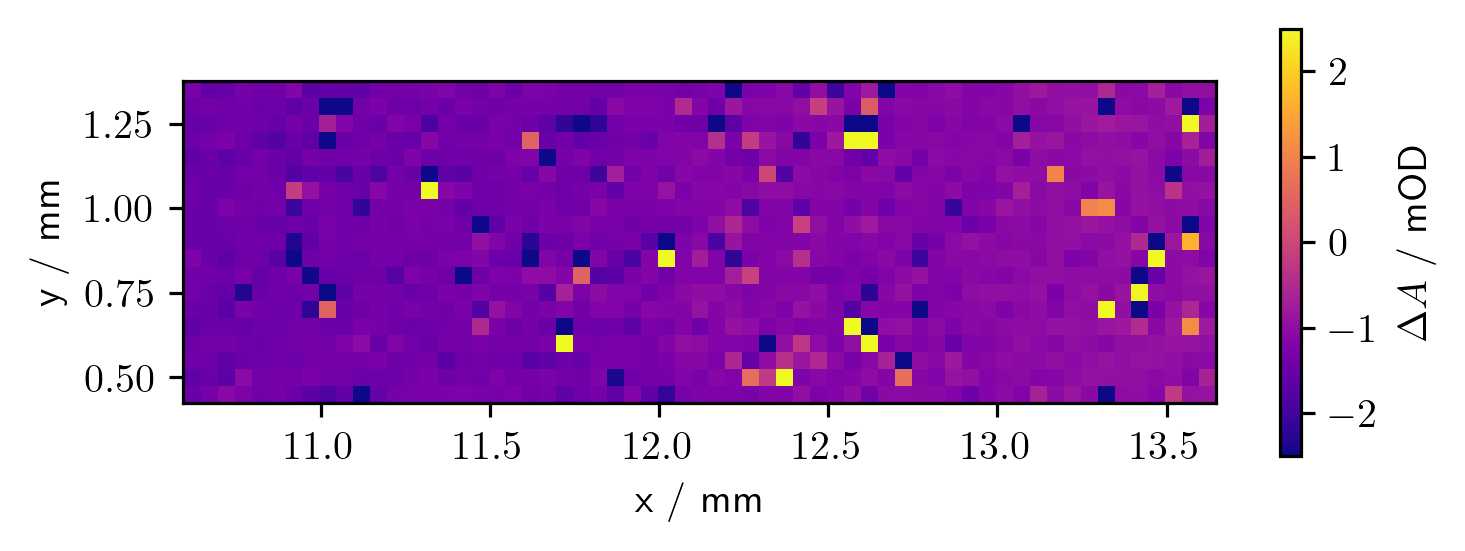
\includegraphics[scale=1]{images/1percentSQIBinPMMA_Sample653-680Image.png}
\caption{Transient absorption image of 1wt\% SQIB in PMMA sample from image\_0245 with subtracted background image\_0244 at a probe spot size of approximately \SIrange{36}{45}{\micro\meter} FWHM.\\ Extreme deviations from standard power are likely to be imperfections in or on the sample and have to be avoided for measurements.\\ Pump peak radiance at \SI{653}{\nano\meter} approximately \SI{85e-3}{\radExp}, probe peak radiance at \SI{680}{\nano\meter} approximately \SIrange{7.5e-3}{12.5e-3}{\radExp}\label{fig:TA_image_sample}}
\end{figure}

The correction for variation of the sample response at different measurement points is accounted for as as a factor normalised by the mean sample response, of the used points of the probe wavelength scan, for a pump 653 nm probe 680 nm. Uncertainty estimation is unavailable due lacking resolution of the map.\\
The UV extended transient behaviour of the sample is shown in fig. \ref{fig:SQIB_PMMAwavelengthscan}, where fitted delay points are shown to see the immediate transient behaviour. They are fitted using a nonlinear curve\_fit from scipy.optimize to fit eq. \ref{eq:transientDecay}. The number of exponential components may be automatically determined by fitting, however within this thesis they are set by hand. An example for a fitted delay scan is seen in fig. \ref{fig:delayFitExample}.
\begin{equation}\label{eq:transientDecay}
f(t) = \left[\sum_{n=0}^{n_{max}} A_n\cdot exp \left(\frac{-(t-t_0)}{\tau_n}\right)\right]\cdot \int_{-\infty}^t exp\left(-\frac{(t-t_0)^2}{2\sigma^2}\right)
\end{equation}

\begin{figure}[hbtp]
\centering
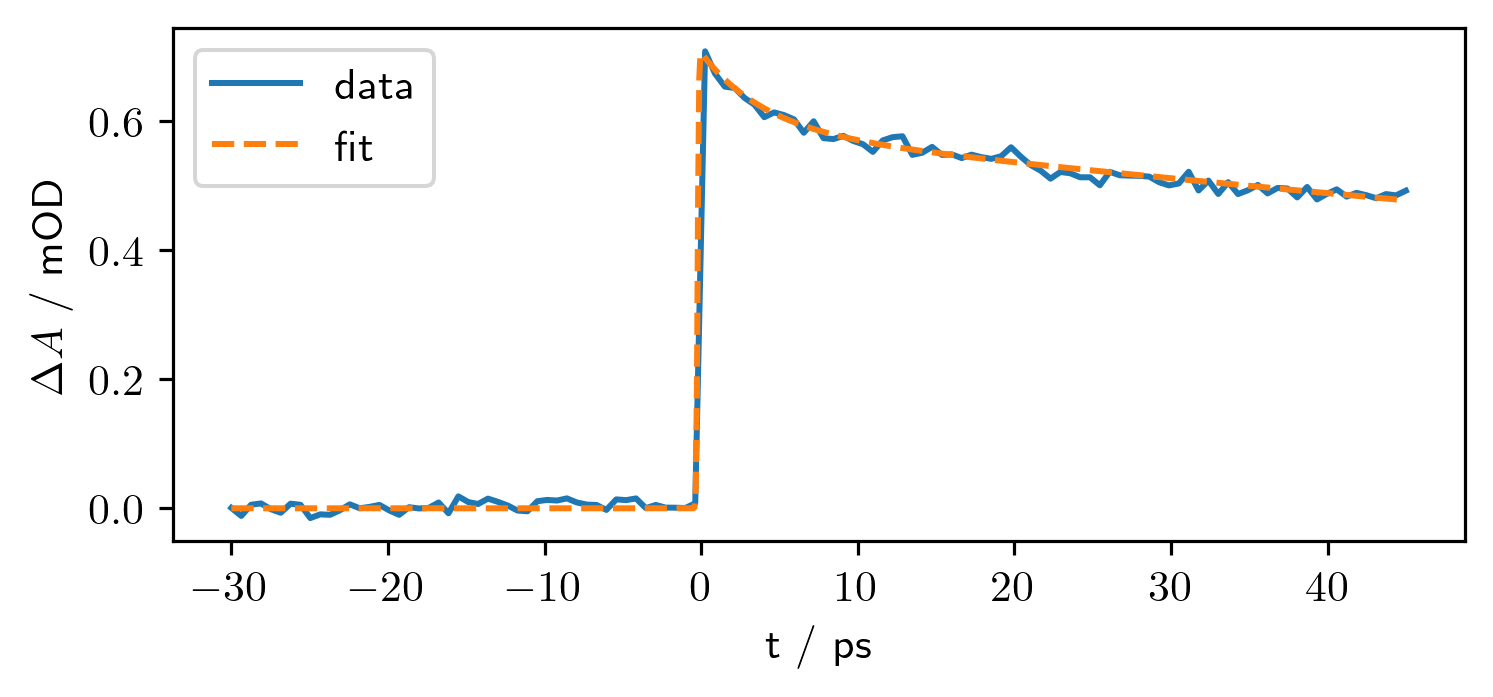
\includegraphics[scale=1]{images/ExemplaryDelayScanFit_Pump653Probe493.png}
\caption{Exemplary fit for degradation corrected average of delay scan for a pump \SI{653}{\nano\meter} probe \SI{493}{\nano\meter} combination for measurements TA\_fourier\_ 6767-6769.\\Fit parameters: $\tau_1 = \SI{4000}{\femto\second}, A_1 = \SI{0.125}{mOD}, \tau_2 = \SI{216800}{\femto\second}, A_2 = \SI{0.588}{mOD}$; Degradation compensation $\tau_{1/e} = \SI{14100}{\second}, \mathrm{P}_{\frac{measurement}{reference}} = 0.96$ \label{fig:delayFitExample}}
\end{figure}


The data is corrected for the mentioned map irregularities, degradation of the sample over measurement time and overlap of pump and probe beams. The concepts for these corrections are found in chap. \ref{chap:CorrandComp} should be, that the fits generally work well visually or regarding residuals, however uncertainties from the fits are not applicable, as the sample response decays far too slowly to realise good decay constants with available delay lengths of the setup. Thus the fits are applied such, that they replicate the data as well as possible. Choice of a single or bi-exponential decay is made for optimising the residuals, especially near the important temporal overlap edge. The power densities used in the wavelength scan are shown in tab. \ref{tab:powersWavScan} and wavelength scans shown here are normalised by their power densities, assuming the linearity of the response to the pump peak radiance.

\begin{table}[htb]
\caption{Pump peak power densities used for wavelength scan\\ At \SI{0.325}{\radiance} linearity of measurements to pump power density may already deviate, however it may still be used to check for signal response.\label{tab:powersWavScan}\textbf{is mixing bad? I am not sure on this}}
\centering
\begin{tabular}{l|ccccc}
wavelength range / nm           & \SIrange{680}{400}{}   & \SIrange{390}{380}{}   & 370  & \SIrange{360}{350}{}& \SIrange{330}{310}{} \\ \midrule
peak power density / \SI{e-3}{\radExp}& \SIrange{75}{85}{} & \SIrange{90}{120}{} & \SI{150}{} & \SI{325}{}  & \SIrange{190}{195}{} 
\end{tabular}
\end{table}



\begin{figure}[hbt]
\centering
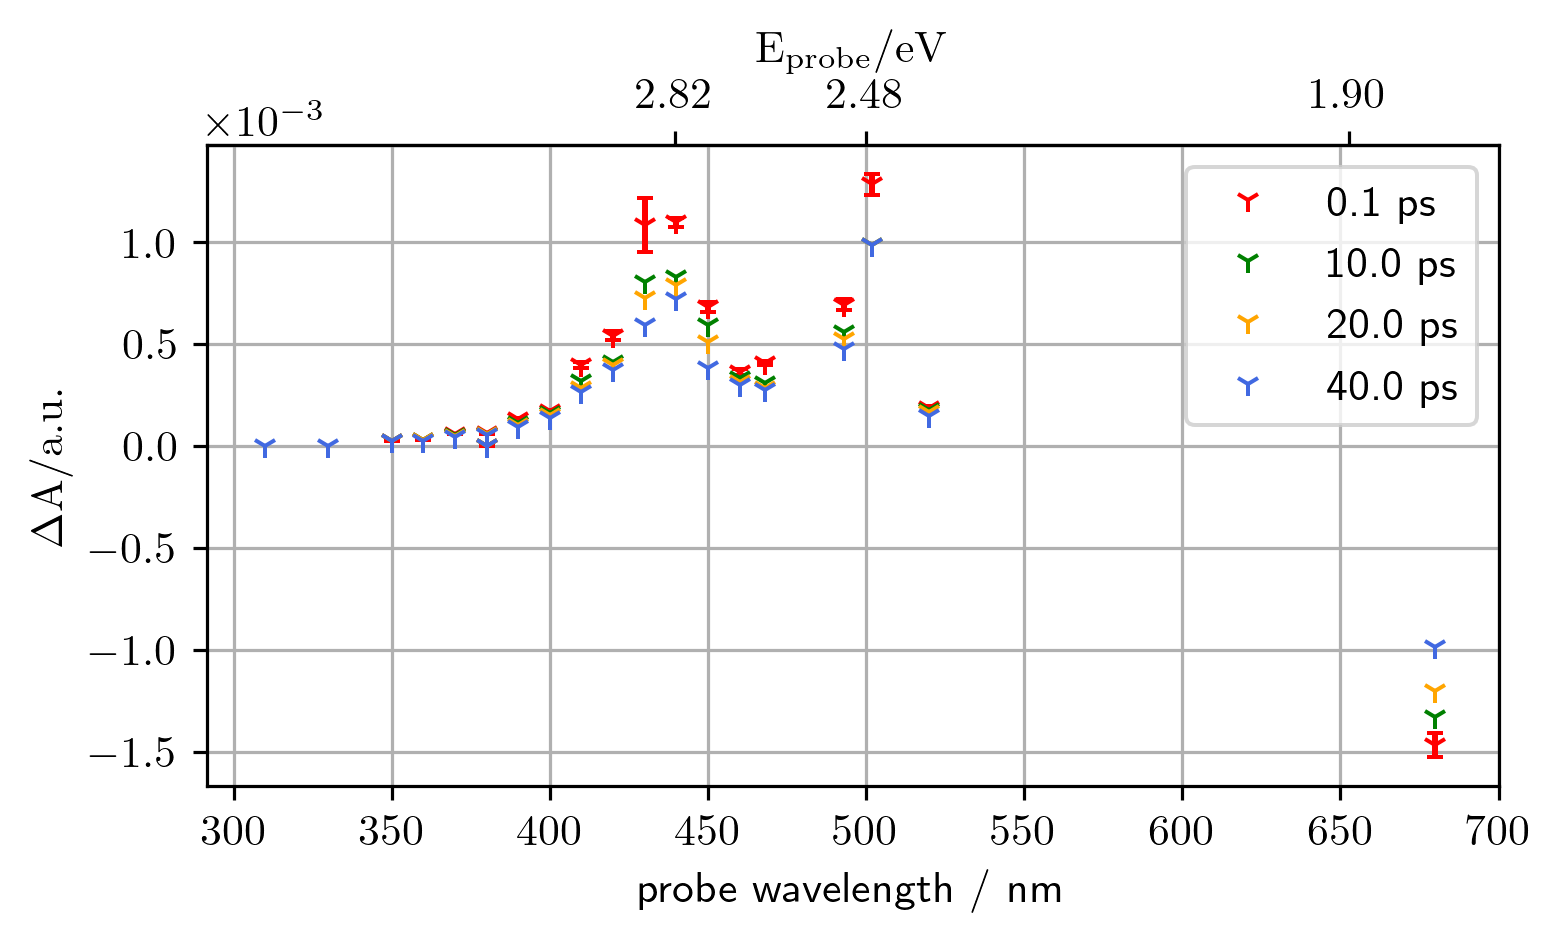
\includegraphics[scale=1]{images/TimeResolvedWavelengthScanSQIB1perc_PMMA_mapCorrected.png}
\caption{Time resolved (fitted) transient absorbance probe spectrum of 1\% SQIB PMMA. Errorbars for 0.1 ps based on peak pump radiant exposure uncertainty. Pump wavelength is 653 nm with power densities noted in tab. \ref{tab:powersWavScan}. Correction with reference map has been applied. Absorbance values calculated from (multi-)exponential decay fits.\label{fig:SQIB_PMMAwavelengthscan}}
\end{figure}

A comparison is made to data for squaraines with n-butyl sidechains by Zheng et al.\cite{Zheng2020} in fig. \ref{fig:TA_vsZheng} and a zoomed section detailing the ESA bands in fig. \ref{fig:TA_vsZheng_Zoomed}. Notably Zheng used a white light probe setup and corrected measurements for anisotropy, leading to a much finer spectrum and slightly different peaks. Due to a moving sample setup Zheng also could use far higher pump power densities, which for our measurement setup would degrade our sample too quickly to acquire a delay scan. The measurements are scaled so that the transient absorption immediately after temporal overlap at \SI{680}{\nano\meter} is -1. Reason for that is in our case the transient behaviour directly on the maximum of the CW absorption band at \SI{653}{\nano\meter} proved hard to correctly measure, which is why an off maximum measurement point was chosen to compare.%madlad used up to 80 nJ/pulse

\begin{figure}[hbtp]
\centering
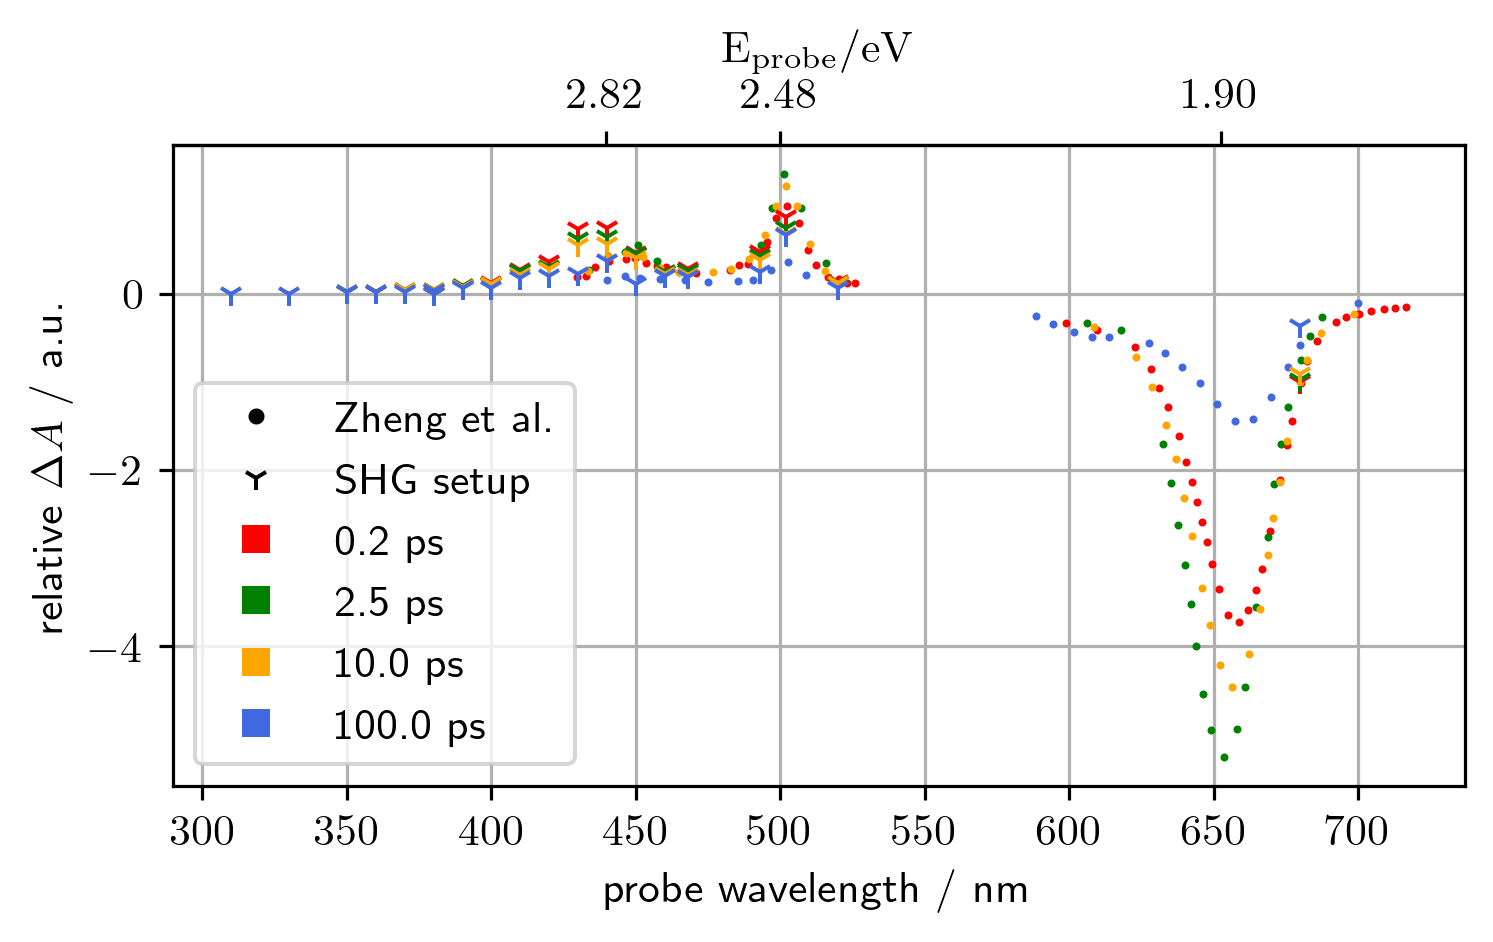
\includegraphics[scale=1]{images/wavScanVsZheng.png}
\caption{TA fits of 1\% SQIB in PMMA vs Zheng\protect\cite{Zheng2020}\\ Notably the 0.2 ps are below the chosen temporal resolution of our measurement and the 100 ps decay point is purely fit data, as the measurements do not extend past a delay of 50 ps.\\
Zheng measurement is isotropic (anisotropy corrected considering both parallel and orthogonal pump probe polarization), while ours is parallel only. Measurements are scaled so that the transient absorption immediately after temporal overlap at \SI{680}{\nano\meter} is -1.\label{fig:TA_vsZheng}}
\end{figure}

\begin{figure}[hbtp]
\centering
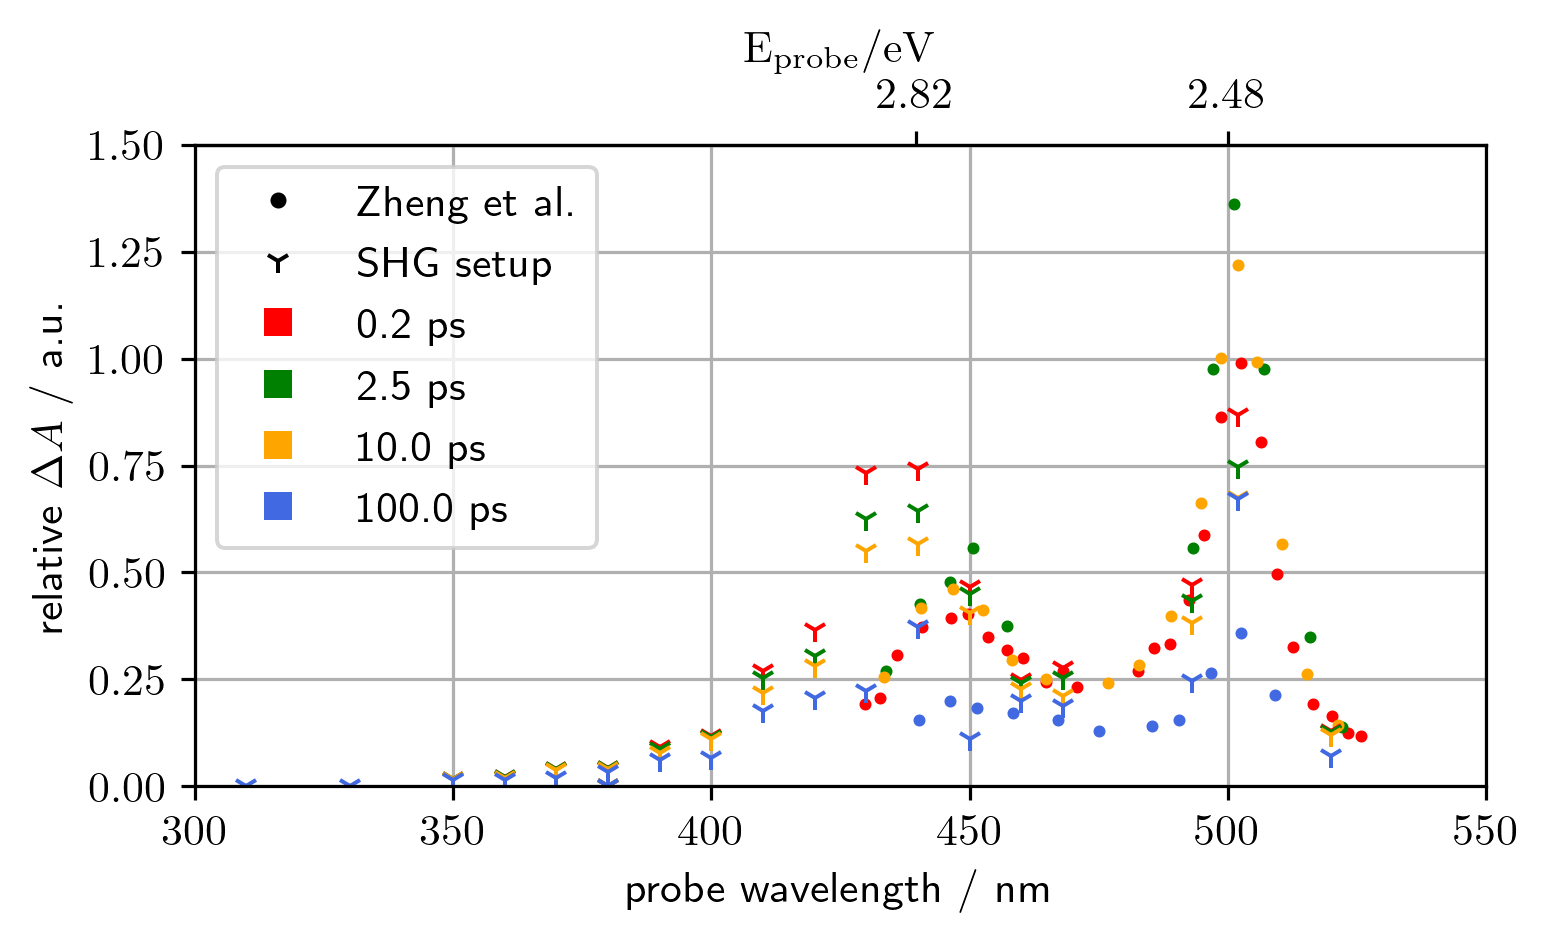
\includegraphics[scale=1]{images/TimeResolvedWavScanvsZheng_Zoom.png}
\caption{Zoomed TA fits of 1wt\% SQIB in PMMA compared to 1wt\% squaraine in PMMA by Zheng\protect\cite{Zheng2020}\\ Notably the 0.2 ps are below the chosen temporal resolution of our measurement and the 100 ps decay point is purely fit data, as the measurements do not extend past a delay of 50 ps.\\
Zheng measurement is isotropic (anisotropy corrected considering both parallel and orthogonal pump probe polarization), while ours is parallel only.Measurements are scaled so that the transient absorption immediately after temporal overlap at \SI{680}{\nano\meter} is -1.\label{fig:TA_vsZheng_Zoomed}}
\end{figure}
\textbf{mention vs Zheng scans and talk about behavior}

Additionally to the fitted behaviour in fig. \ref{fig:SQIB_PMMAwavelengthscan} the corrected data is shown "raw" in fig. \ref{fig:SQIB_PMMA_rawWavs}, where the mean response of \SI{1}{\pico\second} steps is shown relative to the absolute value of the maximum response.
\begin{figure}[htp]
\centering
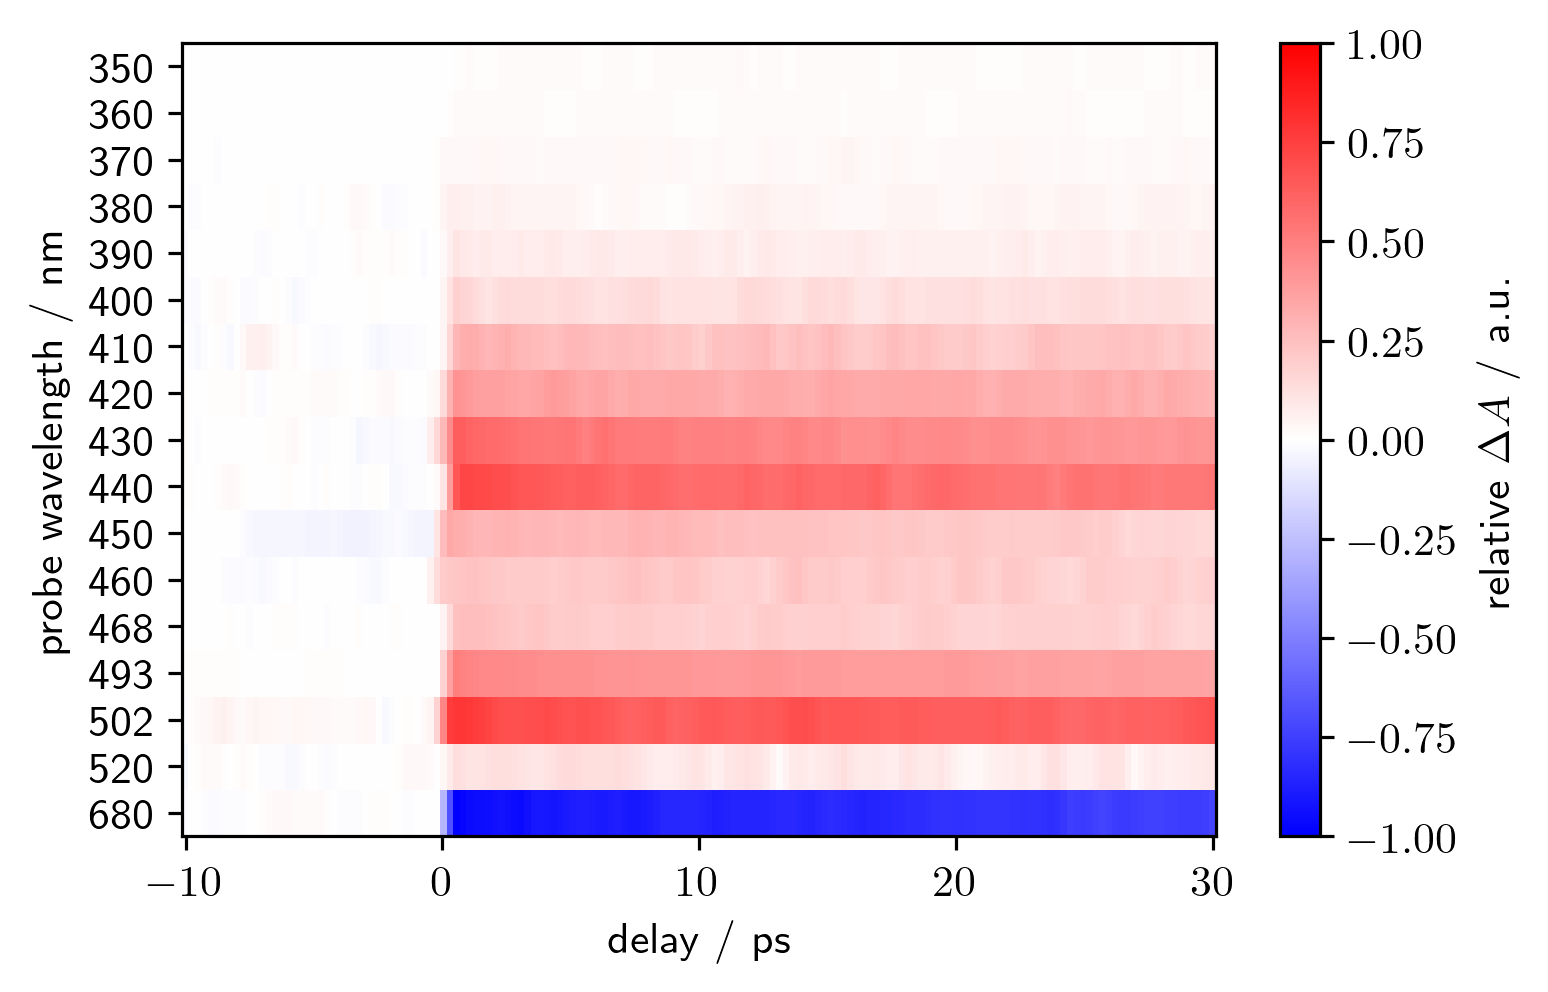
\includegraphics[scale=1]{images/RawishDataWavelengthScanSHG.png}
\caption{Alternative plot of probe wavelength scan at a 653 nm pump wavelength.\\Map correction and degradation correction applied. The data shown is a mean over several timesteps with a 1 ps stepsize. Data is aligned to their fitted pump probe temporal overlap delay.\label{fig:SQIB_PMMA_rawWavs}}
\end{figure}
\paragraph{pump and probe wavelengths}
Note again that the pump and probe pulses are not monochromatic but have an extended chromatic spectrum. Pump FWHM is expected to be in the range of \SI{23}{\nano\meter} with the centroid being \SI{653}{\nano\meter}. For the probe pulse things are slightly more complicated, where the output directly from the NOPA is straight forwards and the centroid is set to be the shown shown value. For SHG on the other hand the spectrum ahead of the cage is usually not measured, thus the wavelength noted is half the wavelength of the fundamental centroid. Keeping the fundamental intensity near the SHG threshold restricts the possible wavelength shift by phase matching. At most a shift of to the half values of the spectral distribution may be expected at high powers and less for powers near the threshold of SHG. Examples for spectra similar to the ones used in measurements are shown in fig. \ref{fig:probeSpectra}.

\paragraph{PMMA background}
A quick TA measurement for a PMMA only sample was done for a 653 nm pump with probe wavelengths of 370 nm and 440 nm,  wavelengths where PMMA is highly transmitting, and at reasonable pump powers no signal response was detected. Pushing it to unreasonable pump powers at the edge of white light generation there may be slight ESA, however at these powers the measurement technique is fundamentally flawed due to excessive stray light. This rules out the edges the long shoulder of the measurement being an effect of purely the PMMA used for the solid solution.




\chapter{Examination of reliability}\label{chpt:reliability}
Some tests have been done to ascertain the validity and stability of the corrections devised for the UV extended TAM. The same 1wt\% SQIB in PMMA sample is used for following measurements.
\section{Sample irregularities}
As mentioned above irregularities over the area of the sample probed were attempted to linearly compensate for with a reference map at a pump 653 nm probe 680 nm combination. The attempt of a linear compensation does make sense if the variation is of sample thickness but not necessarily for density variations, see sec. \ref{deriv:RadianceResponse}. In the case of drastic density variation features that are not of the plain coulombic monomer spectrum could be amplified and the states measured be quenched more quickly than for the monomer. Comparing the 1wt\% and 4wt\% graphs of the CW absorption it seems likely that a sample density variation of 100\% would be a minor influence on the transient absorption spectrum recorded, considering other uncertainties involved.

\section{Power density dependence}\label{sec:powerVar}
For measurements to be valid there should be a linear correspondence of pump power and the measured absorbance. Main concern here is that pump irradiance is within the linear regime of the transient absorption response. \textit{\textcolor{gray}{Additionally for the probe pulse it is important, that its intensity does not saturate the sample by itself leading to a GSD, which would introduce an unwelcome degree of freedom to the measurements.}} For the probe pulse the linear response of the sample is also important. In case of a too high radiance the sample may saturate as well, which can influence the response in two ways additional to processes involving more than one photon: First for a probe wavelength experiencing ESA, to simplify assume no absorption in the groundstate, the ESA response would be reduced, just like the the population transfer from the groundstate leads to GSD. Secondly, for a GSD probe wavelength it would lead to a further reduction in absorption  and an increase of the response.\\
To test this multiple pump and probe power combinations were tested, at the same sample position, only variable linear neutral density filter insertion was changed to change the attenuation. Insertion depth of the variable ND filters was assumed to not change the overlap and only the starting overlap was recorded. The linearity of the sample is shown for powers up to \SI{295e-3}{\radExp} pump and \SI{91e-3}{\radExp} probe combinations. To note is that these points were measured at the same sample spot, thus sample degradation is a factor to consider. Specifically the graph showing the probe peak radiance dependence in fig. \ref{fig:powerVarCorrection} shows sample degradation due to the high pump power density. Notably the higher power density measurements agree far more regarding degradation correction. There is no obvious reason for the low probe peak radiance measurement, corresponding to the first measurement of the three, having a slightly stronger response. The second measurement at a probe radiance of \SI{90e-3}{\radExp} responds very well to the applied degradation correction and all three sub-measurements coincide. This implies that the decreased response is not just based on faster degradation due to probe influence.

\begin{figure}[hbtp]
\begin{subfigure}[t]{0.5\linewidth}
\centering
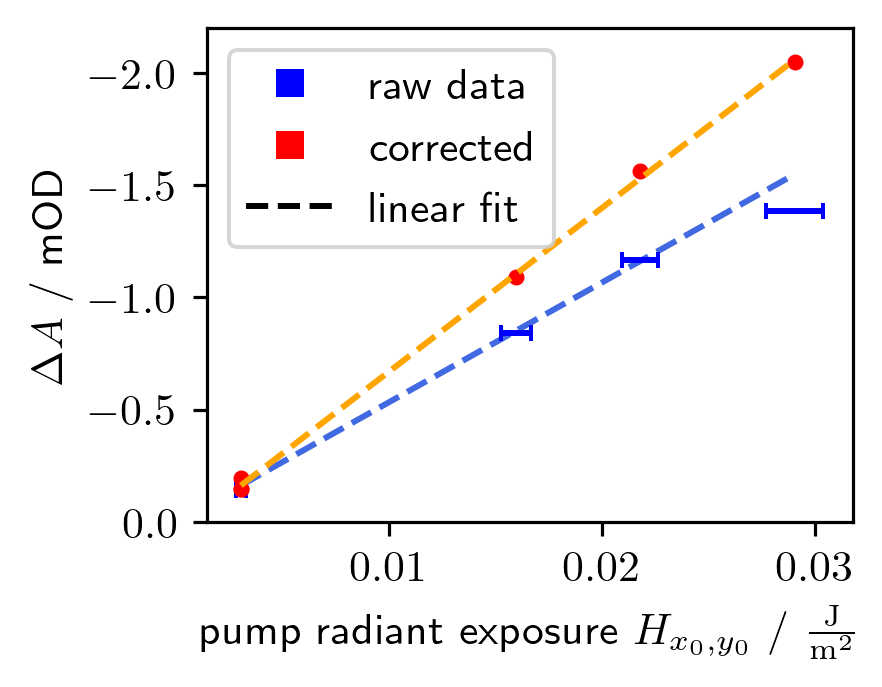
\includegraphics[width=\linewidth]{images/PowerVariationCorrectedPump.png}
\caption{Influence of variation of pump radiance on signal. At lowest pump peak radiance are three measurements with varied probe peak radiance in range of \SIrange{114e-4}{455e-4}{\radExp}, with raw data shown in fig. \ref{fig:PowerVarL}. They show a minimal spread in response.}
\end{subfigure}\hfill
\begin{subfigure}[t]{0.5\linewidth}
\centering
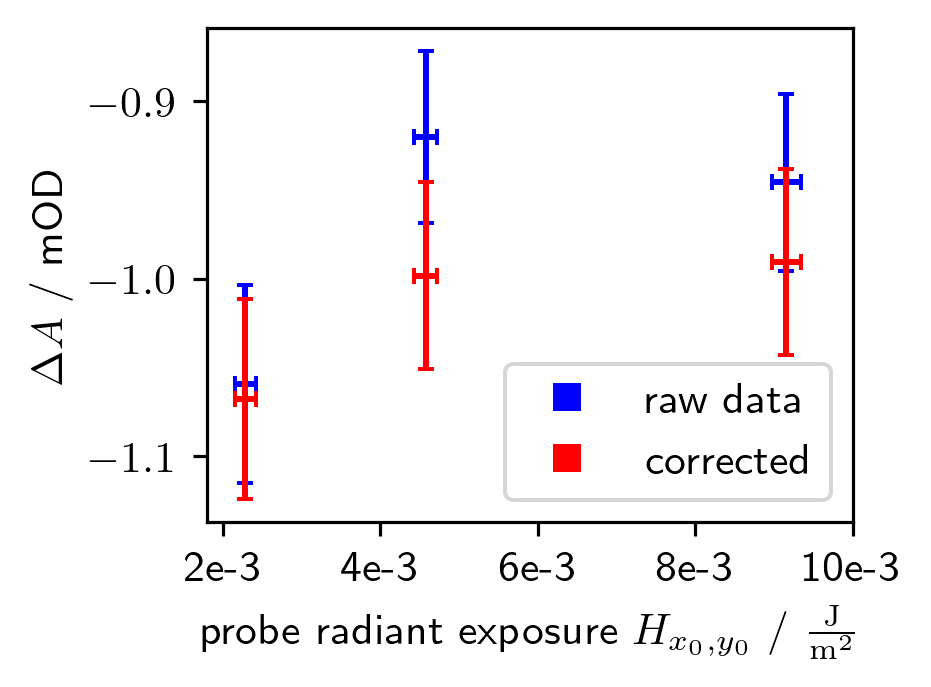
\includegraphics[width=\linewidth]{images/PowerVariationCorrectedProbe.png}
\caption{Influence of variation of probe radiance on signal at pump radiance \SI{221e-3}{\radExp}. Measurements were made in order left, right and center.\label{fig:PowerVarProbe}}
\end{subfigure}
\caption{Influence of variation of peak radiance on signal of pump 653 nm and probe 680 nm. Uncertainties based on peak radiant exposures.
Overlap corrected data in blue and additionally pump degradation corrected data in red. Every point shown is the average of a triple measurement fitted with a single exponential decay. In red the degradation compensated points are shown, only accounting for the pump peak radiance.\\ The relatively high probe intensity in the GSD band of squaraine  may be the reason for the error in degradation compensation in fig. \ref{fig:PowerVarProbe}, since the highest probe radiance is the second measurement point. \label{fig:PowerVarRaw}}
\end{figure}

\begin{figure}[hbtp]
\centering
\begin{subfigure}[t]{0.45\textwidth}
\centering
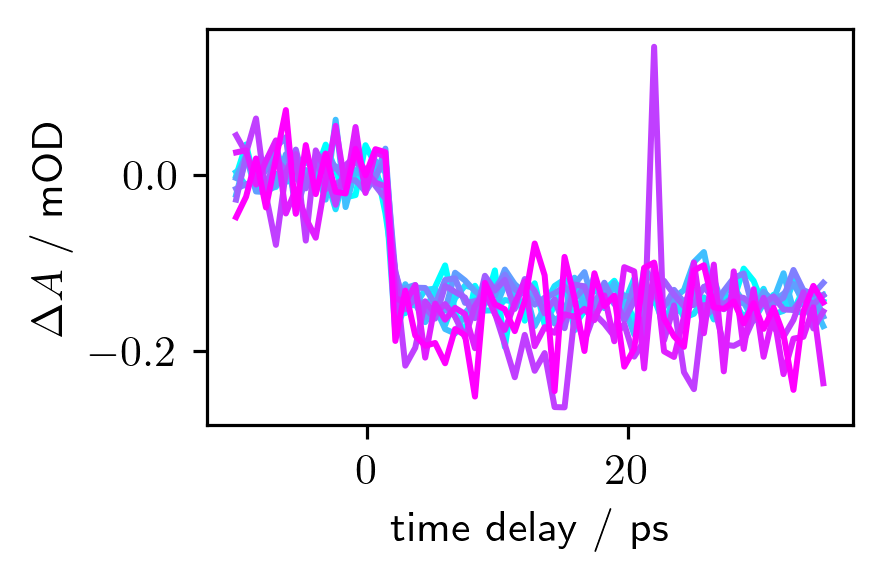
\includegraphics[scale=1]{images/PowerVarLowPumpVarProbe.png} 
\caption{Peak pump radiance \SI{31e-3}{\radExp}\\TA\_fourier measurements:\\ 6615-6620, 6630-6632\label{fig:PowerVarL}}
\end{subfigure}
\hfill
\begin{subfigure}[t]{0.45\textwidth}
\centering
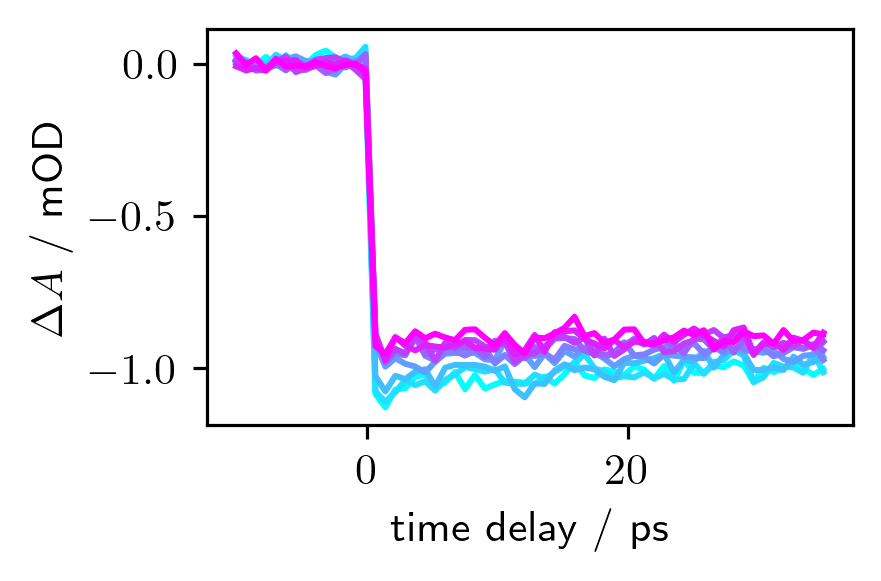
\includegraphics[scale=1]{images/PowerVarHighPumpVariedProbe.png} 
\caption{Peak pump radiance \SI{221e-3}{\radExp}\\TA\_fourier measurements:\\ 6645-6653\label{fig:PowerVarR}}
\end{subfigure}
\caption{Power variation raw transient absorption data\\
For both subplots the probe power density is varied. The influence on the decay of signal response on the right subplot is due to high powers inducing stronger degradation in the sample.}
\end{figure}

\section{Overlap correction value accuracy}
As laid out in section \ref{sec:CorrFactor} a correction factor is calculated for every measurement point to compensate error in lateral position as well as in relative size of pump and probe beam.
To check this measurements with varying overlap were taken, for which the fits can be seen in fig. \ref{fig:correctionComparison}.
Pump and probe point spread functions are measured together for every measurement, but the pump beam is not altered in any way. The corrected output is shown in tab. \ref{tab:ArtCorrTest}. 
\begin{figure}[!h]
\centering
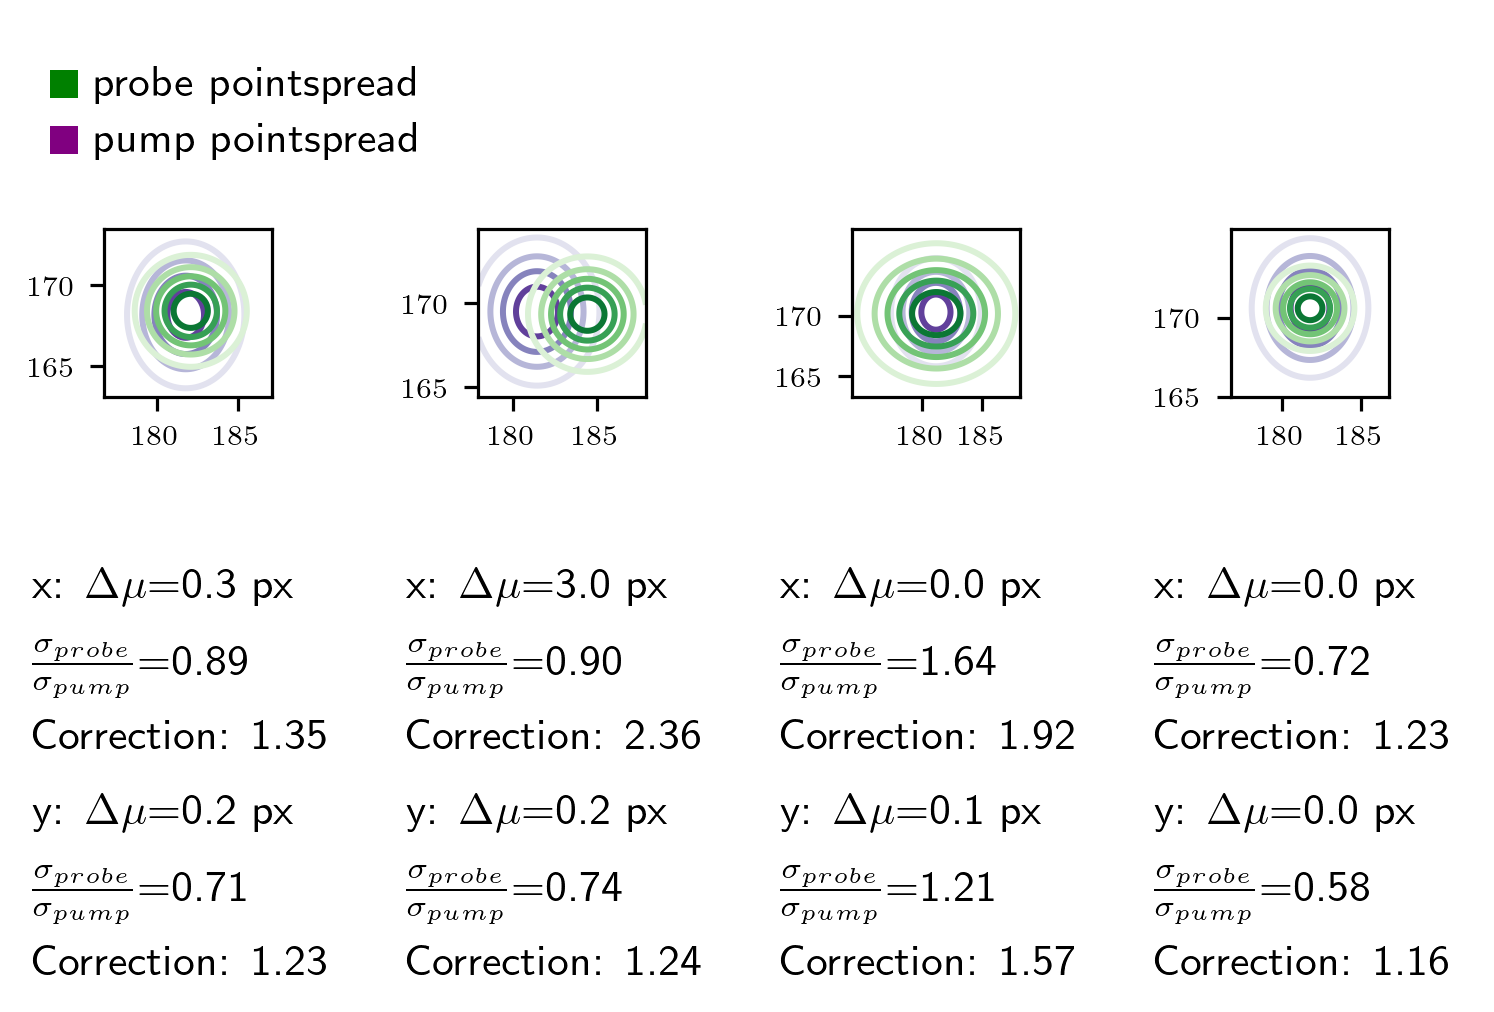
\includegraphics[width=\linewidth]{images/CorrectionComparison.png}
\caption{\textbf{fix}Beam fits plotted along with their overlap correction. Raw pointspreads can be seen in fig. ?? not sure yet\label{fig:correctionComparison}}
\end{figure}

\begin{figure}[hbp]
\centering
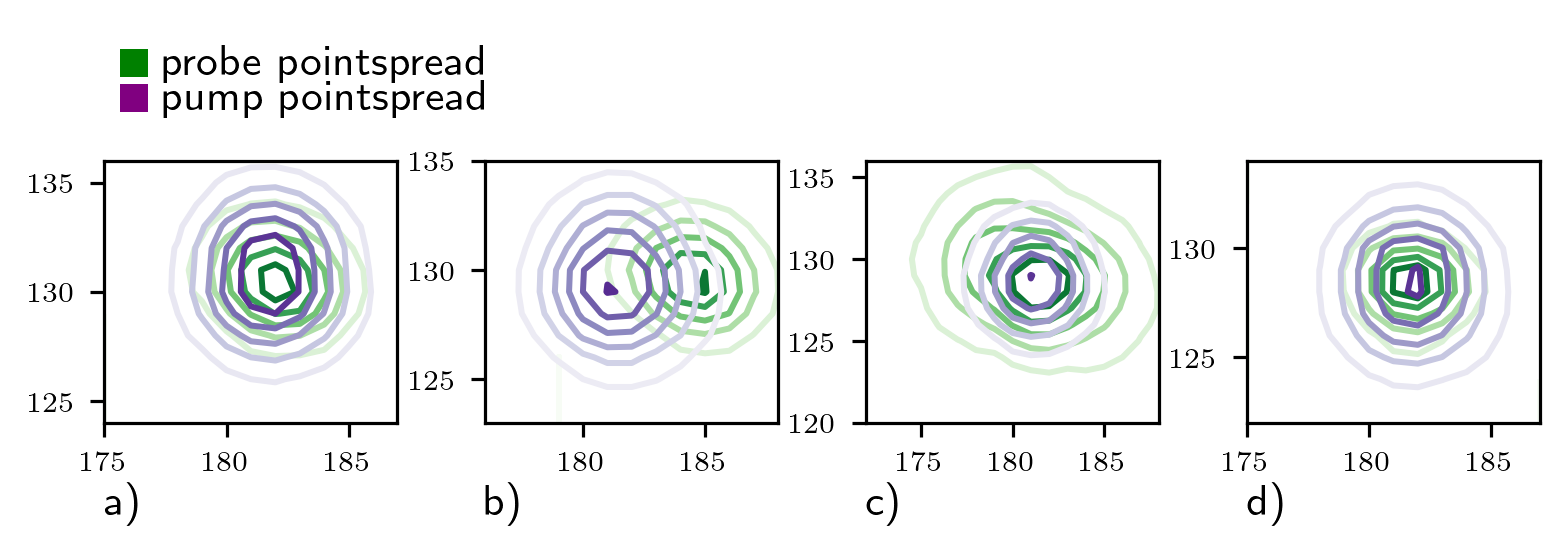
\includegraphics[scale=1]{images/CompensationTestRaw.png}
\caption{background subtracted point spreads, pump is purple, probe is green}
\end{figure}

Shifted looks fine, wide has a diagonal beamshape I am not fitting properly (fundamental problem, not sure if I want to open this can of worms or how to approach this so it is a sensible method. This would force me to use numeric methods regarding the final overlap, since the axes )
\begin{table}[!hb]
\caption{Calculated corrected values from fitted biexponential decay at time 0\\ uncertainty of dOD fits is not included, maybe only do uncertainty of dOD fits\label{tab:ArtCorrTest}}
\begin{tabular}{llllll}
x$\sigma_1/\sigma_2$ / px & y$\mathrm{\Delta}\mu$ / px & x$\mathrm{\Delta}\mu$ / px & y$\mathrm{\Delta}\mu$ / px & $\Delta OD$ / $mOD \cdot \frac{W}{m^2}^{-1}$ & \begin{tabular}[c]{@{}l@{}}uncertainty\\ (missing dOD uncertainty)\end{tabular} \\
$0.89 \pm 0.02$           & $0.71 \pm 0.01$            & $0.31 \pm 0.05$            & $0.25 \pm 0.02$            & $7.6 \cdot 10^{-4}$             & $2.3 \cdot 10^{-4}$                                                             \\
$0.90 \pm 0.02$           & $0.74 \pm 0.01$            & $3.00 \pm 0.05$            & $0.15 \pm 0.02$            & $4.5 \cdot 10^{-4}$             & $1.6 \cdot 10^{-4}$                                                             \\
$1.64 \pm 0.04$           & $1.21 \pm 0.02$            & $0.03 \pm 0.05$            & $0.12 \pm 0.04$            & $6.7 \cdot 10^{-4}$             & $2.6 \cdot 10^{-4}$                                                             \\
$0.72 \pm 0.02$           & $0.58 \pm 0.01$            & $0.00 \pm 0.04$            & $0.02 \pm 0.02$            & $7.2 \cdot 10^{-4}$             & $2.8 \cdot 10^{-4}$                                                            
\end{tabular}
\end{table}

\section{Sample degradation}\label{sec:degradation}
The main loss of sample response is suspected to be dependent on the pump pulse, as it is right at the CW absorption peak. A repeated delay scan at the same position is shown in fig. \ref{fig:rawDegradation} to show degradation behavior. That combined with the higher peak radiance of the pump pulse makes it the prime candidate of photo bleaching. This also would be supported by the circumstance, that a pump probe wavelength combination fully on the main absorption peak always showed a lower GSD response than expected. Reasoning for that is an extremely fast degradation of the sample spot where pump and probe coincide in their peak radiances.\\
The pump pulse on the main absorption peak is expected as the main degrading component for most of the probe spectrum as long as low probe peak radiances are used. For high probe photon energies this may no longer be the case, however from the spectra recorded so far no indication of a strong influence is seen.\\
Thus reduction of transient response at a pump peak radiance of \SI{79(4)e-3}{\radExp} at 653 nm combined with a probe wavelength of 493 nm at \SI{8.6(1.3)e-3}{\radExp}, which is close to the main absorption peak of the first ESA transition of the monomer. The time dependence is taken as a series of typical measurements, as the pump pulse is expected to be the main influence and not the pump probe interaction. This mainly serves to confirm the typical measurement behaviour and to make an attempt at correcting for the response loss due to photo bleaching.

\begin{figure}[hbtp]
\centering
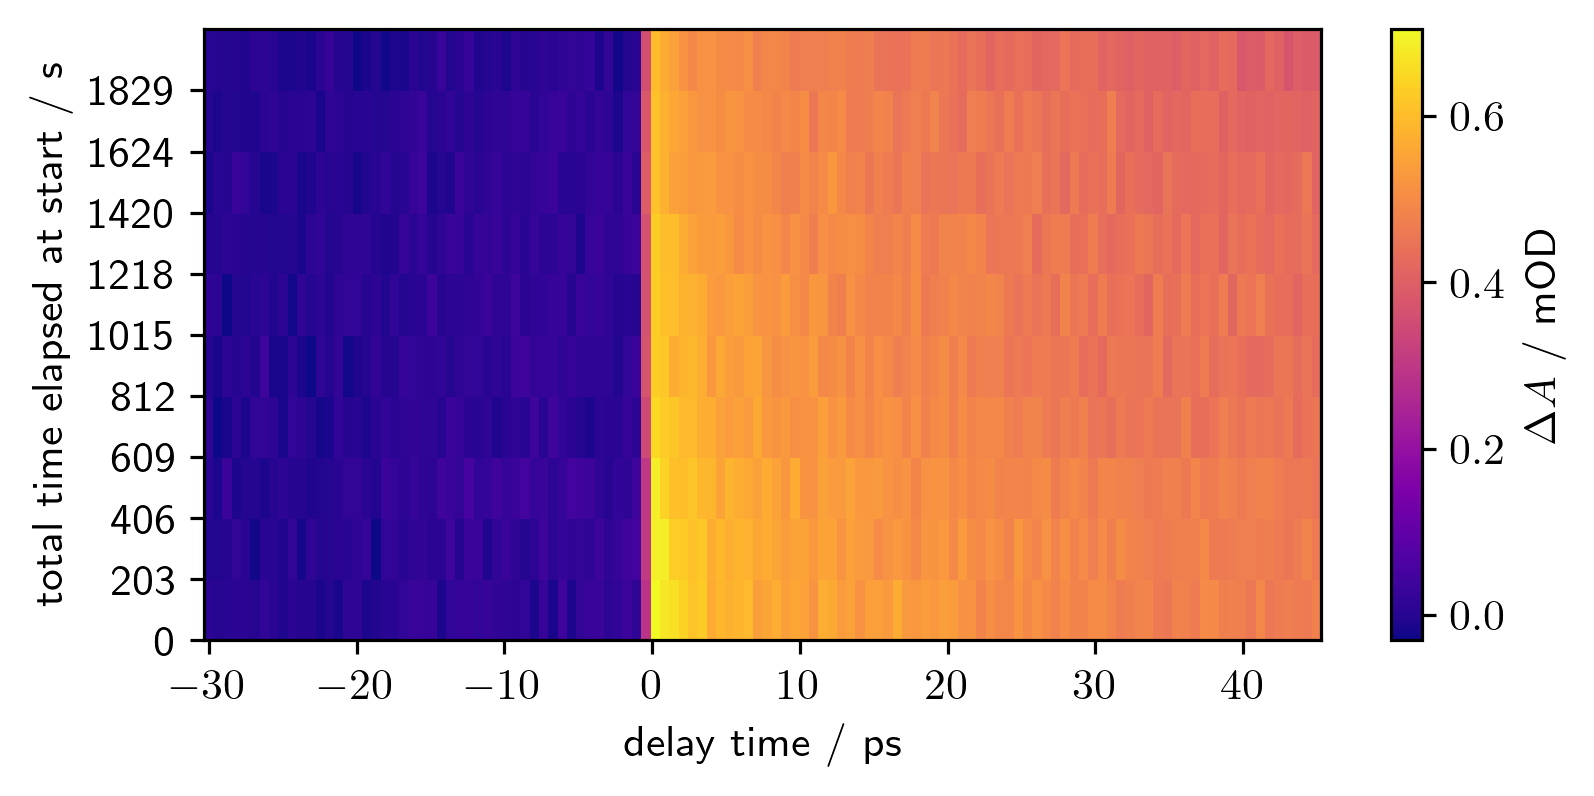
\includegraphics[width=\linewidth]{images/DegradationRAWPump653Probe493.png}
\caption{Raw data from degradation series of identical measurements at same spot at pump \SI{653}{\nano\meter} \SI{79(4)e-3}{\radExp} and probe \SI{493}{\nano\meter} \SI{8.6(1.3)e-3}{\radExp}.\\
Time at start on the y axis corresponds to the starting time of the measurement\label{fig:rawDegradation}}
\end{figure}
Usually photobleaching is modelled as an exponential decay as a function of time exposed. A fit is made to the decay of the absorbance $\frac{A\left(t\right)}{A\left(t=0\right)} = exp(-\frac{t}{\tau})$.
All datapoints, which are background subtracted, after the temporal overlap are used in fitting. This avoids strong variations in the pre temporal overlap area, where the absorbance values vary mildly around 0 mOD leading to a strong variation of their ratio and an ill-conditioned fit. A nonlinear least squares approach with numpy curve\_fit is used to minimize a residual defined as
\begin{equation}\label{eq:degradationFitting}
\mathrm{residual} = \sum_{t_{start,i},d_j} \left(ln\left(\lvert\frac{\Delta A(t_{start,i},d_j)}{\Delta A(t=0,d_j)}\rvert\right)- \frac{t_i}{\tau}\right)^2
\end{equation}
Here $t_i$ is the time at the start of the scan, $d_i$ is the delay between pump and probe pulses and $\tau$ is the decay parameter fitted. The absolute value of change in absorbance is taken to avoid negative values in the logarithm, even though they are unlikely when only $d_i$ after temporal overlap are used.  This simplification is needed as only starting times of delay scans are collected. A moving mean may be used to smooth particularly noisy data. Used fits use a moving mean of 5 measurement points. Comparison to no smoothing mean does not change the fit result in a significant way, though the data is not particularly noisy.\\
The correction applied to the delay scans assumes an equal time for each measurement point based on the mean time between two delay scans and the number of points in the scan. The equation equivalent to the compensation is shown in eq. \ref{eq:degradationCompensation}. In fig. \ref{fig:degradationCorrectionComparison} a comparison of raw and corrected data is shown. The decay corrected data shows a far lower spread in absorbance values making the fitting method a valid option. 

\begin{equation}\label{eq:degradationCompensation}
A_{compensated}(t_i(d_j), d_j) = A(t_i(d_j), d_i)\cdot exp\left(+\frac{t_i(d_j)-t0}{\tau_{1/e}}\right)
\end{equation}

\begin{equation*}
t_i(d_j) = t_i + j\cdot \mathrm{mean(\Delta t_{delay scan)}}
\end{equation*}

\begin{figure}[hbtp]
\centering
\begin{subfigure}[t]{0.4\linewidth}
\centering
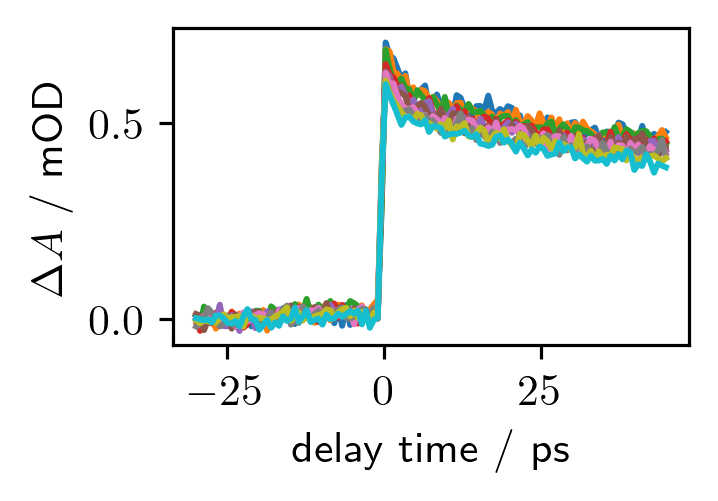
\includegraphics[scale=1]{images/DegradationRAWPump653Probe493-Graph.png}
\caption{Raw data as in fig. \ref{fig:rawDegradation}}
\end{subfigure}
\hfill
\begin{subfigure}[t]{0.4\linewidth}
\centering
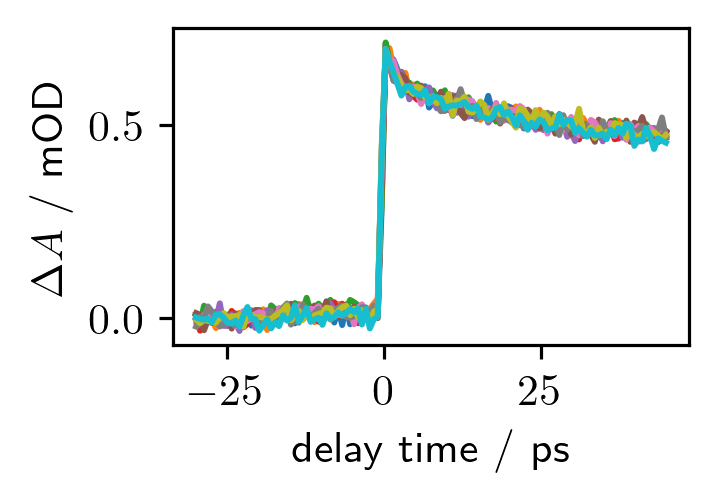
\includegraphics[scale=1]{images/DegradationCorrectedPump653Probe493-Graph.png}
\caption{Exponential decay corrected data\\
Decay constant $\tau_{1/e}$ = \SI{14100}{\second} at \SI{79(4)e-3}{\radExp}}
\end{subfigure}
\caption{Comparison of raw data and decay corrected data for measurements TA\_fourier: \mbox{6778 - 6787}.\label{fig:degradationCorrectionComparison}}
\end{figure}



\begin{figure}[hbtp]
\centering
\begin{subfigure}[t]{0.3215\linewidth}
\centering
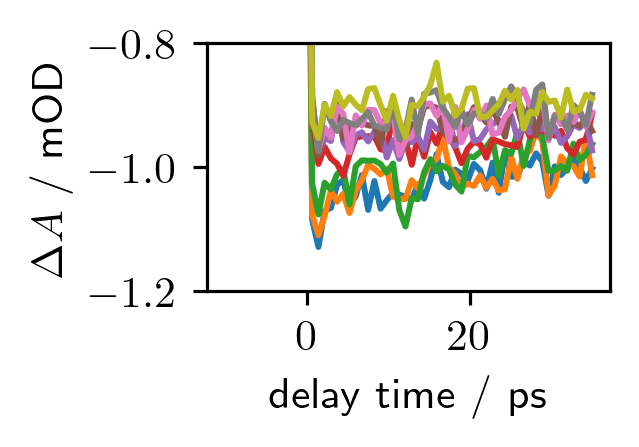
\includegraphics[width=\columnwidth]{images/PowerVarHigh_Raw.png}
\caption{Raw data as in fig. \ref{fig:PowerVarR}}
\end{subfigure}
\hfill
\begin{subfigure}[t]{0.3215\linewidth}
\centering
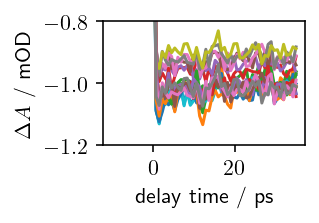
\includegraphics[width=\columnwidth]{images/PowerVarHigh_CorrNative7800.png} 
\caption{Corrected per native fit at $\tau_{1/e}=$\SI{7800}{\second}}
\end{subfigure}
\hfill
\begin{subfigure}[t]{0.3215\linewidth}
\centering
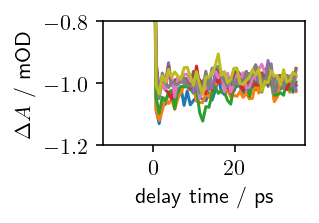
\includegraphics[width=\columnwidth]{images/PowerVarHigh_CorrEstimate14100_2.8.png} 
\caption{Corrected from degradation fit fig. \ref{fig:degradationCorrectionComparison}\\
$\tau_{1/e}=$\SI{14100}{\second}, $P_{ratio}=\frac{P_{\SI{680}{\nano\meter}}}{P_{\SI{497}{\nano\meter}}} = \frac{221}{19}= 2.8$}
\end{subfigure}
\caption{Comparison of pump \SI{653}{\nano\meter} probe \SI{680}{\nano\meter} raw, corrected by direct fit and corrected by applying the decay constant gathered from fig. \ref{fig:degradationCorrectionComparison}\\Applying the power correction as a ratio factor of used measurement power density divided by fitting power density as follows $\Delta OD(t) = \Delta OD(t=0)\cdot e^{\frac{t\cdot P_{ratio}}{\tau}}$, where $P_{ratio} =1$ if the power density is the same as for the measurement where degradation is fitted and t is the elapsed times since start of the measurement. Note that the measurements gathered here have different probe power densities.\label{fig:powerVarCorrection}}
\end{figure}
\paragraph{Probe wavelengths}
Note that the probe wavelengths compared here correspond to different processes within the molecules. The degradation of the first ESA transition corresponds to an effect of inactivation of the excited state reachable from the pumped state or to a reduction of molecules which can be pumped. The GSD measurement instead just directly measures the reduction in squaraine absorption, with the probe wavelength likely just adding to the pump power of degradation with a weighting factor of the different absorption cross-section. If their degradation times coincide then the likelihood of the degradation pathway is relatively high. Additionally the probe wavelength may also introduce another degradation pathway or mediate a faster degradation via the same pathway as the GSD pathway. The single exponential degradation is only justified by it seemingly providing a decent output as well as the use case and measurement data not warranting better modelling. A description of different pathways for organic fluorophores may be found along with behaviors, however they strongly vary for different molecules making them unpredictable for untested molecules.\cite{Demchenko_2020}

\paragraph{Power dependence}
A simple naive assumption for power dependence of photobleaching is same bleaching for same total dose. This ignores photobleaching pathways and power density dependencies. It is unknown if this is applicable for the used peak powers, since references for other fluorophores usually used CW methods and pulsed operation with similarly high peak powers may well behave differently. Since the actual power dependence here is beyond the scope of the paper the naive assumption is attempted. Here the dependence of photo degradation is a direct product of the power density on the exposure time, for total dose the sample is exposed to, $e^{-\frac{t\cdot P}{\tau}}$, where $t$ is the exposure time and $P$ is the power density.\cite{Eggeling1998}

A comparison of the degradation in the measurements in fig. \ref{fig:degradationCorrectionComparison} with a probe wavelength of \SI{497}{\nano\meter} and fig. \ref{fig:powerVarCorrection} is made, to show the decreased spread of the corrected data.

Another aspect to consider is the power density influence on degradation, for which the measurements from sec. \ref{sec:powerVar} are used.  Their decay constant shows $\tau_{1/e}\left(\SI{221e-3}{\radExp}\right)=$\SI{7600}{\second}  opposed to the $\tau_{1/e}\left(\SI{79e-3}{\radExp}\right)=$\SI{14100}{\second}. The fit from the degradation series, when corrected for total dose rate, seems to fit better with all measurements close together, while the fit made on the power variation measurements leads to a lot wider spread. The effect of the constants on the measurements is shown in fig. \ref{fig:powerVarCorrection}.

A not so naive model for degradation would need to account for the beam shape and overlap of pump and probe beams, as this would change sensitivity according to the pump intensity profile, which in turn would increase relative response near the FWHM of the pump beam profile. The high power density area on the sample however would also decay quicker, because photodamage tends to be at least linearly dependent on the total dose.


\chapter{In depth software description}
\section{Beam characterisation}
\subsubsection{Inner workings Artray camera interactions}
The software package is based on the SDK provided freely by Artray in C\#, specifically on the CS.NET\_Graphic example software. 

\paragraph{raw data output}
Data is handled as one dimensional byte arrays by the SDK and has to be processed into a workable format. The camera specifications allow for a maximum bit depth of 12 bit. To be able to access this bit depth the video format of "Color 48bit*" has to be set, as the monochrome formats do not allow higher bit depth. Adjusted software by the manufacturer was attempted, but abandoned on our side due to troubleshooting issues. The single pixel data for the "Color 48 bit*" setting is encoded as 2 byte per colour channel per pixel. Since, even though this is a monochrome camera, the colour output was not the same colour values for all returned subpixel types, meaning RGB, the saturation of the camera was set to be minimal in software (-255). This leads to identical red, green and blue subpixel values. From these 3 colour values red is arbitrarily chosen for further processing.
The data formatting is explained with the help of fig. \ref{fig:ByteArtrayOut}. Both bytes are formatted as big endian or most significant bit first. The second byte holds the most significant bit, with the first hex value and thus 4 bits being empty. The first bit holds the remaining 8 bit of the 12 bit value.

\begin{figure}[hbtp]
\centering
\includegraphics[scale=1]{images/ArtrayByteImage.png}
\caption{Data scheme of periodic byte structure of artray output with hexadecimal placeholders\\
$\mathrm{H_{22}}$ holds the 4 most significant bit and byte 1 is simply appended\\
$\mathrm{0_{21}}$ of byte 2 is always empty.\label{fig:ByteArtrayOut}}
\end{figure}

The via bitwise operations processed value is then assigned to a short integer array. Notably for processing the region of interest (ROI) needs to be known. It is not included in any of the raw data itself.

\section{Useful methods available}
A short listing of python programs and methods used for analysis of data that are useful intended to point to available software for future use: \textbf{this may be replaced with just be a link to a github page with permanent access and a good readme}
\subsection{fileParsingMethods}
\paragraph{parseFilenames} is used to easily parse TA_fourier filenames along with saturation files into a list of full path TA_fourier files which can be handed to any function taking arrays of filenames.
\paragraph{parseSummaryFileToArray} uses "parseFilenames" to return either transient absorbance or transient transmissivity along with a single delay vector, files must have same delay vector. Possible to remove a linear background by fitting if needed. Alternatively similar function returning the raw intensity vectors along with a delay vector is "parseSummaryFiletoRaw".
\paragraph{getTimes} is used get starting times of TA_fourier files or saturation summary files. TA_fourier file compatibility may be broken by any matlab release changing the header of .m files.
\subsection{SeriesDegradation}
\paragraph{autoCompensation} is used to automatically calculate correction values to for known degradation constant and power for a filename array. Returns transient absorption and transmission corrected for background, which may be linear or static, along with an array of correction factors to be applied and a delay vector. Alternatively "degradationCompensation" calculates only the correction factors from degradation constant, power ratio and number of decay steps.
\paragraph{plotTrend} shows a map of the transient absorbances of a filename array against a delay vector. 
\paragraph{fitDegradation} fits degradation of the sample according to eq. \ref{eq:degradationFitting}. Allows for smoothing with a moving mean for noisy data. Needs proper t0 index of temporal pump-probe overlap to work.
\subsection{ArtrayEvaluatorFunctions}
\paragraph{runRoutineJSON} is used to quickly rerun a fit from the summary JSON. Useful to check if something was changed in the summary. \textbf{check again, compare to ArtFit}
\subsection{ShowDelayScan} includes methods to quickly plot raw data from either a filename array or from raw data.
\subsection{ImageAnalysis} is used to show an image scan with a subtracted background. It is a direct transcription of the matlab method.
\subsection{ArtrayAnalysis}
A few ArtFit classmethods that are externally accessible and useful:
\paragraph{parseFitFile} returns a usable array of fitdata from fitdata file saved with ArtFit.
\paragraph{calculateOverlap} calculates the LiveFitting overlap that is one if pump and probe are identical.
\paragraph{calculateOverlapCorrection} calculates the correction factor for one dimension which multiplies onto the absorbance value.
\paragraph{rerunFromJSON} runs files from summary JSON file again to allow a comparison between current fitting and past fitting. Allows overwriting of summary JSON.
\chapter*{Used materials}
\begin{longtable}{p{0.48\textwidth}p{0.48\textwidth}}
    \caption{List of devices used}
    \label{tab:devices} \\
    \toprule 
    Title & Remarks \\
    \midrule
    \endfirsthead
    \toprule 
    Title & Remarks \\
    \midrule
    \endhead
    \midrule
    Continued on next page
    \endfoot
    \bottomrule
    \endlastfoot
    Light Conversion PHAROS & Yb:KGW femtosecond laser, PH1-20-0400-02-30, L191103; \SI{40}{\kilo\hertz} repetition rate at \SI{400}{\micro\joule} pulse energy \\
    Light Conversion ORPHEUS N-3H & NOPA, $ \lambda = \SIrange{500}{950}{\nano\meter} $ \\
    Light Conversion ORPHEUS N-2H & NOPA, $ \lambda = \SIrange{640}{950}{\nano\meter} $ \\
    Scitec 310 CD with 300CD200HS & Optical chopper, frequency $\approx \SIrange{1000}{55000}{\hertz}$, focusing on chopper wheel using two $f=\SI{125}{\milli\meter}$ plano-convex N-BK7 lenses \\
    Scitec S310Sync synchroniser & Phase and frequency locking of the chopper to external sources (function generator, laser sync output, frequency divider) \\
    Thorlabs AHWP05M-600 & \SIrange{400}{800}{\nano\meter} achromatic $\frac{\lambda}{2}$ plate \\
    Thorlabs AHWP10M-980 & \SIrange{690}{1200}{\nano\meter} achromatic $\frac{\lambda}{2}$ plate \\
    Thorlabs NExxA series, Thorlabs NDxxA series, Eksma Optics 240-25xx series & Reflective and absorptive neutral density filters, used for coarse power setting \\
    Reflective variable neutral density filters & Used to set input power exactly \\
    BG39, UG5 glass filters \\
    Thorlabs FESH0700, Newport FS-SWF set & Sputtered short-pass filters \\
    Thorlabs FELH0700 & Sputtered long-pass filter \\
    Thorlabs WP25M-UB & Ultra-broad wire grid polariser \\
    Film polarisers (not really) & For visible imaging microscopy \\
    Olympus UPlan FL N 10x & Focussing objective, 10x magnification, NA=0.3 \\
    Nikon Plan 10/0.3 160/0.17 & Imaging objective, 10x magnification, NA=0.3 \\
    EKSMA 110-1216E & plano-convex UVFS lenses\\
    mounted prism & UV translucent, unknown model\\
    Linos HighLED White & For visible imaging microscopy \\
    Sample illumination LED ring & 658 nm (measured), LT3080 current regulation for 12 V input \\
    The Imaging Source DMK 42AUC03 & Monochrome camera, particularly for spatial overlap alignment, beam shape characterization and orientation on the sample \\
    Artray ARTCAM-092UV-WOM & UV sensitive CMOS camera, used for spatial overlap\\
    Detector A & High-speed optical detectors based on Hamamatsu S1336-8BQ photodiode, JFET operational amplifiers, an analogue  long-pass filter for signal elongation and impedance converters for calibration \\
    Picoscope 5442D & Oscilloscope used for data collection from optical detectors \\
    Coherent LabMax Pro & Pulse measuring head, used for optimizing OPA output \\
    Coherent FieldMate with OP2-VIS measuring head & Laser power meter, used for setting input power, partially damaged leading to higher low intensity readings (SN: 1019L08R) \\
    Newport LTA-HS & Delay stage actuator \\
    Thorlabs Z825B, KDC101 & Microscopy sample stage actuators (horizontal and vertical) \\
    Various aluminium mirrors & Planar and concave (for focussing onto detectors) \\
    74HC73 & Dual JK flip-flop for frequency division
\end{longtable}
\begin{longtable}{p{0.48\textwidth}p{0.48\textwidth}}
    \caption{List of software used}
    \label{tab:devices} \\
    \toprule 
    Title & Remarks \\
    \midrule
    \endfirsthead
    \toprule 
    Title & Remarks \\
    \midrule
    \endhead
    \midrule
    Continued on next page
    \endfoot
    \bottomrule
    \endlastfoot
    Spectrometer software spectraLight & Light Conversion; malfunctioned with update and superseded by Waves \\
    Spectrometer software Waves & BROADCOM; Version 2.2.2.0\\
\end{longtable}

\chapter{Derivations of formula}
\section{Product of two Gaussians}\label{GaussiansDerivation}
This calculation has been cross checked with Bromiley.\cite{Bromiley2014}\\
Begin with two Gaussian distributions $\mathrm{G_1(x)\ and \ G_2(x)}$ and combine the exponential terms.
\begin{equation*}
\begin{split}
G_{12}(x) & =  G_1(x) \cdot G_2(x) \\ 
& = \frac{1}{2\pi \sigma_1 \sigma_2}
exp\left(-\frac{1}{2}\left[\frac{\left(x-\mu_1\right)^2}{\sigma_1^2} + \frac{\left(x-\mu_2\right)^2}{\sigma_2^2} \right]\right)
\\
& = \frac{1}{2\pi \sigma_1 \sigma_2} exp \left(-\frac{1}{2\sigma_1^2 \sigma_2^2} \left[
\sigma_2^2 \left(x^2 - 2 \mu_1 x + \mu_1^2 \right) + 
\sigma_1^2 \left(x^2 - 2 \mu_2 x + \mu_2^2 \right)
\right] \right)
\\
& = \frac{1}{2\pi \sigma_1 \sigma_2} exp \left(-\frac{1}{2\sigma_1^2 \sigma_2^2} \left[
x^2(\sigma_1^2+\sigma_2^2) - 2x(\mu_1\sigma_2^2 + \mu_2\sigma_1^2) + (\sigma_1^2 \mu_2^2 + \sigma_2^2 \mu_1^2)
\right] \right)
\end{split}
\end{equation*}
Simplify by dividing by the following substitution and add a zero $0 = \epsilon - \epsilon$ into the exponential function.
\begin{equation*}
\sigma_{12} := \sqrt{\sigma_1^2+\sigma_2^2}
\end{equation*}
\begin{equation*}
G_{12}(x) = \frac{1}{2\pi \sigma_1 \sigma_2} exp \left(-\frac{\sigma_{12}^2}{2\sigma_1^2\sigma_2^2}\left[
x^2 - 2x\frac{\mu_1\sigma_2^2+ \mu_2\sigma_1^2}{\sigma_{12}^2} + \frac{\sigma_1^2\mu_2^2 + \sigma_2^2\mu_1^2}{\sigma_{12}^2}
+ \epsilon - \epsilon
\right]\right)
\end{equation*}
Now find $\epsilon$ to fulfil the binomial theorem $x^2- 2xb + \tilde{b}^2 + \epsilon - \epsilon= (x-b)^2 - \epsilon$ within the exponent, where $\epsilon$ is used to compensate such that $\mathrm{b^2 = \tilde{b}^2 + \epsilon}$.
\begin{gather*}
\left(\frac{\mu_1 \sigma_2^2 + \mu_2\sigma_1^2}{\sigma_{12}^2}\right)^2 \stackrel{!}{=} \frac{\sigma_1^2\sigma_2^2 + \sigma_2^2\mu_1^2}{\sigma_{12}^2} + \epsilon
\\
\begin{split}
\epsilon \cdot \sigma_{12}^4  & = \mu_2^2\sigma_1^4 + \mu_1^2\sigma_2^4 + 2\mu_1\mu_2\sigma_1^2\sigma_2^2 - \sigma_1^2\mu_2^2(\sigma_1^2+ \sigma_2^2) - \sigma_2^2\mu_1^2(\sigma_1^2+ \sigma_2^2)\\
& = - (\mu_1^2\sigma_1^2\sigma_2^2 + \mu_2^2\sigma_1^2\sigma_2^2 - 2 \mu_1\mu_2\sigma_1^2\sigma_2^2)\\
& = - \sigma_1^2\sigma_2^2(\mu_1-\mu_2)^2
\end{split}
\end{gather*}
Now one can return to $\mathrm{G_{12}(x)}$ and insert the found value for epsilon. With this the exponential function can be split into a part dependent on x and one independent of it.
\begin{equation*}
G_{12}(x) = \frac{1}{2\pi\sigma_1\sigma_2}\cdot exp\left(- \frac{\sigma_{12}^2}{2\sigma_1^2\sigma_2^2\sigma_{12}^4}\sigma_1^2\sigma_2^2\left(\mu_1-\mu_2\right)^2
\right) \cdot
exp\left(-\frac{\sigma_1^2+\sigma_2^2}{2\sigma_1^2\sigma_2^2} \left[x - \frac{\mu_1\sigma_2^2+\mu_2\sigma_1^2}{\sigma_{12}^2}\right]^2 \right)
\end{equation*}
Simplifying the equation using the substitutions that specify the $\sigma$ and $\mu$ of the combined Gaussian distribution:
\begin{gather*}
\sigma_{new} := \frac{\sigma_1\sigma_2}{\sigma_{12}}\\
\mu_{new} := \frac{\mu_1\sigma_2^2+ \mu_2\sigma_1^2}{\sigma_{12}^2}
\end{gather*}
With these the combined Gaussian can be split into a "classical" Gaussian part and a scaling parameter $S_{12}$.
\begin{gather*}
\begin{split}
G_{12}(x) & = \frac{1}{\sqrt{2\pi}\sigma_{new}}\frac{\sigma_{new}}{\sqrt{2\pi}\sigma_1\sigma_2}\cdot exp\left(- \frac{\left(\mu_1-\mu_2\right)^2}{2\sigma_{12}^2}\right) \cdot
exp\left(-\frac{\left(x-\mu_{new}\right)^2}{\sigma_{12}^2}\right)\\
& = S_n \cdot \frac{1}{\sqrt{2\pi}\sigma_{new}} \cdot exp\left(-\frac{\left(x-\mu_{new}\right)^2}{2\sigma_{new}^2}\right)
\end{split}
\end{gather*}
\begin{equation*}
S_{n} := \dfrac{1}{\sqrt{2\pi\left(\sigma_1^2+\sigma_2^2\right)}}\cdot exp\left(-\dfrac{\left(\mu_1 - \mu_2\right)^2}{2\cdot \left(\sigma_1^2+\sigma_2^2\right)}\right)
\end{equation*}

\section{Approximation of influence of pump radiance on response}\label{deriv:RadianceResponse}
\textbf{Very crude, base it on sakurai later on}
The intensity of the electric field, the power per area, is given by the pointing vector. Here, to approximate, a simple proportionality to  $\mathrm{E^2}$ is sufficient.
\begin{equation*}
I =  \lvert  \hat{S} \rvert =  \lvert \hat{E} \times \hat{H} \rvert  \sim \lvert \hat{E} \rvert^2
\end{equation*}
We have a perturbation proportional to the matter field coupling $\mathrm{\hat{\mu}\cdot \hat{E}}$:
\begin{equation}
V_{kl} \sim \hat{\mu}\cdot\hat{E}
\end{equation}\footnote{https://tdqms.uchicago.edu/ chapter 2.7 Time-Dependent Perturbation Theory}
The transfer probability into the other state is proportional to the intensity of the light:
\begin{equation*}
P_{kl} = \frac{2\pi \lvert V_{kl}\rvert^2}{\bar{h}^2} \sim \lvert \hat{\mu}\cdot\hat{E}\rvert^2 \sim I
\end{equation*}\footnote{https://tdqms.uchicago.edu/ chapter 2.7 Time-Dependent Perturbation Theory}

Meanwhile the absorbance of the material may be related to  cross-sections of the molecules $\sigma$. Assuming an isotropic transition dipole moment for simplicity. For simplification purposes \textbf{may I?} the molecule is assumed to have two different absorption cross-sections $\sigma_{GS},\ \sigma_{ES}$ for the probe wavelength used.\\
Since absorption cross-sections do not interact and sum up the density of the absorption points in the material is related to the corresponding absorption cross-sections.
\begin{equation}
A \sim d \sum_{i=GS, ES} \sigma_{i} \rho_i
\end{equation}

Assuming the sample to be fully in the ground state we set $\rho _{GS} = 1\cdot \rho_0$ and $\rho_{ES} = 0 \cdot \rho_0$. Their sum is set to always be $\rho_0$, which is the implication of having molecules exclusively be in either state.\\
The change in density is given by $\Delta \rho = \rho_{GS-pump} - \rho_{GS,0} = - \left(\rho_{ES-pump} - \rho_{ES,0}\right)$. The change in absorbance thus is proportional to:
\begin{equation}
\Delta A \sim d \Delta \rho\cdot\left(\sigma_{ES}-\sigma_{GS}\right)
\end{equation}
$\Delta \rho$ now may be taken from the probability of transfering a molecule from the GS to the ES according to $P_{kl}\sim \lvert\hat{\mu}\cdot\hat{E}\rvert^2 \sim I$, leading to a final linear proportionality of change in absorbance to power density of the pumping pulse:
\begin{equation}
\Delta A \sim d \Delta I_{pump}\cdot\left(\sigma_{ES}-\sigma_{GS}\right)
\end{equation}
The sign of the naively defined $\sigma_{ES} - \sigma_{GS}$ specifies if a process leads to lower absorption ($\sigma_{ES} < \sigma_{GS}$) or higher absorption ($\sigma_{ES} > \sigma_{GS}$).


\bibliographystyle{ieeetr}
\bibliography{MasterThesisPrep}

\end{document}
